% Soubory musí být v kódování, které je nastaveno v příkazu \usepackage[...]{inputenc}

\documentclass[%
%  draft,    				  % Testovací překlad
  12pt,       				% Velikost základního písma je 12 bodů
  a4paper,    				% Formát papíru je A4
%  oneside,      			% Jednostranný tisk (výchozí)
%% Z následujicich voleb lze použít maximálně jednu:
%	dvipdfm  						% výstup bude zpracován programem 'dvipdfm' do PDF
%	dvips	  						% výstup bude zpracován programem 'dvips' do PS
%	pdftex							% překlad bude proveden programem 'pdftex' do PDF (výchozí)
%% Z následujících voleb lze použít jen jednu:
%english,            % originální jazyk je angličtina
czech              % originální jazyk je čeština (výchozí)
%slovak,             % originální jazyk je slovenčina
]{report}				    	% Dokument třídy 'zpráva'

\usepackage[utf8]		%	Kódování zdrojových souborů je Windows-1250
	{inputenc}					% Balíček pro nastavení kódování zdrojových souborů

\usepackage{graphicx} % Balíček 'graphicx' pro vkládání obrázků
											% Nutné pro vložení log školy a fakulty
	\RequirePackage[hyphens]{url}										
											
\usepackage[
	nohyperlinks				% Nebudou tvořeny hypertextové odkazy do seznamu zkratek
]{acronym}						% Balíček 'acronym' pro sazby zkratek a symbolů
											% Nutné pro použití prostředí 'seznamzkratek' balíčku 'thesis'

\usepackage[
	unicode,						% Záložky a informace budou v kódování unicode
	breaklinks=true,		% Hypertextové odkazy mohou obsahovat zalomení řádku
	hypertexnames=false % Názvy hypertextových odkazů budou tvořeny
											% nezávisle na názvech TeXu
]{hyperref}						% Balíček 'hyperref' pro sazbu hypertextových odkazů
											% Nutné pro použití příkazu 'nastavenipdf' balíčku 'thesis'

\usepackage{pdfpages} % Balíček umožňující vkládat stránky z PDF souborů
                      % Nutné při vkládání titulních listů a zadání přímo
                      % ve formátu PDF z informačního systému

\usepackage{enumitem} % Balíček pro nastavení mezerování v odrážkách
  \setlist{topsep=0pt,partopsep=0pt,noitemsep}

\usepackage{cmap} 		% Balíček cmap zajišťuje, že PDF vytvořené `pdflatexem' je
											% plně "prohledávatelné" a "kopírovatelné"

\usepackage{upgreek}	% Balíček pro sazbu stojatých řeckých písmem
											% např. stojaté pí: \uppi
											% např. stojaté mí: \upmu (použitelné třeba v mikrometrech)
											% pozor, grafická nekompatibilita s fonty typu Computer Modern!

%% Nastavení českého jazyka při sazbě v češtině.
% Pro sazbu češtiny je možné použít mezinárodní balíček 'babel', jenž
% použití doporučujeme pro nové instalace (MikTeX2.8,TeXLive2009), nebo
% národní balíček 'czech', který doporučujeme ve starších instalacích.
% Balíček 'babel' bude správně fungovat pouze ve spojení s programy
% 'latex', 'pdflatex', zatímco balíček 'czech' bude fungovat ve spojení
% s programy 'cslatex', 'pdfcslatex'.
% Varianta A:
\usepackage    				
  {babel}             % Balíček pro sazbu různojazyčných dokumentů; kompilovat (pdf)latexem!
  										% převezme si z parametrů třídy správný jazyk
\usepackage{lmodern}	% vektorové fonty Latin Modern, nástupce půvoních Knuthových Computern Modern fontů
\usepackage{textcomp} % Dodatečné symboly
\usepackage[T1]{fontenc}  % Kódování fontu - mj. kvůli správným vzorům pro dělení slov
% Varianta B:
%\usepackage{czech}   % Alternativní balíček pro sazbu v českém jazyce, kompilovat (pdf)cslatexem!

% Moje  vlastni formatovaci styly
\usepackage{xcolor}
\usepackage{listings}
\usepackage{gensymb}

\definecolor{BGgray}{rgb}{0.9,0.9,0.9}
\definecolor{BGblack}{rgb}{0.1,0.1,0.1}

\lstdefinestyle{numbers} {numbers=left, stepnumber=1, numberstyle=\tiny, numbersep=10pt}

\lstdefinestyle{MyFramePython}{}

\lstdefinestyle{MyFrameC}{}

\lstdefinestyle{MyFramePHP}{}

\lstdefinestyle{MyFrameJava}{}

\lstdefinestyle{MyFrameBash}{backgroundcolor=\color{white}, basicstyle=\footnotesize\color{black},frame=shadowbox,aboveskip=5mm,belowskip=5mm,keywordstyle=\color{blue},commentstyle=\color{brown},stringstyle=\color{purple},breaklines=false,breakatwhitespace=true,showspaces=false, showstringspaces=false, numbers=none, showtabs=false,}

\lstdefinestyle{MyCodePython} {language=Python,style=numbers,numbers=right,style=MyFramePython,frame=single}
\lstdefinestyle{MyCodeBash} {basicstyle=\footnotesize,language=Bash,style=numbers,style=MyFrameBash,frame=single}
\lstdefinestyle{MyCodeC} {basicstyle=\footnotesize,language=Bash,style=numbers,style=MyFrameBash,frame=none}
\lstdefinestyle{MyCodeJava} {language=Java,style=MyFrameJava,frame=none}
\lstdefinestyle{MyCodePHP} {language=PHP,style=MyFramePHP,frame=single}

\lstset{language=Bash,frame=none,basicstyle=\tiny}

\lstset{language=C,frame=none,basicstyle=\tiny}

\lstset{language=PHP,frame=none,aboveskip=5mm,belowskip=5mm}


\lstset{language=Java,frame=none,basicstyle=\footnotesize,backgroundcolor=\color{white},aboveskip=5mm,belowskip=5mm,breaklines=true,breakatwhitespace=true,tabsize=20,showspaces=false,showstringspaces=false, showtabs=false}

\lstset{language=Python,frame=single,basicstyle=\footnotesize,aboveskip=5mm,belowskip=5mm,breaklines=true,breakatwhitespace=true,tabsize=4,showspaces=false,showstringspaces=false, showtabs=false, , keywordstyle=\color{blue},commentstyle=\color{brown},stringstyle=\color{purple}}

\renewcommand{\lstlistingname}{Kód}% Listing -> Algorithm
\renewcommand{\lstlistlistingname}{Seznam ukázek zdrojových kódů}% List of Listings -> List of Algorithms



\usepackage{{subfigure}}
\usepackage{multirow}
\usepackage{multicol}
\usepackage{empheq}
\usepackage{varwidth}
\usepackage{verbatim}
\usepackage{graphicx}

\newenvironment{centerverbatim}{%
  \par
  \centering
  \varwidth{\linewidth}%
  \verbatim
}{%
  \endverbatim
  \endvarwidth
  \par
}

\newcommand*\widefbox[1]{\fbox{\hspace{1em}#1\hspace{1em}}}

\usepackage[%
%% Z následujících voleb lze použít pouze jednu
% left,               % Rovnice a popisky plovoucich objektů budou %zarovnány vlevo
  center,             % Rovnice a popisky plovoucich objektů budou zarovnány na střed (vychozi)
%% Z následujících voleb lze použít pouze jednu
%semestral						%	sazba zprávy semestrálního projektu
%bachelor						%	sazba bakalářské práce
diploma						 % sazba diplomové práce
%treatise            % sazba pojednání o dizertační práci
%phd                 % sazba dizertační práce
]{thesis}             % Balíček pro sazbu studentských prací
                      % Musí být vložen až jako poslední, aby
                      % ostatní balíčky nepřepisovaly jeho příkazy

%%%%%%%%%%%%%%%%%%%%%%%%%%%%%%%%%%%%%%%%%%%%%%%%%%%%%%%%%%%%%%%%%
%%%%%%      Definice informací o dokumentu             %%%%%%%%%%
%%%%%%%%%%%%%%%%%%%%%%%%%%%%%%%%%%%%%%%%%%%%%%%%%%%%%%%%%%%%%%%%%

%% Název práce:
%  První parametr je název v originálním jazyce,
%  druhý je překlad v angličtině nebo češtině (pokud je originální jazyk angličtina)
\nazev{Implementace komunikačních protokolů pro IoT s využitím rozšiřujícího modulu UniPi pro RaspberryPi}
{Implementation of IoT Communication Protocols Utilizing UniPi Module for Raspberry Pi}

%% Jméno a příjmení autora ve tvaru
%  [tituly před jménem]{Křestní}{Příjmení}[tituly za jménem]
\autor[PhDr.]{Jan}{Krejčí}

% Jméno a příjmení vedoucího včetně titulů
%  [tituly před jménem]{Křestní}{Příjmení}[tituly za jménem]
\vedouci[Ing.]{Pavel}{Mašek}

%% Označení oboru studia
% První parametr je obor v originálním jazyce,
% druhý parametr je překlad v angličtině nebo češtině
\oborstudia{Teleinformatika}{Teleinformatics}

%% Označení ústavu
% První parametr je název ústavu v originálním jazyce,
% druhý parametr je překlad v angličtině nebo češtině
\ustav{Ústav telekomunikací}{Department of Telecommunications} 

%% Rok obhajoby
\rok{2017}

%% Místo obhajoby
% Na titulních stránkách bude automaticky vysázeno VELKÝMI písmeny
\misto{Brno}

%% Abstrakt
\abstrakt{
Předkládaná diplomová práce je zaměřena na implementaci protokolu Wireless M-Bus do embedded zařízení RaspberryPi za pomocí rozšiřující desky UniPi. Protokol je implementován v jazyce Python a s Wireless M-Bus zařízeními komunikuje pomocí komunikačního modulu IQRF připojeného na sběrnici UART. Teoretická část práce se zaměřuje na přehled embedded zařízení pro IoT, možnosti jejich rozšíření, popisuje danou rozšiřující desku i Wireless M-Bus komunikační modul. Podrobněji se zaměřuje na vrstvy protokolu Wireless M-Bus, čímž poskytuje základy potřebné pro porozumění praktické části. Teoretickou část uzavírá přehled vyčítaných zařízení včetně popisu jejich datových jednotek. V praktické části je provedena implementace aplikace pro vyčítání dat z Wireless M-Bus senzorů a jejich následnou vizualizaci. Aplikace je schopna vyčítat i zařízení umožňující šifrovaný přenos.
}
{
Presented diploma thesis is focused on the implementation of Wireless M-Bus protocol to embedded device RaspberryPi with expansion board UniPi. The protocol is implemented in Python with Wireless M-Bus devices communicating via IQRF transceiver connected to the UART bus. The theoretical part is focused on an overview of embedded devices for the IoT, the possibility of their expansion, describes the UniPi expansion board and Wireless M-Bus transceiver. More specifically focuses on the Wireless M-bus layers, which provides a basic knowledge for understanding the practical part. The theoretical part concludes overview of captured devices including a description of their data units. In the practical part is the implementation of the sample application for retrieving data from a Wireless M-Bus sensors.The application is able to read devices transmitting encrypted communication. 
}


%% Klíčová slova
\klicovaslova{IIoT, RaspberryPi, UniPi, Neuron, Wireless M-Bus, EN 13757-4, Python, IQRF TR-27D-WMB, Google Charts, Weptech, Bonega, Kamstrup, ZPA}%
	{IIoT, RaspberryPi, UniPi, Neuron, Wireless M-Bus, EN 13757-4, Python, IQRF TR-27D-WMB, Google Charts, Weptech, Bonega, Kamstrup, ZPA}

%% Poděkování
\podekovanitext{Rád bych poděkoval vedoucímu diplomové práce panu Ing.\ Pavlu Maškovi za odborné vedení, konzultace, trpělivost a podnětné návrhy k~práci.}

%%%%%%%%%%%%%%%%%%%%%%%%%%%%%%%%%%%%%%%%%%%%%%%%%%%%%%%%%%%%%%%%%%%%%%%%

%%%%%%%%%%%%%%%%%%%%%%%%%%%%%%%%%%%%%%%%%%%%%%%%%%%%%%%%%%%%%%%%%%%%%%%%
%%%%%%     Nastavení polí ve Vlastnostech dokumentu PDF      %%%%%%%%%%%
%%%%%%%%%%%%%%%%%%%%%%%%%%%%%%%%%%%%%%%%%%%%%%%%%%%%%%%%%%%%%%%%%%%%%%%%
%% Při vloženém balíčku 'hyperref' lze použít příkaz '\nastavenipdf'
\nastavenipdf
%  Nastavení polí je možné provést také ručně příkazem:
%\hypersetup{
%  pdftitle={Název studentské práce},    	% Pole 'Document Title'
%  pdfauthor={Autor studenstké práce},   	% Pole 'Author'
%  pdfsubject={Typ práce}, 						  	% Pole 'Subject'
%  pdfkeywords={Klíčová slova}           	% Pole 'Keywords'
%}
%%%%%%%%%%%%%%%%%%%%%%%%%%%%%%%%%%%%%%%%%%%%%%%%%%%%%%%%%%%%%%%%%%%%%%%

%%%%%%%%%%%%%%%%%%%%%%%%%%%%%%%%%%%%%%%%%%%%%%%%%%%%%%%%%%%%%%%%%%%%%%%
%%%%%%%%%%%       Začátek dokumentu               %%%%%%%%%%%%%%%%%%%%%
%%%%%%%%%%%%%%%%%%%%%%%%%%%%%%%%%%%%%%%%%%%%%%%%%%%%%%%%%%%%%%%%%%%%%%%
\begin{document}


%% Vložení desek generovaných informačním systémem
%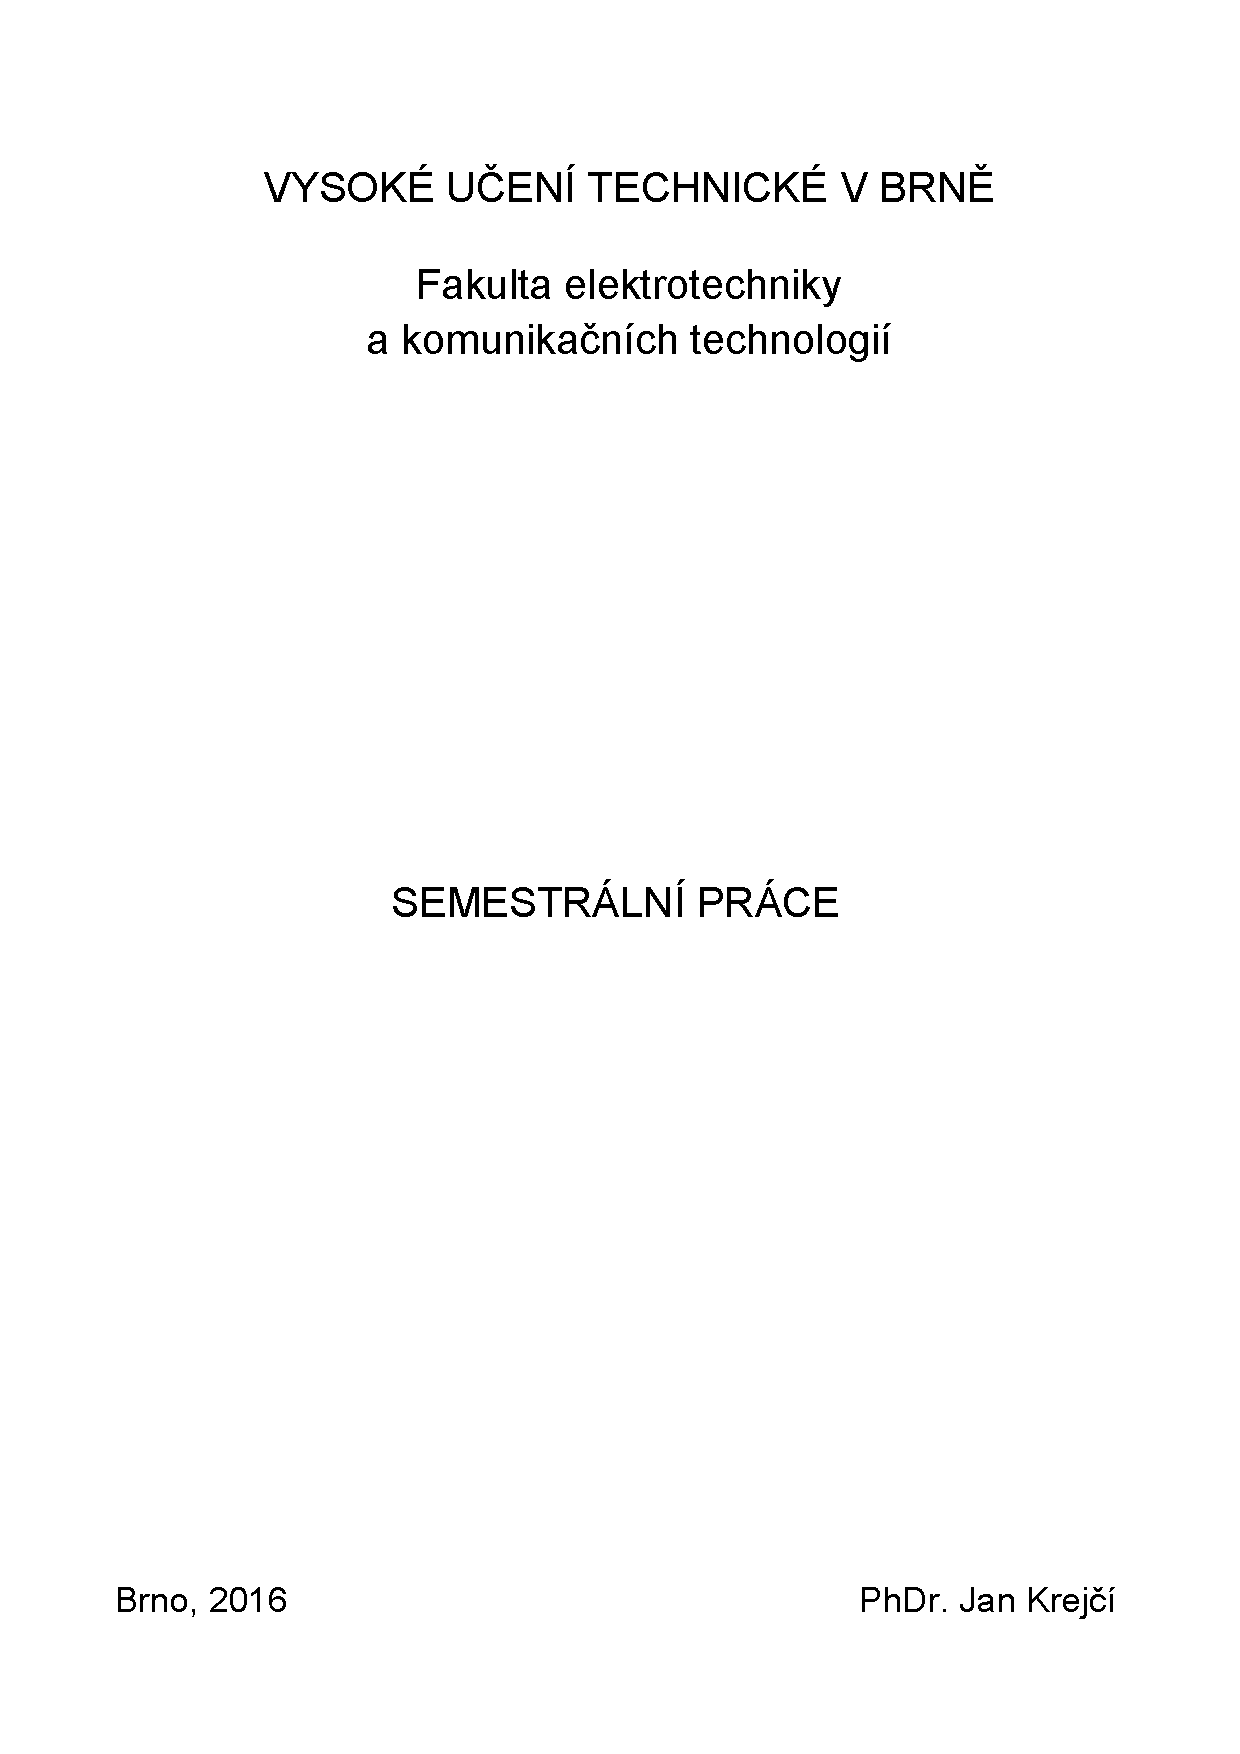
\includepdf[pages=1,offset=19mm 0mm]{pdf/student-desky}% název souboru nesmí obsahovat mezery!
% nebo vytvoření desek z balíčku
%\vytvorobalku
%\setcounter{page}{1} %resetovani citace stranek - desky se necisluji

%% Vložení titulního listu generovaného informačním systémem

\includepdf[pages=1,offset=19mm 0mm]{pdf/student-titulka}% název souboru nesmí obsahovat mezery!
% nebo vytvoření titulní stránky z balíčku
%\vytvortitulku
   
%% Vložení zadání generovaného informačním systémem
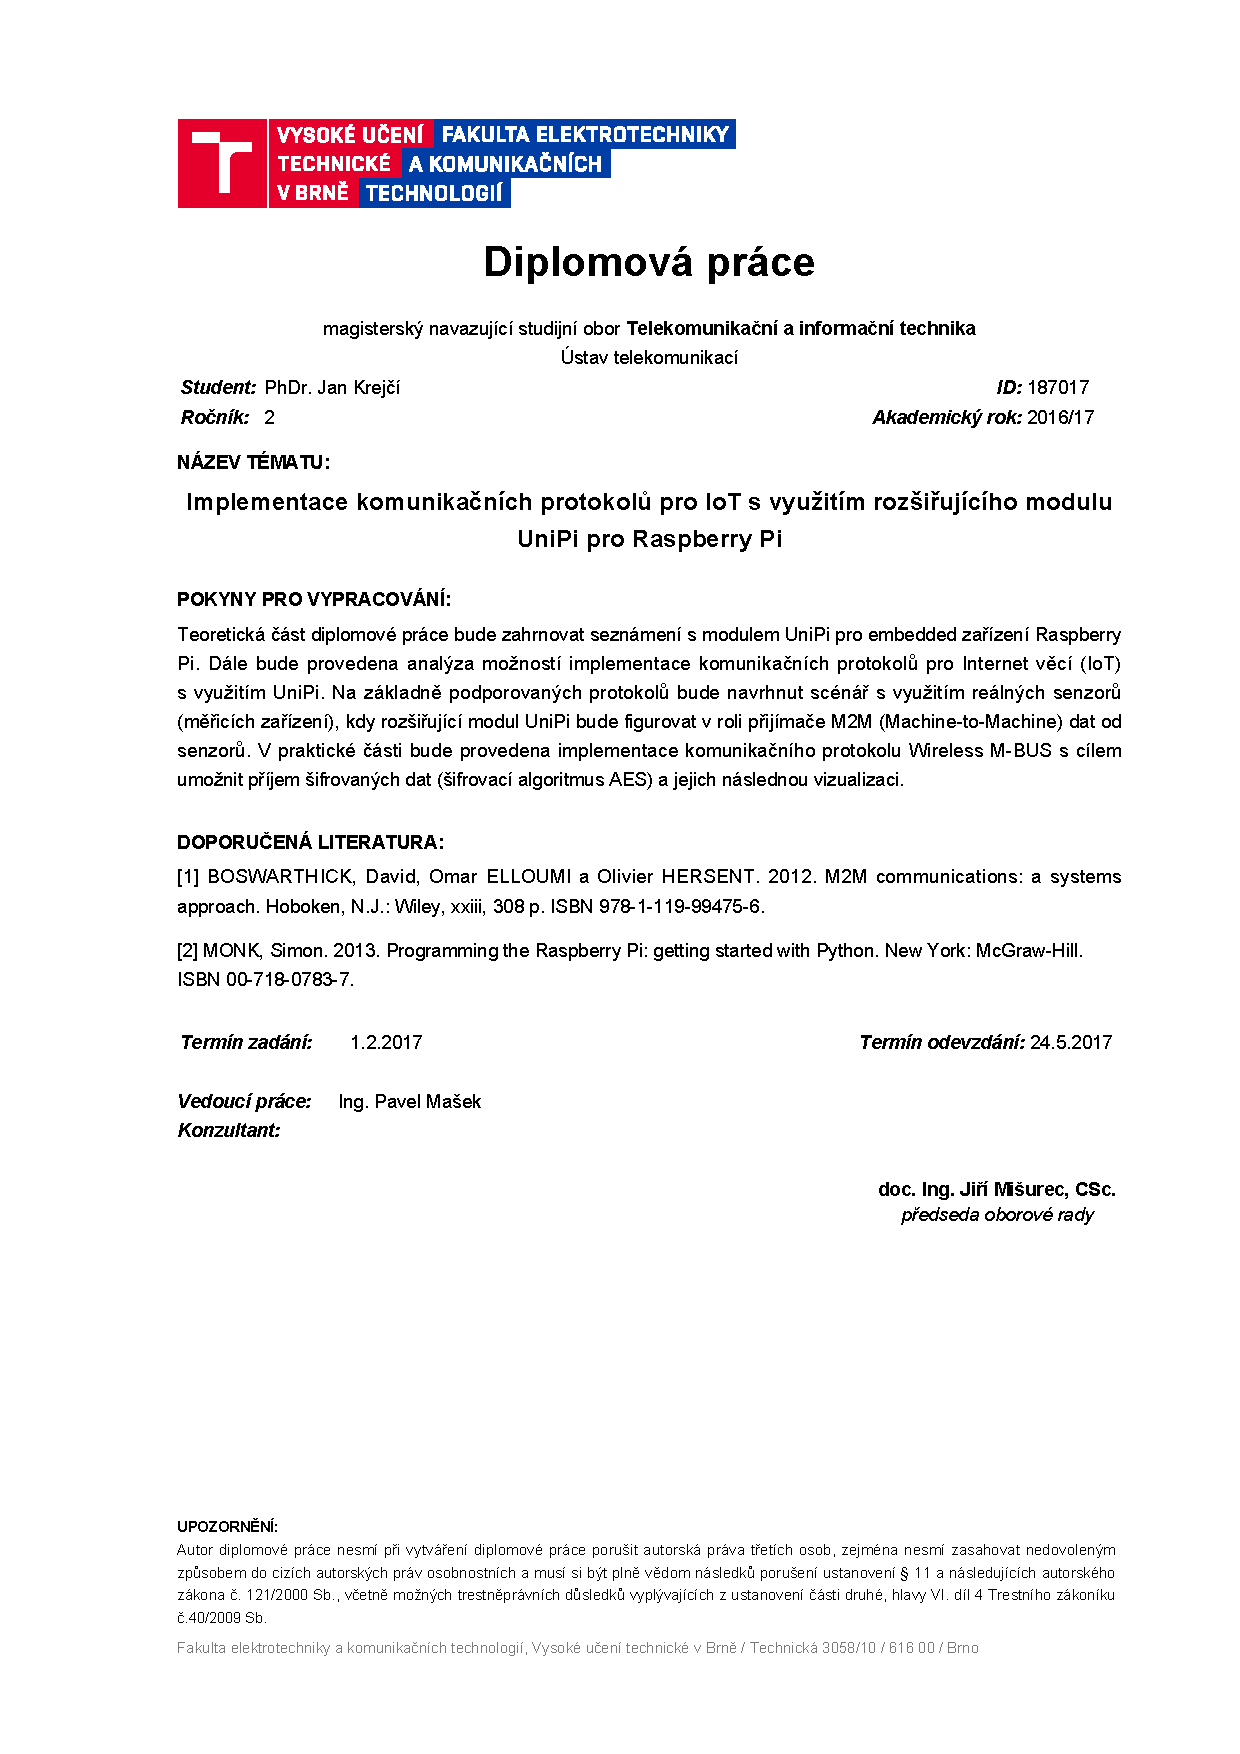
\includepdf[pages=1,offset=19mm 0mm]{pdf/student-zadani}% název souboru nesmí obsahovat mezery!
% nebo lze vytvořit prázdný list příkazem ze šablony
%\stranka{}%
%	{\sffamily\Huge\centering ZDE VLOŽIT LIST ZADÁNÍ}%
%	{\sffamily\centering Z~důvodu správného číslování stránek}

%% Vysázení stránky s abstraktem
\vytvorabstrakt

%% Vysázení prohlaseni o samostatnosti
\vytvorprohlaseni

%% Vysázení poděkování
\vytvorpodekovani

%% Vysázení poděkování projektu SIX
% ----------- zakomentujte pokud neodpovida realite
\vytvorpodekovaniSIX

%% Vysázení obsahu
\obsah

%% Vysázení seznamu obrázků
\seznamobrazku

%% Vysázení seznamu tabulek
\seznamtabulek

%% Vložení souboru 'text/uvod.tex'
\chapter*{Úvod}
\phantomsection
\addcontentsline{toc}{chapter}{Úvod}

Fenoménem dneška je propojování Internetu věcí (IoT - Internet of Things), služeb (IoS - Internet of Services) a lidí (IoP - Internet of People) a s ním související vývoj komunikací stroj-stroj (M2M - Machine to Machine), člověk-stroj (H2M - Human to Machine) nebo člověk-člověk (H2H - Human to Human). Internet věcí, služeb a lidí se rozšiřuje závratným tempem a proniká tak do odvětví, ve kterých se rostoucím tempem využívají tato zařízení a roste potřeba rozšíření těchto zařízení o nové komunikační protokoly a technologie. Vzniknou sítě založené na propojených zařízení, které budou schopny samostatné výměny informací, vyvolání potřebných akcí v reakci na momentální podmínky a vzájemné nezávislé kontroly. Senzory, přístroje a IT systémy budou vzájemně propojeny a budou na sebe pomocí standardních komunikačních protokolů vzájemně reagovat a analyzovat data, aby mohly předvídat případné chyby či poruchy, konfigurovat samy sebe a v reálném čase se přizpůsobovat změněným podmínkám \cite{Prumysl4PDF,Prumysl4Web}.

Tato práce vychází z požadavku na implementaci Wireless M-Bus protokolu do produktu UniPi NEURON. K tomuto účelu bylo zvoleno nízkovýkonové (embedded) zařízení RaspberryPi a jeho rozšiřující modul UniPi. Pro M2M (Machine to Machine) komunikaci byl zvolen protokol Wireless M-Bus, jelikož je jedním z nejrozšířenějších a navíc je založen na protokolu M-Bus, který je osvědčený a velmi rozšířený (měření a regulace topných systémů, plynu, odběru vody a elektrické energie). V teoretické části práce jsou popsány jednotlivé rodiny jednodeskových počítačů a jejich vlastnosti, popis rozšiřujících desek UniPi a samotného komunikačního modulu Wireless M-Bus a popis protokolu Wireless M-Bus. 

Praktická část se zaměřuje na implementaci Wireless M-Bus protokolu v zařízení RaspberryPi pomocí rozšiřujícího modulu UniPi a komunikačního modulu Wireless M-Bus. Tato implementace vyčítání dat ze vzdálených zařízení je nejprve realizována v jazyku Python a následně je tato komunikace implementována jako plugin do software Mervis.
 

%% Vložení kapitoly s kecama o IoT
\chapter{Internet věcí}

Cílem Internetu věcí (IoT - Internet of Things) je propojení zařízení, systémů a služeb za účelem poskytnutí více dat, která mohou být převedena na informace a informace potom na znalosti, které mohou být následně aplikovány. Princip IoT tedy je: na začátku je sběr dat, ty jsou následně uložena a analyzována a poté dojde ke sdílení výsledků. V rámci IoT se vytvořily dva hlavní směry, průmyslový internet věcí (iIoT - Industry IoT) a spotřebitelský internet věcí (cIoT - Customer IoT) \cite{iot_svet_hardware_internet_veci, iot_pohanka_internet_veci}. Rozdíly obou směrů jsou shrnuty v Tab.~\ref{TableIOT}.

\section{Spotřebitelský Internet věcí}
Spotřebitelský Internet věcí se zaměřuje na spotřebitelská zařízení, IT a telekomunikační zařízení a další. Jsou zde využívána zařízení zjednodušující každodenní život pomocí automatizace v domácnosti, chytrých zařízení nebo pomocí nositelné elektroniky. Hlavní výhodou je zvýšení uživatelského zážitku (QoE - Quality of Experience).

\section{Průmyslový Internet věcí}
Průmyslový Internet věci vychází z M2M (Machine to Machine) a rozšiřuje komuikaci o možnost uložení, analýzy a zobrazení dat. Jedná se o IoT zařízení a systémy, které jsou používány v průmyslových odvětvích, jako jsou průmyslová automatizace, energetický průmysl a zdravotnictví. Hlavním zaměřením je efektivnější využívání zdrojů, snížení provozních nákladů, zvýšení efektivity či bezpečnosti. V praxi může sloužit například pro zajištění bezpečnosti pracovníků či automatizaci údržby. 


\begin{table}[!ht]
\caption{Porovnání průmyslového a spotřebitelského IoT \cite{iot_svet_hardware_internet_veci, iot_pohanka_internet_veci}}
\label{TableIOT}
\begin{center}
\small
\begin{tabular}{|c|c|c|}
\hline
 & \textbf{Průmyslový IoT} & \textbf{Spotřebitelský IoT} \\ \hline
\textbf{Zaměření} & Průmysl & Spotřebitel \\ \hline
\textbf{Zařízení} & \begin{tabular}[c]{@{}c@{}}Stroje, zařízení\\  a průmyslová automatizace.\end{tabular} & \begin{tabular}[c]{@{}c@{}}Chytré zařízení\\ a nositelná elektronika.\end{tabular} \\ \hline
\textbf{Důležitost} & \begin{tabular}[c]{@{}c@{}}Jedná se o životně\\ důležité systémy.\end{tabular} & \begin{tabular}[c]{@{}c@{}}Nejedná se o životně \\ důležité systémy.\end{tabular} \\ \hline
\textbf{Využití} & \begin{tabular}[c]{@{}c@{}}Lepší využívání zdrojů, \\  snížení provozních nákladů, \\ zvýšení efektivity či bezpečnosti.\end{tabular} & \begin{tabular}[c]{@{}c@{}}Zvýšení uživatelského\\ zážitku.\end{tabular} \\ \hline
\end{tabular}
  \end{center}
\end{table}

\subsection{Průmysl 4.0}

Současný trend digitalizace a s ní související automatizace výroby je označován jako Průmysl 4.0. Koncept vychází z dokumentu, který byl představen na veletrhu v Hannoveru v roce 2013. Předpokládá se, že v horizontu následujících 10 až 15 let nastane příchod čtvrté průmyslové revoluce, která přinese radikální změnu ve srovnání s nynějším výrobním procesem. Podle této myšlenky vzniknou chytré továrny, které budou využívat kyberneticko-fyzikální systémy. Ty převezmou opakující se a jednoduché činnosti, které do té doby vykonávali lidé. Má zahrnovat kompletní digitalizaci, robotizaci a automatizaci většiny současných lidských činností pro zajištění větší rychlosti a efektivity výroby přesnějších, osobitějších, spolehlivějších a levnějších produktů, současně pro efektivnější využití materiálů a ekologičtějšímu průmyslu i lidskému životu.

	\begin{figure}[!ht]
  \begin{center}
   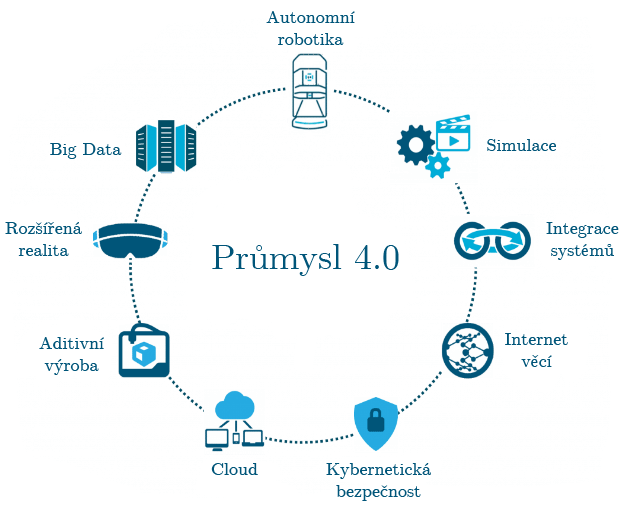
\includegraphics[scale=0.4]{obrazky/iot_industry4}
  \end{center}
  \caption{Schéma odvětví Průmyslu 4.0}
\end{figure}


Na průmyslové úrovni má jít o nahrazení manuální lidské práce robotizací, současné manuální zadávání výrobních dat a postupů má být nahrazeno automatickým elektronickým předáváním informací mezi jednotlivými výrobními komponentami a materiálmi. Významné změny mají i ve spojistosti s automatizovaným průmyslem nastat v oblasti domácností a běžného bydlení, kde mají být jednotlivé domácí systémy vzájemně elektronicky propojeny a jejich vzájemná koordinovaná spolupráce bude maximalizovat efektivitu a současně minimalizovat spotřebu médií.

V reflexi na tento trend vydalo v září 2015 vydalo Ministerstvo průmyslu a obchodu Národní iniciativu Průmysl 4.0~\cite{uvod_prumysl_4_pdf}, podle které bude revoluce příležitostí pro růst a konkurenceschopnost českých firem a České republiky vůbec.










%% Vložení kapitoly se srovnanim HW
\chapter{Embedded zařízení pro IoT}

V současnosti existuje velké množství zařízení v roli výpočetní jednotky, využitelných pro chytrou domácnost či Internet věcí. Tato kapitola představí nejznámější z nich, popíše jejich možnosti, uvede možnosti připojení senzorů a zmíní jejich nedostatky. 

Mezi nejznámější nízkovýkonové (embedded) zařízení patří open-source Arduino (Kap.~\ref{KapArduino}), RaspberryPi (Kap.~\ref{KapRaspi}) a jejich klony (Kap.~\ref{KapArduinoKlony} a \ref{KapRaspiKlony}). Poté budou zmíněny desky předních firem výrobců procesorů Intel (Kap.~\ref{KapIntel}) a AMD (Kap.~\ref{KapAMD}) a v neposlední řadě se podíváme na desky firmy CubieBoard (Kap.~\ref{KapCubie}), HardKernel (Kap.~\ref{KapKernel}) a další. 

Z výše uvedených byly vybrány jen nízkovýkonová zařízení, využitelná pro chytrou domácnost či Internet věcí, s vyvedenými GPIO piny a dostatečnou dokumentací.

Jejich vlastnosti jsou přehledně shrnuty v příloze \ref{PrilohaTabulkaTabulka}.

%%%%%%%%%%%%%%%%%%%%%%%%%%%%%%%%%%%%%%%%%%%%%%%%%%%%%%%%%%%%%%%%%%%%%%%%%%%%%%%%%%%%%%%%%%%%%%%%%%%%%%%%%%%%%%%%%
%%%%%%%%%%%%%%%%%%%%%%%%%%%%%%%%%%%%%%%%%%%%%%%%%%%%%%%%%%%%%%%%%%%%%%%%%%%%%%%%%%%%%%%%%%%%%%%%%%%%%%%%%%%%%%%%%
%%%%%%%%%%%%%%%%%%%%%%%%%%%%%%%%%%%%%%%%%%%%%%%%%%%%%%%%%%%%%%%%%%%%%%%%%%%%%%%%%%%%%%%%%%%%%%%%%%%%%%%%%%%%%%%%%
%%%%%%%%%%%%%%%%%%%%%%%%%%%%%%%%%%%%%%%%%%%%%%%%%%%%%%%%%%%%%%%%%%%%%%%%%%%%%%%%%%%%%%%%%%%%%%%%%%%%%%%%%%%%%%%%%
%%%%%%%%%%%%%%%%%%%%%%%%%%%%%%%%%%%%%%%%%%%%%%%%%%%%%%%%%%%%%%%%%%%%%%%%%%%%%%%%%%%%%%%%%%%%%%%%%%%%%%%%%%%%%%%%%
%%%%%%%%%%%%%%%%%%%%%%%%%%%%%%%%%%%%%%%%%%%%%%%%%%%%%%%%%%%%%%%%%%%%%%%%%%%%%%%%%%%%%%%%%%%%%%%%%%%%%%%%%%%%%%%%%

\section{Arduino}
\label{KapArduino}

Ardiuno je skupina několika jednodeskových počítačů založených mikrokontrolérech. Nejedná se však o klasický stolní počítač IBM PC, ale o protypovací desku, ke které se spíše jak ovládací  zobrazovací periferie připojují senzory, moduly, serva, displeje. Projekt je od svého počátku šířen jako open-source, příručka jazyka a externí knihovny jsou pak šířeny pod licencí Creative Commons.
	
Výrobce těchto desek vytvořil vývojové prostředí shodné pro všechny produkty Ardiuno. To se nazvývá Arduino IDE, je dostupné zdarma na webu výrobce a podporuje jazyk Wiring~\cite{embed_about_wiring_2011}, což je upravená verze jazyka C. Prostředí zároveň obsahuje i Serial Monitor, který slouží k oboustranné sériové komunikaci mezi Arduinem a PC. Alternativou ještě může být prostředí Processing~\cite{embed_about_processing_2015} využívající stejnojmenný jazyk, umožňující vytváření grafických multiplatformních aplikací.
	
Na deskách bývá několik diod, resetovací tlačítko, různé přídavné sběrnice (UART, I2C), konektory pro ICSP programování, napájecí konektor, oscilátor a obvod zprostředkovávající komunikaci po USB.
	
Arduino podporuje připojení rozšiřujících karet. Ty se u Arduina nazývají Shieldy, mají převážně stejný tvar jako deska Arduina a připojují se pomocí dlouhých pinů. Zabírají celou plochu, ale většina z nich dále zpřístupňuje GPIO (General Purpose Input/Output) piny, lze je tedy skládat na sebe. Stejně jako Arduino desek existuje i celá řada shieldů.
	
Samozřejmě lze k Arduinu připojit i samotné moduly nebo senzory, přímým připojením na dané piny. Je však třeba dbát na to, že Arduino pracuje s 5\,V logikou, zatímco například RaspberryPi pracuje s 3.3\,V logikou.
	
		\subsection{Arduino Duemilanove} Arduino Duemilanove je vývojová jednoprocesorová deska s mikroprocesorem ATMega168 od firmy Atmel, tedy platformě Atmel AVR. 
		Parametry: ATmega168 s 16\,MHz krystalem, 16\,KB flash, 1\,KB SRAM (Static Random Access Memory), 512\,B EEPROM (Electrically Erasable Programmable Read-Only Memory). 	Konektivita: 14 digitálních vstupně/výstupných pinů, z toho 6 z nich může být využito i PWM (Pulse Width Modulation) , vstupních analogových pinů (10\,bit A/D převodník, 0-5\,V), I2C (Inter-Integrated Circuit) sběrnici, UART (Universal Asynchronous Receiver/Transmitter) sběrnici, ICSP (In Circuit Serial Programming) rozhraní, USB (Universal Serial Bus) rozhraní~\cite{ArduinoDuemilanove}.	
	
		\subsection{Arduino Uno} Arduino Uno je v současné době asi nejčastěji používaný typ desky. Arduino Uno je vývojová jednoprocesorová deska s mikroprocesorem ATMega328. Od roku 2011 je nástupcem Arduina Duemilanove. Změny oproti předchůdci jsou pouze v použitém mikrokontroléru, došlo k zdvojnásobení velikosti paměti na 32\,KB flash, 2\,KB SRAM, 1\,KB EEPROM~\cite{ArduinoUno}.
	
		\subsection{Arduino Leonardo} 
		Arduino Leonardo designově navazuje na Arduino Uno, liší se pouze v použitém čipu ATmega32u4~\cite{ArduinoLeonardo}.


\begin{figure*}[!ht]
    \centering
			\subfigure[Arduino Duemilanove]{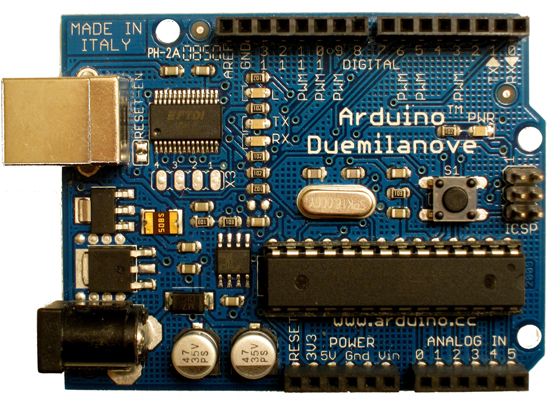
\includegraphics[width=0.3\textwidth]{obrazky/emded_arduino_duemilanove}\label{emded_arduino_duemilanove}}
			\hspace*{5mm}
			\subfigure[Arduino Uno]{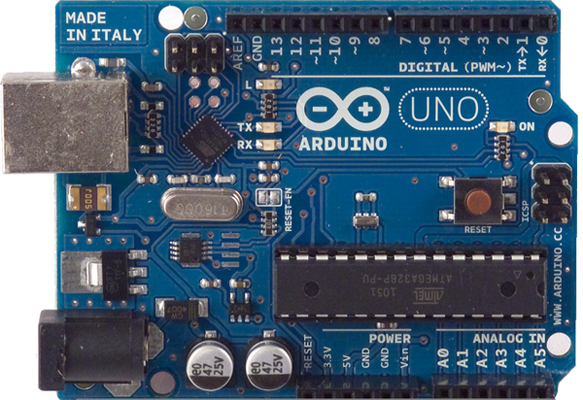
\includegraphics[width=0.3\textwidth]{obrazky/emded_arduino_uno}\label{emded_arduino_uno}}
			\hspace*{5mm}
			\subfigure[Arduino Leonardo]{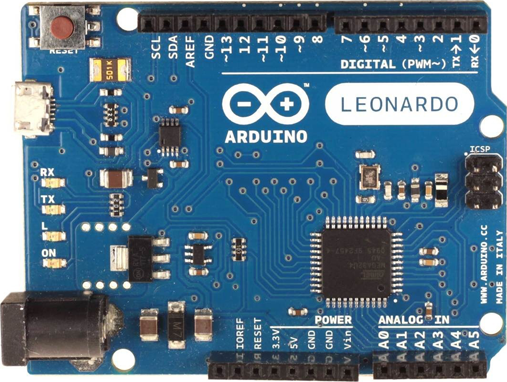
\includegraphics[width=0.3\textwidth]{obrazky/emded_arduino_leonardo}\label{emded_arduino_leonardo}}
    \caption{Arduino Duemilanove, Uno a Leonardo}
\end{figure*}


\newpage
	
					\subsection{Arduino Mega} 
					Arduino Mega je deska pro náročnější projekty. Oproti klasickému Arduinu má Arduino Mega rychlejší procesor (16\,MHz) a také více vstupních a výstupních pinů. K dispozici je 54 digitálních pinů, 14 PWM výstupů, 16 analogových vstupů a 4 hardwarové sériové porty. Dále má 256\,kB flash paměti, 8\,kB RAM paměti a 4\,kB EEPROM paměti~\cite{ArduinoMega}.	
			
		\subsection{Arduino Due} 
		Arduino Due je nástupcem Arduino Mega a je to první karta Arduino, na níž je umístěn 32-bitový řadič (32-bitový ARM procesor
		Atmel SAM3X8E). Vysoká taktovací rychlost 84\,MHz ve spojení s celkem 54 I/O piny umožňuje realizaci značně rozsáhlých projektů. K 54 pinům mimo jiné patří 12 PWM výstupů a 12 analogových vstupů, 4 UARTy, 2 I2C a dvojitý digitálně-analogový měnič. Vlastní USB Host poskytuje kartě vedle standardů jako JTAG (Joint Test Action Group), SPI (Serial Peripheral Interface) a Micro USB širší možnosti konektivity~\cite{ArduinoDue}.	

\begin{figure*}[!ht]
    \centering
			\subfigure[Arduino Mega]{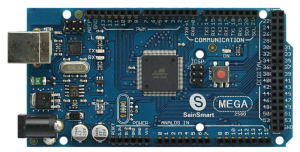
\includegraphics[width=0.45\textwidth]{obrazky/emded_arduino_mega}\label{emded_arduino_mega}}
			\hspace*{5mm}
			\subfigure[Arduino Due]{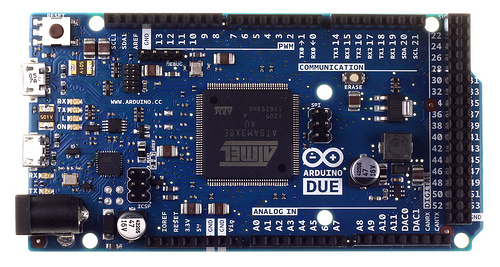
\includegraphics[width=0.45\textwidth]{obrazky/emded_arduino_due}\label{emded_arduino_due}}
		\caption{Arduino Mega a Due}
\end{figure*}


	\subsection{Arduino Mini} 
	Arduino Mini je asi nejmenší oficiální verze Arduina, navržená pro úsporu místa. Daní za malé rozměry je však absence USB portu. K programování je tedy nutné použít externí USB2Serial převodník. Jeho výkon však nijak nezaostává za většími deskami. Běží na procesoru ATmega328 s taktem 16\,MHz. Pro své malé rozměry je vhodný k použití například v chytrých vypínačích, či dálkových ovladačích~\cite{ArduinoMini}.	
	
	\subsection{Arduino Micro} 
	Arduino Micro je jedna z desek, která má čip obsahující předprogramovaný převodník ATmega32u4~\cite{ArduinoMicro}.	 
		
	\subsection{Arduino Nano} 
	Arduino Nano navíc obsahuje ještě USB port a převodník~\cite{ArduinoNano}.	
		
\begin{figure*}[!ht]
    \centering
			\subfigure[Arduino Mini]{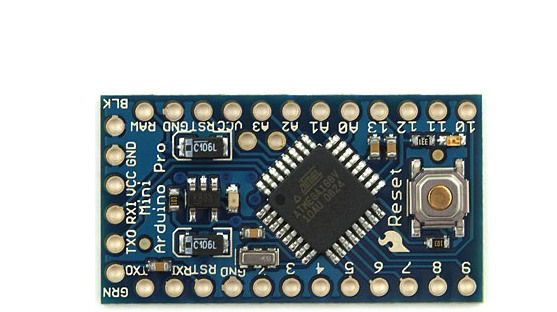
\includegraphics[width=0.3\textwidth]{obrazky/emded_arduino_mini}\label{emded_arduino_mini}}
			\hspace*{5mm}
			\subfigure[Arduino Micro]{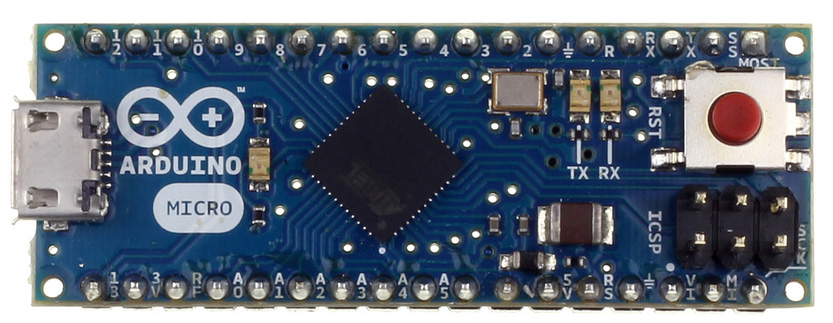
\includegraphics[width=0.3\textwidth]{obrazky/emded_arduino_micro}\label{emded_arduino_micro}}
			\hspace*{5mm}
			\subfigure[Arduino Nano]{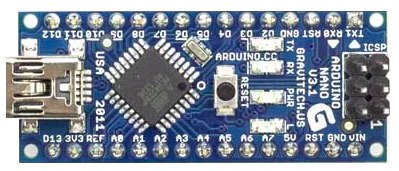
\includegraphics[width=0.3\textwidth]{obrazky/emded_arduino_nano}\label{emded_arduino_nano}}
		\caption{Arduino Mini, Micro a Nano}
\end{figure*}
	
		
		\subsection{Arduino Fio} 
		Arduino Fio je přizpůsobená k připojení různých bezdrátových modulů (například ZigBee nebo XBee moduly). Základem je procesor ATmega328P, který běží na frekvenci 8\,MHz. Napětí je zde kvůli kompatibilitě s moduly sníženo oproti většině ostatních desek z 5\,V na 3,3\,V~\cite{ArduinoFio}.	
		
	\subsection{Arduino MKR1000}
	Arduino MKR1000 je postavené na čipu ATSAMW25 od Atmelu, který v sobě spojuje ARMové jádro SAMD21 Cortex-M, Wi-Fi čip a šifrovací a autentizační čip ECC508. Tento čip nabízí ECDH (Diffie-Hellman s využitím eliptických křivek) a ECDSA (Elliptic Curve Digital Signature Algorithm). Dále pak generátor náhodných čísel, unikátní 72bitové sériové číslo nebo SHA-256 s volitelným HMAC.
	
	
	\begin{figure*}[!ht]
    \centering
			\subfigure[Arduino Fio]{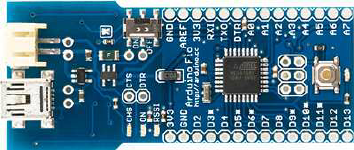
\includegraphics[width=0.33\textwidth]{obrazky/emded_arduino_fio}\label{emded_arduino_fio}}
			\hspace*{5mm}
			\subfigure[Arduino MKR1000]{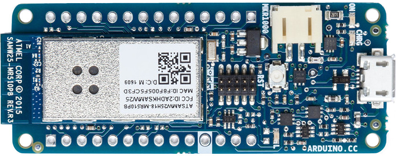
\includegraphics[width=0.33\textwidth]{obrazky/emded_arduino_mkr1000}\label{emded_arduino_mkr1000}}
		\caption{Arduino Fio a MKR1000}
\end{figure*}
	
		\subsection{Lilypad Arduino} 
		Lilypad Arduino je postaveno na ATmega168V (energeticky úsporná verze ATmega168) nebo ATmega328V. Je určena wearables projekty, zejména pro implementaci do textilií, kdy jsou spoje tvořeny vodivou nití. Není však pratelná. Existuje více variant této desky~\cite{ArduinoLilipad}.	
	
	\begin{figure*}[!ht]
    \centering
			\subfigure[Lilypad Arduino ]{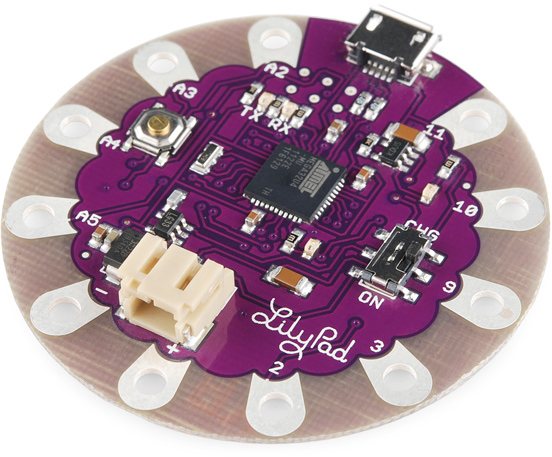
\includegraphics[width=0.55\textwidth]{obrazky/emded_arduino_lilipad}\label{emded_arduino_lilipad}}
			\hspace*{5mm}
			\subfigure[Arduino Yun ]{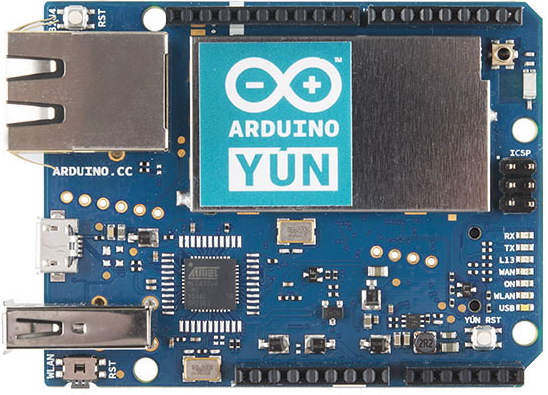
\includegraphics[width=0.35\textwidth]{obrazky/emded_arduino_yun}\label{emded_arduino_yun}}
					\caption{Lilypad Arduino a Arduino Fio}
\end{figure*}
	
	
	\subsection{Arduino Yun} 
	Arduino Yun je deska založená na ATmega32u4 a Atheros AR9331, který je schopný běhu odlehčeného linuxu Linino. Ve výbavě je softwarový bridge (prostředník, most), který zajišťuje komunikaci mezi oběma čipy. Procesor Atheros podporuje linuxové distribuce založené na OpenWrt s názvem OpenWrt-Yun. Deska má vestavěný Ethernet a WiFi modul, USB-A port, slot pro MicroSD kartu. Dále disponuje 20 digitálními I/O piny, z toho 7 mohou být použito jako výstupy PWM a 12 jako analogové vstupy~\cite{ArduinoYun}.	


	
%%%%%%%%%%%%%%%%%%%%%%%%%%%%%%%%%%%%%%%%%%%%%%%%%%%%%%%%%%%%%%%%%%%%%%%%%%%%%%%%%%%%%%%%%%%%%%%%%%%%%%%%%%%%%%%%%
%%%%%%%%%%%%%%%%%%%%%%%%%%%%%%%%%%%%%%%%%%%%%%%%%%%%%%%%%%%%%%%%%%%%%%%%%%%%%%%%%%%%%%%%%%%%%%%%%%%%%%%%%%%%%%%%%
%%%%%%%%%%%%%%%%%%%%%%%%%%%%%%%%%%%%%%%%%%%%%%%%%%%%%%%%%%%%%%%%%%%%%%%%%%%%%%%%%%%%%%%%%%%%%%%%%%%%%%%%%%%%%%%%%
%%%%%%%%%%%%%%%%%%%%%%%%%%%%%%%%%%%%%%%%%%%%%%%%%%%%%%%%%%%%%%%%%%%%%%%%%%%%%%%%%%%%%%%%%%%%%%%%%%%%%%%%%%%%%%%%%
%%%%%%%%%%%%%%%%%%%%%%%%%%%%%%%%%%%%%%%%%%%%%%%%%%%%%%%%%%%%%%%%%%%%%%%%%%%%%%%%%%%%%%%%%%%%%%%%%%%%%%%%%%%%%%%%%
%%%%%%%%%%%%%%%%%%%%%%%%%%%%%%%%%%%%%%%%%%%%%%%%%%%%%%%%%%%%%%%%%%%%%%%%%%%%%%%%%%%%%%%%%%%%%%%%%%%%%%%%%%%%%%%%%

\section{Arduino klony}
\label{KapArduinoKlony}

	Jelikož je projekt Arduino open-source, vzniklo množství klonů od dalších firem i jednotlivců. Klony jsou s původním Arduinem kompatibilní, ve většině případů konfigurací odpovídají některému z Arduino modelu, většinou Arduino UNO. Kity, které nemají shodné rozložení pinů neumožňují připojení Arduino shieldů. V této podkapitole je uveden krátký přehled těch nejznámějších. Rozsáhlý přehled kompatibilních klonů lze nalézt na oficiálních stránkách Arduina~\cite{ArduinoClonesWeb}.
	
	\subsection{Freeduino} 
	Freeduino je klon Arduina, vycházející z Arduino Diecimila.
	
	\subsection{LABduino} 
	LABduino je český klon Arduina vytvořený z otevřené elektronické stavebnice MLAB.
	
	\subsection{Arduelo Libero}	
	Arduelo Libero je mírně vylepšený český free klon Arduino Diecimila.
	
	\subsection{Bare Bones Board} 
	Bare Bones Board je kompatibilní deska, tvarově nepřipomínající žádný Arduino produkt. Kvůli rozložení pinů nepodporující shieldy. Vyráběná a prodávané jako kit firmou Modern Device Company.
	
	\begin{figure*}[!ht]
    \centering
			\subfigure[Bare Bones Board]{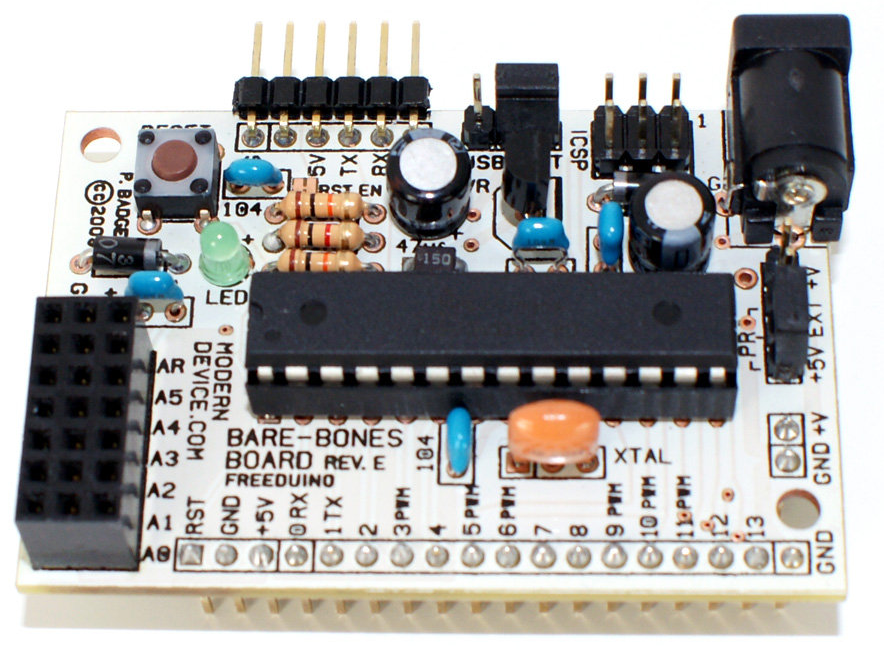
\includegraphics[width=0.45\textwidth]{obrazky/embed_barebones}\label{emded_barebones}}
			\hspace*{5mm}
			\subfigure[Freaduino]{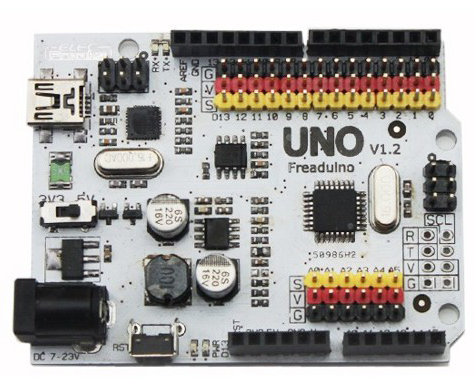
\includegraphics[width=0.45\textwidth]{obrazky/embed_freaduino}\label{emded_freaduino}}
					\caption{Bare Bones Board a Freaduino}
	\end{figure*}	
		
	\subsection{Freaduino} 
	Freaduino je kompatibilní deska, tvarově shodná s Arduino UNO, vyráběná a prodávaná firmou ElecFreak jako kit The Freaduino Uno. Podporuje 3.3\,V logiku a napájení. Má piny na připojení modulů (XBee). Napájecí piny zvládají zátěž až 2\,A.
	
	\subsection{Runtime} 
	Runtime je kompatibilní deska, tvarově nepřipomínající žádný Arduino produkt. Kvůli rozložení pinů nepodporující shieldy. Vyráběná a prodávaná jako kit firmou NKC Electronics.
	
	\subsection{Nanode} 
	Nanode je kompatibilní deska, tvarově nepřipomínající žádný Arduino produkt. Tvarově připomíná Arduino UNO, rozložení pinů je kompatibilní.
	
	\subsection{Seeeduino} 
	Seeeduino je kompatibilní deska, vzhledem připomínající Arduino UNO, parametricky shodná s Arduino Mega.
	
	\subsection{Teensy}
	Teensy je kompletní vývojový mikrokontrolérový systém na velmi malé desce bez osazených pinů, který je schopen realizovat mnoho typů projektů. Softwarově je kompatibilní s Arduinem, programuje se však pomocí doplňku do Arduino IDE nebo pomocí WinAVR~\cite{ArduinoTeensy}.
	
	\subsection{Diavolino} 
	Diavolino je free klon Arduina, vzhledově i parametricky podobný Arduino UNO, bez vyvedených konektorů. Vyráběná a prodávané jako kit firmou Evil Mad Scientist.
		
\begin{figure*}[!ht]
    \centering
			\subfigure[Diavolino]{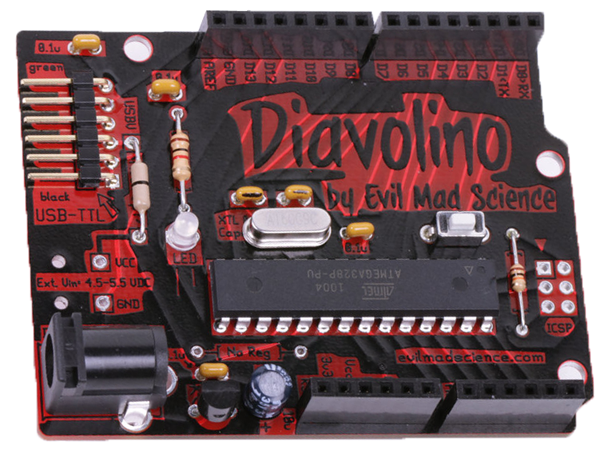
\includegraphics[width=0.45\textwidth]{obrazky/embed_diavolino}\label{emded_diavolino}}
			\hspace*{5mm}
			\subfigure[Boarduino]{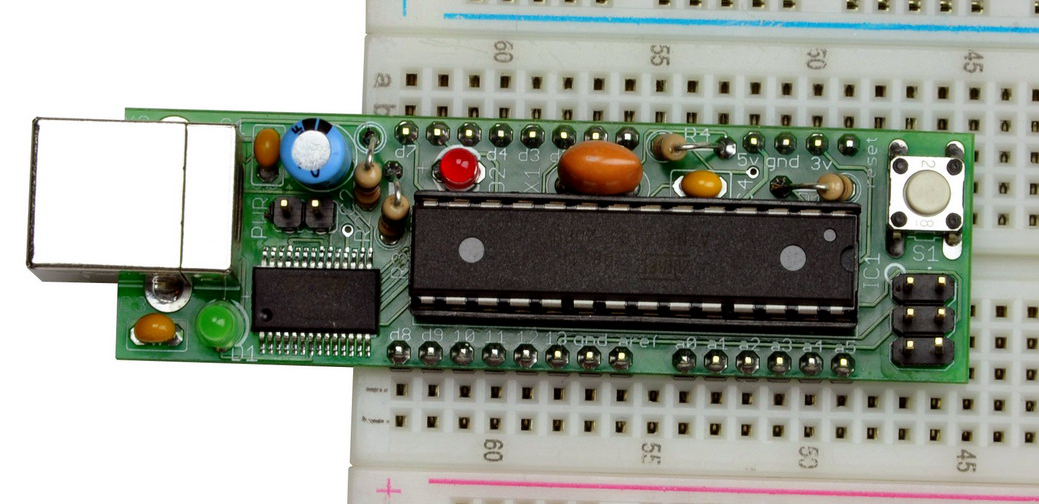
\includegraphics[width=0.45\textwidth]{obrazky/embed_boarduino}\label{emded_boarduino}}
					\caption{Diavolino a Boarduino}
	\end{figure*}		
	
	\subsection{Boarduino} 
	Boarduino je levnější klon Arduina Diecimila s piny pro zapojení rovnou do nepájivého pole.


%%%%%%%%%%%%%%%%%%%%%%%%%%%%%%%%%%%%%%%%%%%%%%%%%%%%%%%%%%%%%%%%%%%%%%%%%%%%%%%%%%%%%%%%%%%%%%%%%%%%%%%%%%%%%%%%%
%%%%%%%%%%%%%%%%%%%%%%%%%%%%%%%%%%%%%%%%%%%%%%%%%%%%%%%%%%%%%%%%%%%%%%%%%%%%%%%%%%%%%%%%%%%%%%%%%%%%%%%%%%%%%%%%%
%%%%%%%%%%%%%%%%%%%%%%%%%%%%%%%%%%%%%%%%%%%%%%%%%%%%%%%%%%%%%%%%%%%%%%%%%%%%%%%%%%%%%%%%%%%%%%%%%%%%%%%%%%%%%%%%%
%%%%%%%%%%%%%%%%%%%%%%%%%%%%%%%%%%%%%%%%%%%%%%%%%%%%%%%%%%%%%%%%%%%%%%%%%%%%%%%%%%%%%%%%%%%%%%%%%%%%%%%%%%%%%%%%%
%%%%%%%%%%%%%%%%%%%%%%%%%%%%%%%%%%%%%%%%%%%%%%%%%%%%%%%%%%%%%%%%%%%%%%%%%%%%%%%%%%%%%%%%%%%%%%%%%%%%%%%%%%%%%%%%%
%%%%%%%%%%%%%%%%%%%%%%%%%%%%%%%%%%%%%%%%%%%%%%%%%%%%%%%%%%%%%%%%%%%%%%%%%%%%%%%%%%%%%%%%%%%%%%%%%%%%%%%%%%%%%%%%%

\section{RaspberryPi}
\label{KapRaspi}

RaspberryPi reprezentuje jednodeskový počítač o velikosti zhruba platební karty. Byl vyvinut v roce 2012 s cílem podpořit výuku informatiky a seznámit studenty s řízením různých zařízení přes počítač~\cite{Raspi}. 

Primárním operačním systémem je Linux, k dispozici je několik jeho distribucí, případně lze použít Windows 10 IoT Core. Na rozdíl do Arduina obsahuje RaspberryPi plnohodnotný operační systém, ARM mikrokontrolér, USB pro připojení myši a klávesnice, ethernet konektor pro připojení sítě, grafický výstup HDMI (High-Definition Multimedia Interface) a kompozitní video, DSI (Display Serial Interface) pro připojení displeje, CSI (Camera Serial Interface) pro připojení kamery a čtečku pamětových karet, tedy působí spíše jako menší počítač, než vývojová platforma. 

Všechny další rozšiřující sběrnice (UART, I2C, SPI, PWM, digitální vstup a výstup, analogový vstup) jsou vyvedeny do 26-40 pinového GPIO konektoru. Na rozdíl od Arduina je možné RaspberryPi pomocí GPIO kontaktů použít nejen k ovládání různých zařízení, ale i k samotnému vývoji příslušných aplikací. Lze ho také použít jako multimediální přehrávač videa nebo hudby nebo i jen pro přístup k Internetu.

RaspberryPi stejně jako Arduino podporuje připojení rozšiřujících karet:

\begin{itemize}
	\item \textbf{Pi T-Cobbler} je pasivní elektronický přípravek, který se k RaspberryPi připojuje pomocí 40 žilového plochého kabelu a slouží k vyvedení pinů do vývojové desky breadboard. Zde na konektorové desce jsou již jednotlivé piny popsány.
\item \textbf{Gertboard}~\cite{GertBoard} je rozšiřující deska autora Gerta Van Loo, který rozšiřuje I/O možnosti RaspberryPi. K ní se připojuje pomocí 40 žilového plochého kabelu a rozšiřuje možnosti o 8/10/12-bitový dvoukanálový D/A převodník, 10-bitový dvoukanálový A/D převodník, obvody pro řízení motoru, předprogramovaný Atmel AVR ATmega 328P, 6 výstupů s otevřeným kolektorem a dalších 12 IO pinů. 
\item \textbf{UniPi} je rozšiřující deska která rozšiřuje I/O možnosti RaspberryPi. K ní se připojuje pomocí 26 žilového plochého kabelu a dle typu připojeného UniPi zařízení poskytuje I/O funkce navíc. Rozšiřujícími moduly UniPi se bude blíže zabývat následující kapitola (Kap.~\ref{KapUnipi}).
\item \textbf{RaspberryPi to Arduino Shield} je rozšiřující deska, která umožňuje propojení RasbperryPi a vybraných modelu Arduino.
\end{itemize}
Samozřejmě lze k Arduinu připojit i samotné moduly nebo senzory, přímým připojením na dané piny GPIO konektoru. Je však třeba dbát na to, že RaspberryPi pracuje s 3.3\,V logikou, zatímco například Arduino pracuje s 5\,V logikou. Popis GPIO konektoru včetně možností připojení je součástí následující kapitoly (Kap.~\ref{KapGPIO}).

	\subsection{RaspberryPi}
	Původní model RaspberryPi~\cite{RaspiOne} byl zveřejněn v únoru roku 2012. Obsahuje jednojádrový procesor na frekvenci 700\,MHz. U této verze existovaly tři modely:
	
		\begin{itemize}
		\item \textbf{Model A+} je odlehčená levná verze modelu B. Nemá žádný pamětový slot. Disponuje 256\,MB RAM. Neobsahuje USB port. Má 40 GPIO pinů.
		\item \textbf{Model B} byl původní RaspberryPi. Má slot na SD kartu. Disponuje 512\,MB RAM. Obsahuje 1 USB port. Má 26 GPIO pinů. Má samostatný výstup kompozitního videa.
		\item \textbf{Model B+} obsahuje   Má slot na MicroSD kartu. Disponuje 512\,MB RAM. Obsahuje 2 USB porty. Má 40 GPIO pinů.
	\end{itemize}
	
\begin{figure*}[!ht]
    \centering
			\subfigure[Model A+]{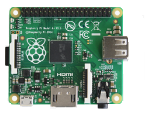
\includegraphics[width=0.3\textwidth]{obrazky/embed_raspi_1a}\label{embed_raspi_1a}}
			\hspace*{5mm}
			\subfigure[Model B]{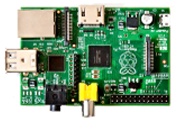
\includegraphics[width=0.3\textwidth]{obrazky/embed_raspi_1b}\label{embed_raspi_1b}}
			\hspace*{5mm}
			\subfigure[Model B+]{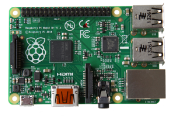
\includegraphics[width=0.3\textwidth]{obrazky/embed_raspi_1bp}\label{embed_raspi_1bp}}
		\caption{RaspberryPi prvních verzí}
\end{figure*}
	
	\subsection{RaspberryPi 2}
	RaspberryPi 2 je pokračováním RaspBerryPi, které přináší zejména vyšší výkon. Díky čtyřjádrovému procesoru BCM2836 o taktu 900 MHz by měl být 3–6× rychlejší než jeho předchůdce. Tento model disponuje 1 GB paměti a má 4 USB porty~\cite{RaspiTwo}.


\subsection{RaspberryPi 3}
		RaspberryPi 3, dostupný od roku 2016 je vybaven čtyřjádrovým 64bitovým procesorem ARM Cortex-A53 o taktu 1,2 GHz. Oproti předchozímu modelu přináší integraci WiFi a Bluetooth modulů přímo na desce a měl by být 2x rychlejší~\cite{RaspiThree}.
		

	
\subsection{RaspberryPi Zero}
		RaspberryPi Zero je nejúspornější varianta RaspberryPi, ideální pro použití v IoT. Vychází z modelu A+, ve srovnání s ním nabízí procesor s frekvencí 1 GHz a 512 MB paměti. Má přibližně poloviční velikost, nemá však vyvedené piny GPIO konektoru, USB konektory má ve verzi micro a HDMI ve verzi mini~\cite{RaspiZero}.

\begin{figure*}[!ht]
    \centering
			\subfigure[RaspberryPi 2]{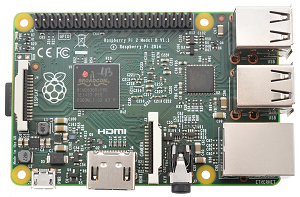
\includegraphics[width=0.3\textwidth]{obrazky/embed_raspi_2}\label{embed_raspi_2}}
			\hspace*{5mm}
			\subfigure[RaspberryPi 3]{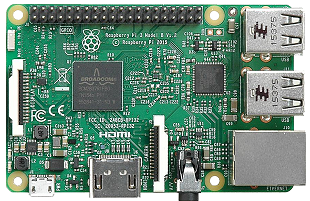
\includegraphics[width=0.3\textwidth]{obrazky/embed_raspi_3}\label{embed_raspi_3}}
			\hspace*{5mm}
			\subfigure[RaspberryPi Zero]{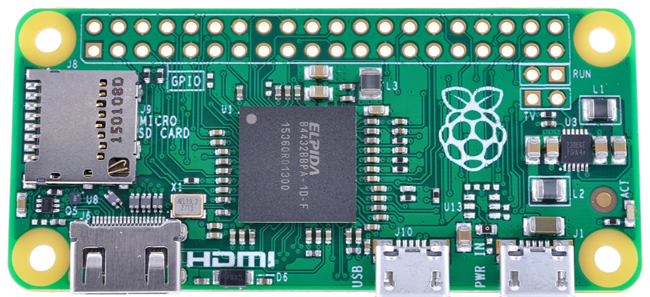
\includegraphics[width=0.3\textwidth]{obrazky/embed_raspi_zero}\label{embed_raspi_zero}}
		\caption{RaspberryPi následujících verzí}
\end{figure*}


%%%%%%%%%%%%%%%%%%%%%%%%%%%%%%%%%%%%%%%%%%%%%%%%%%%%%%%%%%%%%%%%%%%%%%%%%%%%%%%%%%%%%%%%%%%%%%%%%%%%%%%%%%%%%%%%%
%%%%%%%%%%%%%%%%%%%%%%%%%%%%%%%%%%%%%%%%%%%%%%%%%%%%%%%%%%%%%%%%%%%%%%%%%%%%%%%%%%%%%%%%%%%%%%%%%%%%%%%%%%%%%%%%%
%%%%%%%%%%%%%%%%%%%%%%%%%%%%%%%%%%%%%%%%%%%%%%%%%%%%%%%%%%%%%%%%%%%%%%%%%%%%%%%%%%%%%%%%%%%%%%%%%%%%%%%%%%%%%%%%%
%%%%%%%%%%%%%%%%%%%%%%%%%%%%%%%%%%%%%%%%%%%%%%%%%%%%%%%%%%%%%%%%%%%%%%%%%%%%%%%%%%%%%%%%%%%%%%%%%%%%%%%%%%%%%%%%%
%%%%%%%%%%%%%%%%%%%%%%%%%%%%%%%%%%%%%%%%%%%%%%%%%%%%%%%%%%%%%%%%%%%%%%%%%%%%%%%%%%%%%%%%%%%%%%%%%%%%%%%%%%%%%%%%%
%%%%%%%%%%%%%%%%%%%%%%%%%%%%%%%%%%%%%%%%%%%%%%%%%%%%%%%%%%%%%%%%%%%%%%%%%%%%%%%%%%%%%%%%%%%%%%%%%%%%%%%%%%%%%%%%%

\section{RaspberryPi klony}
\label{KapRaspiKlony}

Vzrůstající popularita RaspberryPi dala stejně jak u Arduina vzniknout celé řadě klonů. Tyto klony odvozují ze základního sestavení Raspberry Pi a určitým způsobem ho rozřišují. Jelikož označení „Raspberry Pi“ je registrovanou ochrannou známkou, proto mají podobně navžené počítače odvozené názvy, jako Banana Pi a Orange Pi. Zmíněné kony patří k nejznámějším a každý z nich již existuje v několika verzích, v této podkapitole budou představeny ty nejznámější s uvedením jejich hlavních odchylek od Raspberry Pi.

%%% ======================================= BANANA PI ============================== %%%
	\subsection{BananaPi}
		Původní Banana Pi, ze kterého vychází řada dalších modelů, je malý jednodeskový počítač, který se na první pohled podobá RaspberryPi.  Obsahuje dvoujádrový procesor a 512\,MB RAM. Na rozdíl od Raspberry Pi obsahuje Banana Pi také SATA řadič, mikrofon, který je připájen přímo na desce, gigabitový ethernet, USB 2.0 OTG, IR přijímač, tlačítko reset a power. Počítač podporuje SATA disky až do velikosti 2\,TB. GPIO konektor je vždy kompatibilni s některou verzi RaspberryPi. Za výrobou všech počítačů Banana Pi stojí čínská firma SinoVoip CO., Limited~\cite{BananaPi}.
		
	\textbf{BananaPi BPI-M2} je klon RaspberryPi 2, obsahuje taktéž čtyřjádrový procesor běžící na 1 GHz, má již integrovanou WiFi (Wireless Fidelity), ale neobsahuje SATA (Serial Advanced Technology Attachment) port.
	
	\textbf{BananaPi BPI-M3} obsahuje osmijádrový procesor 1,8\,GHz s 2\,GB RAM, dále zahrnuje Wifi b/g/n a integrované Bluetooth 4. Obsahuje SATA port.
	
	\textbf{BananaPi BPI-M64} obsahuje čtyřjádrový 64 bitový SoC procesor Allwinner A64.
	
	
	\begin{figure*}[!ht]
    \centering
			\subfigure[BananaPi BPI-M2]{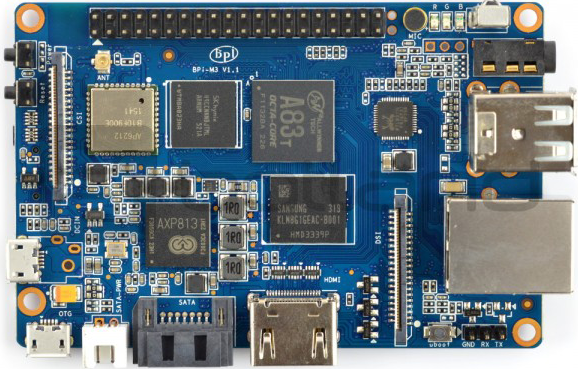
\includegraphics[width=0.45\textwidth]{obrazky/embed_bananapim2}\label{embed_bananapim2}}
			\hspace*{5mm}
			\subfigure[OrangePi Plus2]{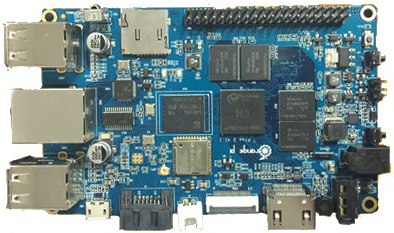
\includegraphics[width=0.45\textwidth]{obrazky/embed_orangepiplus2}\label{embed_orangepiplus2}}
			\caption{BananaPi BPI-M2 a OrangePi Plus2}
\end{figure*}
	
	

	%%% ======================================= ORANGE PI ============================== %%%
	\subsection{OrangePi}
	OrangePi je alternativa pro RaspberryPi vznikající v posledních dvou letech. Všechny modely jsou založeny na architektuře ARM Cortex-A7 s SoC Allwinner H3 s čtyřjádrovým CPU, výjimkou jsou OrangePi a OrangePi Mini, které mají SoC Allwinner A20 s dvojádrovým CPU. Grafickým čipem je u všech modelů ARM Mali-400 MP2. Všechny modely podporují HDMI CEC~\cite{OrangePi}.

		\textbf{OrangePi} je základní model z rodiny OrangePi, obsahuje čtyřjádrový procesor Allwinner A20 na 1\,GHz a 1\,GB RAM. Oproti RaspberryPi má navíc pouze mikrofon, IR (Infrared Radiation) port, USB OTG, ale nemá DSI rozhraní.
		
		\textbf{OrangePi Plus } má procesory běžící na 1,6\,GHz, 1\,GB RAM a 8\,GB EMMC Flash Oproti  RaspberryPi má gigabitový ethernet, integrovaný mikrofon, USB-OTG konektor, integrovaný WiFi modul, IR přijímač. Obsahuje SATA port, který je připojený přes USB převodník.
		
		\textbf{OrangePi Plus2} oproti předchozí verzi došlo k navýšení pamětí na 2\,GB RAM a 16\,GB EMMC Flash a doplnění CSI konektoru.
		
		\textbf{OrangePi One} vznikla jako reakce na odlehčenou verzi RaspberryPi Zero. Jedná se o čtyřjádrový procesor na frekvenci 1,2\,GHz postavený na čipu ARM Cortex-A7 s grafickým čipem Mali400 MP2. Operační paměť je 512\,MB. K dispozici je pouze 10/100\,Mbps Ethernet a jeden port USB 2.0.


%%% ======================================= CUBIE BOARD ============================== %%%
	\subsection{CubieBoard}
	\label{KapCubie}
			CubieBoard je alternativou k Raspberry Pi z roku 2012. Ačkoliv jsou vzhledově i parametricky velmi podobné, není Cubieboard s RaspberryPi kompatibilní. Jsou postaveny na AllWinner A10 SoC čipu. Výrobce poskytuje vlastní sadu modulů a rozšiřujících desek. Cubieboardy poskytují pinové rozhraní, obsahující základní sběrnice (I2C, SPI, UART) ale i rozšiřující jako LVDS. Desky obsahují navíc SATA konektor~\cite{CubieBoards}.
	
	\textbf{Cubieboard1} je výkonná nízkonákladová deska s ARM A8 o taktu 1\,GHz s 1\,GB RAM, 4\,GB NAND flash a Mali400 GPU. Obsahuje LAN port a dvojici USB portů. Deska má 96 pinů, které zahrnují sběrnice GPIO, I2C, UART, LVDS (Low Resolution Analog to Digital Converter), PWM, SPI, CSI, VGA a jiné. Dále obsahuje 100Mbps ethernet a dva USB HOST porty, mini USB OTG, čtečku micro SD, HDMI, IR, line in, line out a SATA port.
	
	\textbf{CubieBoard2} představuje nástupcem CubieBoardu1, je zpětně kompatibilní a od předchozí verze se liší pouze dvoujádrovým provedením CPU a GPU.
		
	\textbf{CubieBoard3} oproti předchozím verzím přínaší vylepšení jako 2\,GB RAM, 8\,GB NAND flash, VGA konektor přímo na desce, gigabitový ethernet, wifi a bluetooth integrované přímo na desce. Pinové rozhranní je zde redukováno na 54 pinů obsahující I2S (Inter-Integrated Sound), I2C, SPI, CVBS (Color Video Blanc Sync), UART, PWM a GPIO.
	
		\textbf{CubieBoard4} je nástupce CubieBoardu 3, je zpětně kompatibilní a oproti předchůdci přináší čtyřjádrové CPU ARM A15x a GPU PowerVR G6230. Dále má microUSB 3.0 OTG a audio konektory umístěné přímo na desce.
		
			\textbf{Cubieboard5 }nabízí osmijádrový procesor Allwinner H8, který doplňují 2\,GB RAM. Navíc oproti předchozím verzím má kromě HDMI i DP (Display Port), přináší taktéž konktor pro připojení externí baterie. Došlo k navýšení GPIO pinů na 70, které navíc přináší LRADC (Low Resolution Analog to Digital Converter) a PS2 (Personal System/2). SATA konektor pomocí speciální desky podporuje připojení dvou SATA disků s podporou RAIDu.
		
	\begin{figure*}[!ht]
    \centering
			\subfigure[Cubieboard1]{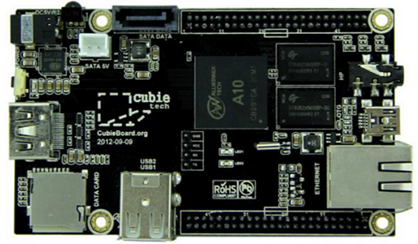
\includegraphics[width=0.45\textwidth]{obrazky/embed_cubie_1}\label{embed_cubie_1}}
			\hspace*{5mm}
			\subfigure[UpBoard 1]{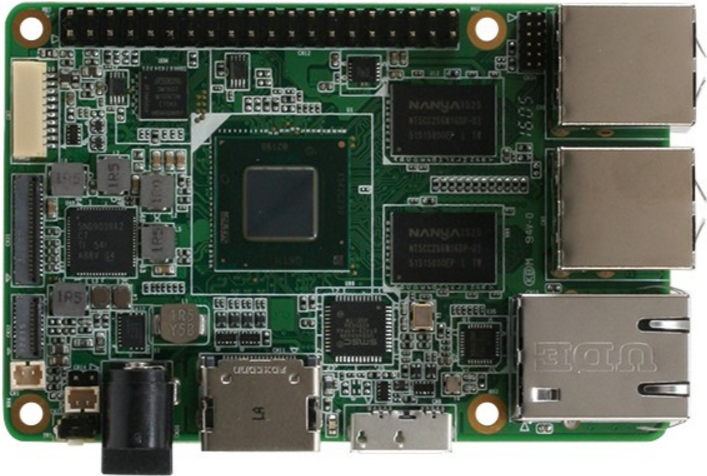
\includegraphics[width=0.45\textwidth]{obrazky/embed_upboard}\label{embed_upboard}}
			\caption{Cubieboard1 a UpBoard 1}
\end{figure*}
		

CubieBoardy již poskytují dostatečný výkon pro embeeded zařízení, přináší oproti RaspberryPi mnoho rozšiřujících sběrnic, avšak pro nedostatečnou podporu či zastoupení v evropských zemí a velmi častou nedostupnost webu výrobce, včetně dostupnosti anglické dokumentace pro  programování jednotlivých rozhraní, není moc vhodná pro IoT. Hodí se spíše pro aplikace jako multimediální centrum či nízkokládový počítač. 	

%%% ======================================= UP BOARD ============================ %%%

\subsection{Up Board}
		Up Board představuje miniaturní jednodeskový počítač na platformě Intel s čtyřjádrovým procesorem Intel Atom. Vzhledově je velice podpobný RaspberryPi 3. 
		Tento počítač obsahuje čtyřjádrový procesor Intel Atom x5-Z8300 na frekvenci 1,84 GHz s SDP 2\,W. Obsahuje 1\,GB RAM a 16\,GB flash eMMC (Embedded MultiMedia Card). 40 pinové rozhraní je totožné jako u RaspberryPi2 s níž je částečně kompatibilní. Navíc obsahuje gigabitový ethernetport, 5 USB 2.0 a jedno USB 3.0. Čip má hardwarovou podporu šifrování AES (Advanced Encryption Standard), je tedy vhodný pro IoT projekty s vyšším zabezpečením. Podporuje Android 5.0, Linux či Windows 10. Dokumentace pro programování GPIO v současnosti neexistuje a dokumentaci tvoří pouze popis GPIO konektoru~\cite{UpBoard}.

%%% ======================================= PINE64 ============================== %%%
	\subsection{PINE64}
Pine64 je rodina tří jednodeskových počítačů společnosti PINE64. Tyto počítače byly navrženy tak, aby konkurovali RaspberryPi ve výkonu a ceně. Všechny verze obsahují 64bitový čtyřjádrový procesor 1.152 GHz Cortex-A53 a liší se pouze velikostí operační paměti a použitelným operačním systémem. Oproti RaspberryPi obsahují gigabitový ethernet, wifi, bluetooth, port pro připojení dotykového panelu. Mají GPIO konektor shodný s danou verzi Raspberry, jsou s ní tedy do jisté míry kompatibilní. Zvlášností těchto desek je Eulerova sběrnice, která navyšuje počty sběrnic SPI, UART, GPIO~\cite{Pine64}.

\textbf{PINE A64 512MB} má 512\,MB paměti a podporuje pouze Arch Linux a Debian Linux.

\textbf{PINE A64+ 1GB} má 1\,GB paměti a podporuje i Android, Remix OS, Ubuntu a Windows IoT.

\textbf{PINE A64+ 2GB} má oproti předchozí verzi 2\,GB paměti.

	\begin{figure*}[!ht]
    \centering
			\subfigure[PINE A64+ 2GB]{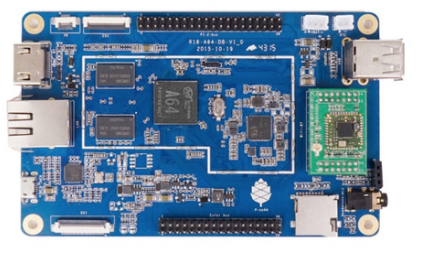
\includegraphics[width=0.45\textwidth]{obrazky/embed_pine}\label{embed_pine}}
			\hspace*{5mm}
			\subfigure[HardKernel Odroid-C2]{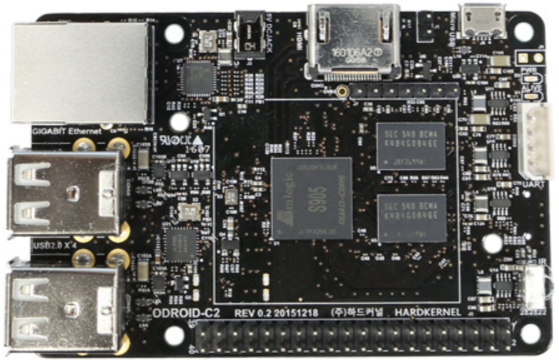
\includegraphics[width=0.45\textwidth]{obrazky/embed_odroidc2}\label{embed_odroidc2}}
			\caption{PINE A64+ 2GB a HardKernel Odroid-C2}
\end{figure*}

%%% ======================================= ODROID ============================== %%%
\subsection{HardKernel Odroid}
	\label{KapKernel}
ODROID je řada jednodeskových počítačů od společnosti Hardkernel. Název je odvozen z \textbf{O}pen An\textbf{droid}, ale podporovány jsou i linuxové distribuce. Desky disponují 40 pinovým GPIO kompatibilním s RaspberryPi, ale open-source již nejsou. Desky jsou postaveny na SoC platformě Samsung Exynos. Zvláštností desek je sériové rozhraní s 1.8\,V~\cite{HardKernel}.
	
	\textbf{ODROID-C1} je reakcí na RaspBerryPi 1. Nabídne čtyřjádrové SoC Cortex A5 s frekvencí 1,5\,GHz a 1\,GB RAM. Dále má gigabitový Ethernet a připojení flash úložiště typu eMMC. 

	\textbf{ODROID-C2} je reakcí na RaspberryPi 3. Obsahuje čtyřjádrový 64bitový procesor ARMv8 taktovaný na 2\,GHz, 2\,GB paměti a gigabitový ethernet. Má podporu sběrnice I2S. Hlavní změnou je podpora HDMI 2.0 a schopností přehrávat 4K video ve formátu H.265. Podporuje Ubuntu 16.04 nebo Android 5.1. 
	
	\textbf{ODROID-XU4} je výkonejší řada desek, obsahují čtyřjádrový procesor Samsung Exynos5 ARM Cortex-A15 na frekvenci 2\,GHz a čtyřjádrový procesor Cortex-A7 Quad 1.3\,GHz, bohužel vzhledem k výkonu je zde již potřeba aktivní chlazení. Deska disponuje grafickým čipem Mali-T628 MP6 a 2\,GB RAM paměti.

	
%%% ======================================= BeagleBoard ============================== %%%
\subsection{BeagleBoard }
BeagleBoard je skupina jednodeskových počítačů produkovaných společností Texas Instruments, navržených na čipu Texas Instrument's OMAP3530 SoC, ten obsahuje ARM Cortex-A8 CPU, který může provozovat Linuxové distribuce, BSD nebo Android. Desky obsahují dva 46pinové GPIO konektory, oproti ostatním přináší podporu CAN (Controller Area Network) sběrnice. Výrobce poskytuje vlastní řadu komptibilních rozšiujících desek, nazýva je \uv{capes} a současně lze připojit až 4 takovéto desky. Výhodou desek je jejich nízká spotřeba, využívají až 2 W elektrické energie a mohou být napájeny i ze samostatného napájení. Vzhledem k nízké spotřebě energie, nejsou nutné žádné přídavné chladiče~\cite{BeagleBone}.

\textbf{BeagleBoard} obsahuje procesor Sitara ARM Cortex-A8 na frekvenci 720\,MHz a disponuje dle revize 128 nebo 256\,MB RAM. Obsahuje 256\,MB NAND paměti.

\textbf{BeagleBone} obsahuje procesor Sitara ARM Cortex-A8 na frekvenci 720\,MHz a disponuje 256\,MB RAM.

\textbf{BeagleBoard-X15} je založen na procesoru Sitara AM5728 s dvěma jádry ARM Cortex-A15 na frekvenci 1,5\,GHz a dvěma jádry ARM Cortex-M4 na frekvenci 212\,MHz and dvěma jádry TI C66x DSP na frekvenci 700\,MHz. Disponuje 2\,GB RAM. Použitý procesor přináší podporu HDMI 3.0, gigabit Ethernetu a grafického dvoujádrového čipu SGX544 na frekvenci 532\,MHz. 

	\begin{figure}[!ht]
  \begin{center}
    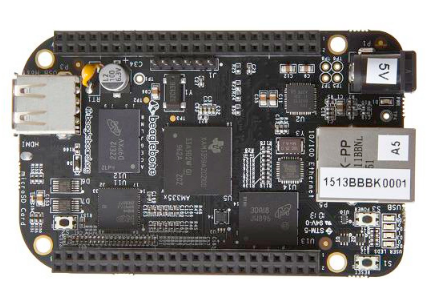
\includegraphics[scale=0.7]{obrazky/embed_beaglebone_black}
  \end{center}
  \caption{BeagleBone Black~\cite{BeagleBone}}
\end{figure}

\textbf{BeagleBone Black} má oproti předchůdci zvýšenou pamět na 512\,MB, frekvenci procesoru na 1\,GHz, bylo přidáno HDMI a 2\,GB eMMC flash paměti.

%%%%%%%%%%%%%%%%%%%%%%%%%%%%%%%%%%%%%%%%%%%%%%%%%%%%%%%%%%%%%%%%%%%%%%%%%%%%%%%%%%%%%%%%%%%%%%%%%%%%%%%%%%%%%%%%%
%%%%%%%%%%%%%%%%%%%%%%%%%%%%%%%%%%%%%%%%%%%%%%%%%%%%%%%%%%%%%%%%%%%%%%%%%%%%%%%%%%%%%%%%%%%%%%%%%%%%%%%%%%%%%%%%%
%%%%%%%%%%%%%%%%%%%%%%%%%%%%%%%%%%%%%%%%%%%%%%%%%%%%%%%%%%%%%%%%%%%%%%%%%%%%%%%%%%%%%%%%%%%%%%%%%%%%%%%%%%%%%%%%%
%%%%%%%%%%%%%%%%%%%%%%%%%%%%%%%%%%%%%%%%%%%%%%%%%%%%%%%%%%%%%%%%%%%%%%%%%%%%%%%%%%%%%%%%%%%%%%%%%%%%%%%%%%%%%%%%%
%%%%%%%%%%%%%%%%%%%%%%%%%%%%%%%%%%%%%%%%%%%%%%%%%%%%%%%%%%%%%%%%%%%%%%%%%%%%%%%%%%%%%%%%%%%%%%%%%%%%%%%%%%%%%%%%%
%%%%%%%%%%%%%%%%%%%%%%%%%%%%%%%%%%%%%%%%%%%%%%%%%%%%%%%%%%%%%%%%%%%%%%%%%%%%%%%%%%%%%%%%%%%%%%%%%%%%%%%%%%%%%%%%%

\section{Intel}
\label{KapIntel}

Společnosti Intel přináší dva jednodeskové počítače založené na platformě mikroprocesoru x86. Jsou navrženy jak pro vývojáře tak k výuce výpočetní techniky.

		\subsection{Intel Galileo}
		Intel Galileo je jednočipový počítač, vyvinutý společností Intel, postavený na architektuře x86. Obsahuje procesor Intel Quark x86 na frekvenci 400\,MHz. Má 256\,MB RAM. Byl navržen pro výuku výpočetní techniky. Jedná se o první zařízení od Intelu, které je hardwarově i softwarově kompatibilní s Arduinem. Lze k němu připojovat Arduino shieldy i moduly a využívat vývojové prostředí Arduina, včetně jeho knihoven. 
		Tento počítač obsahuje 14 digiálních I/O pinů, z toho 6 z nich lze využít jako PWM výstupy. Dále obsahuje 6 analogových vstupů, UART sběrnici, I2C sběrnici, SPI sběrnici, Ethernet konektor, slot na MicroSD kartu. Dále obsahuje 2 USB konektory, jeden USB-host, druhý USB-klient. Druhá generace této desky pak přináší podporu PoE (Power over Ethernet)a další drobné změny~\cite{IntelGalileo,ArduinoGalileo}.
\begin{figure}[!ht]
  \begin{center}
    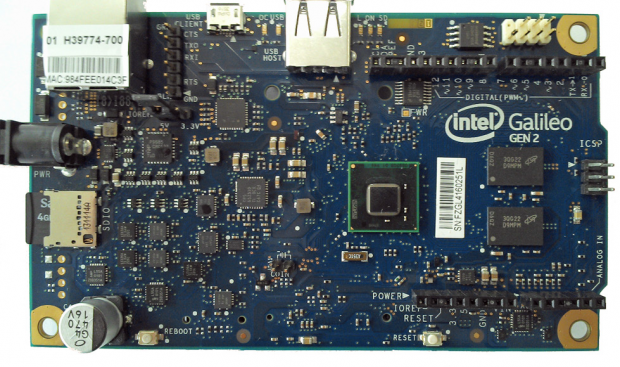
\includegraphics[scale=0.45]{obrazky/embed_intel_galileo}
  \end{center}
  \caption{Intel Galileo~\cite{IntelGalileo}}
\end{figure}
		
		
		\subsection{Intel Edison} 
		Intel Edison je druhý jednočipový počítač architektury x86 vyvinutý společností Intel. Má velikost SD karty a je určený pro nositelnou elektroniku. Obsahuje dvoujádrový procesor Intel Quark x86 na frekvenci 400 MHz. Dále obsahuje 1\,GB RAM a 4\,GB flash paměti. Konektivita je zajištěna pomocí 70 pinového Hirose DF40 konektoru, který v sobě sdružuje veškerá dostupná rozhraní (USB, GPIO, SPI, I2C a PWM). Jsou k dispozici dvě rozšiřující desky~\cite{IntelEdison}:
			
			\begin{itemize}
				\item Arduino board - Arduino board je plně kompatibilní s Arduinem, včetně podpory Arduino shieldů a modulů. Dále tato deska zpřístupňuje 20 digiálních I/O pinů, z toho 4 z nich lze využít jako PWM výstupy. Dále obsahuje 6 analogových vstupů, UART sběrnici, I2C sběrnici, SPI sběrnici. Dále obsahuje 2 USB konektory, jeden pro napájení, druhý připojený k UART sběrnici a slot na SD kartu.
				\item Intel breakout board -  Tato deska je díky svým malým rozměrům vhodná pro prototypování nositelné elektroniky či pro Internet věcí. Obsahuje pájitelnou mřížku pro zpřístupnění věškerých dostupých rozhraní. Na desku jsou vyvedeny pouze dva USB konektory, jeden pro napájení a druhý připojený k UART sběrnici.
\end{itemize}


\begin{figure*}[!ht]
    \centering
			\subfigure[Arduino board]{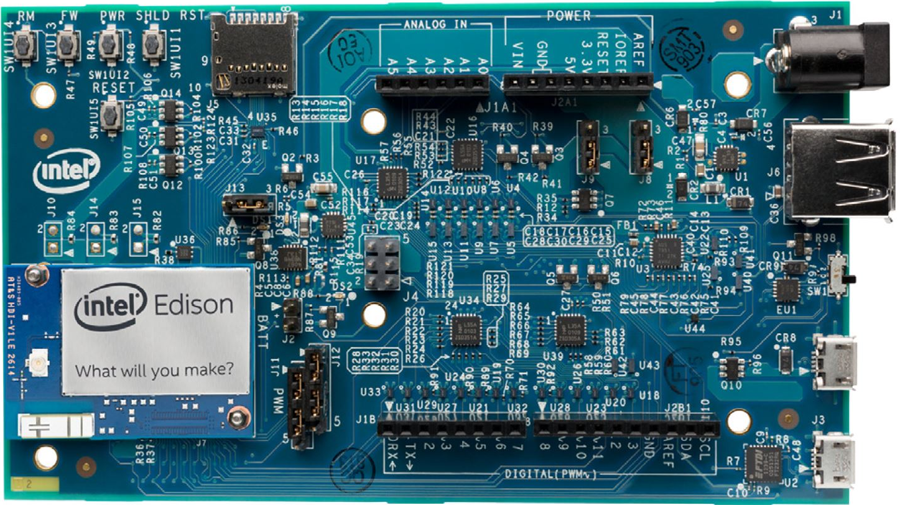
\includegraphics[width=0.45\textwidth]{obrazky/embed_intel_edison2}\label{embed_intel_edison2}}
			\hspace*{5mm}
			\subfigure[Intel breakout board]{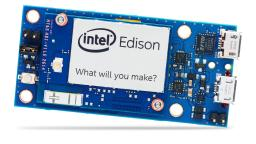
\includegraphics[width=0.45\textwidth]{obrazky/embed_intel_edison1}\label{embed_intel_edison1}}
		\caption{Intel Edison zasazeny na boardech}
\end{figure*}
	

Desky Intel se hodí spíše pro větší typy projektů, kdy již vývojové prostředí Arduina nestačí a je potřeba využít plného potencálu operačního systému.

%%%%%%%%%%%%%%%%%%%%%%%%%%%%%%%%%%%%%%%%%%%%%%%%%%%%%%%%%%%%%%%%%%%%%%%%%%%%%%%%%%%%%%%%%%%%%%%%%%%%%%%%%%%%%%%%%
%%%%%%%%%%%%%%%%%%%%%%%%%%%%%%%%%%%%%%%%%%%%%%%%%%%%%%%%%%%%%%%%%%%%%%%%%%%%%%%%%%%%%%%%%%%%%%%%%%%%%%%%%%%%%%%%%
%%%%%%%%%%%%%%%%%%%%%%%%%%%%%%%%%%%%%%%%%%%%%%%%%%%%%%%%%%%%%%%%%%%%%%%%%%%%%%%%%%%%%%%%%%%%%%%%%%%%%%%%%%%%%%%%%
%%%%%%%%%%%%%%%%%%%%%%%%%%%%%%%%%%%%%%%%%%%%%%%%%%%%%%%%%%%%%%%%%%%%%%%%%%%%%%%%%%%%%%%%%%%%%%%%%%%%%%%%%%%%%%%%%
%%%%%%%%%%%%%%%%%%%%%%%%%%%%%%%%%%%%%%%%%%%%%%%%%%%%%%%%%%%%%%%%%%%%%%%%%%%%%%%%%%%%%%%%%%%%%%%%%%%%%%%%%%%%%%%%%
%%%%%%%%%%%%%%%%%%%%%%%%%%%%%%%%%%%%%%%%%%%%%%%%%%%%%%%%%%%%%%%%%%%%%%%%%%%%%%%%%%%%%%%%%%%%%%%%%%%%%%%%%%%%%%%%%

 \section{AMD Gizmo}
\label{KapAMD}

	Gizmo Board a Gizmo Board 2 od firmy AMD jsou alternativou k počítačům RaspberryPi, nabízející však platformu IBM PC a plně 64bitovou architekturu. Umožňuje tedy běh klasických operačních systémů, včetně Windows.
	
		\textbf{Gizmo Board 1} beží dvoujádrovém APU G-T40E od firmy AMD, běžíci na frekvenci 1GHz při příkonu 10\,W. Součástí procesoru je grafický čip Radeon HD 6250. K dispozici je 1\,GB RAM. Deska dále obsahuje dvojici USB, VGA, audio výstup, SATA a ethernet konektor. Další sběrnice jako GPIO, SPI, I2C, UART a PWM jsou dostupné po připojení rozšiřující karty přes LowSpeed~\cite{AmdGizmo1}.
	
	\textbf{ Gizmo Board 2} je vybaven APU AMD GX210HA na frekvenci 1 GHz, s integrovaným GPU AMD Radeon HD 8210E s frekvencí 300\,MHz. Příkon je 9\,W. Tento model má také 1\,GB RAM. tato verze disponuje 4 USB, HDMI výstupem, MicroSD slotem a ethernetovým portem. Mezi další rozhraní patří PCI Express (Peripheral Component Interconnect Express), GPIO, SPI, I2C, UART, DAC/ADC nebo PWM \cite{AmdGizmo2}.


	\newpage

\begin{figure*}[!ht]
    \centering
			\subfigure[Gizmo Board 1]{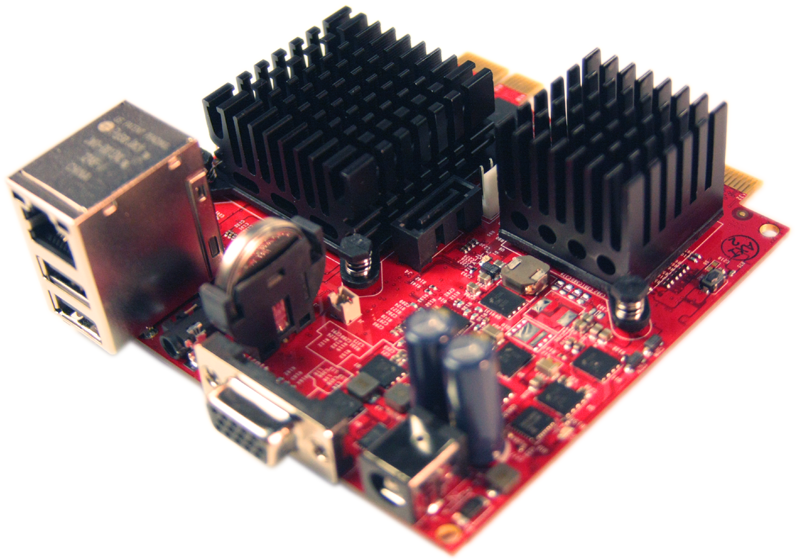
\includegraphics[width=0.45\textwidth]{obrazky/embed_amd_gizmo1}\label{embed_amd_gizmo1}}
			\hspace*{5mm}
			\subfigure[Gizmo Board 2]{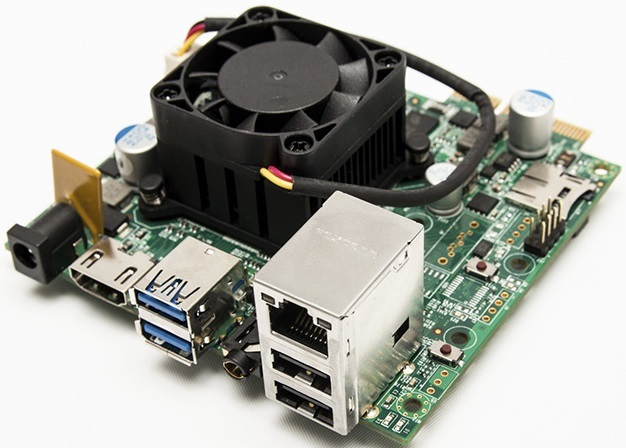
\includegraphics[width=0.45\textwidth]{obrazky/embed_amd_gizmo2}\label{embed_amd_gizmo2}}
		\caption{AMD Gizmo}
\end{figure*}



	
Oba počítače již poskytují dostatečný výkon pro embeeded zařízení, avšak oba již využívají aktivní chlazení, jsou hlučnější, větších rozměrů a nemají dostatečnou dokumentaci k přístupu a programování jednotlivých rozhraní. Hodí se spíše pro aplikace jako multimediální centrum či jednodušší počítač, než pro IoT nebo průmyslovou automatizaci. Komunita okolo AMD Gizmo prakticky neexistuje.
	
	





%% Vložení kapitoly o UniPi
\chapter{Rozšiřující deska UniPi}
\label{KapUnipi}

UniPi je česká firma, nyní dceřiná společnost Faster.cz, původně její oddělení měření a regulace, které se zaměřuje na inteligentní stavební řešení, domácí automatizaci a~Internet věcí. Dále provozuje výzkum a vývoj rozšiřujicích desek UniPi, včetně jejich softwarového vybavení \cite{UniPi}.

UniPi je taktéž pojmenování pro přídavné rozšiřující desky pro RaspberryPi, se~kterou je plně kompatibilní ve všech verzích. Je vybavena řadou komponent, jako jsou například digitální galvanicky oddělené vstupy s LED signalizací, 0\,-\,10\,V analogové vstupy, 0\,-\,10\,V analogové výstupy, spínací relé, jednokanálová 1Wire sběrnice, I2C sběrnice, UART sběrnice, SPI sběrnice a RS-485 sběrnice.

UniPi je název, odvozený od slov \uv{RaspberryPi} a \uv{univerzální}, protože jednoduchost a univerzálnost jsou základní charakteristiky této desky. Deska původně vznikla pro potřeby řízení energetických hodnot vlastního datacentra Zelená Data \cite{ZelenaData}, ale škála odvětví, kde je možné UniPi nasadit je rozsáhlá, pro představu výrobce uvádí několik příkladů \cite{UniPi}:
\begin{itemize}
	\item Docházkové a přístupové systémy.
	\item Bezpečnostní systémy.
	\item Topné, chladící prvky i řízení.
	\item Větrání, rekuperace.
	\item Řídící systémy, které nejsou kompletní.
	\item Dohledové systémy.
	\item Ovládání světelných prvků.
	\item Datové vypínače.
	\item Řízení pivovarnických technologií.
	\item Zavlažovací systémy.
	\item Wellness systémy – vířivé vany, bazény, sauny.
	\item Solární systémy.
\end{itemize}

\vspace{5mm}
\noindent
 V současnosti existují dvě verze rozšiřující desky UniPi:


\begin{itemize}
	\item UniPi (verze 1)\footnote[1]{Dostupné z: \href{http://unipi.technology/product/unipi/}{http://unipi.technology/product/unipi/}}.
	\item UniPi Neuron (verze 2)\footnote[2]{Dostupné z: \href{http://unipi.technology/product/unipi-neuron-s103/}{http://unipi.technology/product/unipi-neuron-s103/}}.
\end{itemize}

\vspace{5mm}
Desky se liší svými vstupně-výstupními možnostmi, rozměry a jsou dostupné v několika variantách.



%%%%%%%%%%%%%%%%%%%%%%%%%%%%%%%%%%%%%%%
%%%%%%%%%%%%%%%%%%%%%%%%%%%%%%%%%%%%%%%
%%%%%%%%%%%%%%%%%%%%%%%%%%%%%%%%%%%%%%%

\section{UniPi v1}
\label{KapitolaUnipi1}

Deska UniPi je prezentována jako nejlevnější a nejjednodušší řešení pro inteligentní budovy a IoT. Je navržena pro maximální kompatibilitu s embedded zařízením RaspberryPi. Zařízení bylo vyvinuto primárně jako rozhraní pro příjem vstupních signálů, jejich vyhodnocení a~realizaci výstupní reakce na základě naprogramovaných algoritmů \cite{UniPiBoard1}.

Disponuje (viz Obr.~\ref{ObrazekUnipiV1}) osmi relé pro střídavý proud, čtrnácti digitálními vstupy, jedním jednokanálovým 1Wire rozhraním, dvěma 0\,-\,10\,V analogovými vstupy a jedním 0\,-\,10\,V analogovým výstupem. Zajímavou součástí desky je také modul reálného času. Druhý I2C port na RaspberryPi v sobě navíc ukrývá 5\,V měnič napětí a ochranu ESD (ElectroStatic Discharge), umožňující tak připojení dalších zařízení. Pro jednoduché připojení jednotlivých sběrnic jsou na desce umístěny konektory.

 \begin{figure}[!ht]
  \begin{center}
    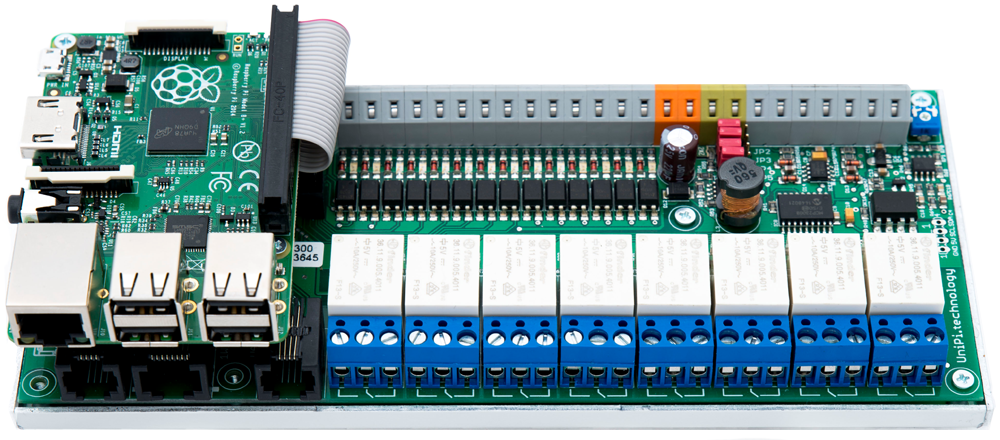
\includegraphics[scale=0.75]{obrazky/unipi_v1}
  \end{center}
	\vspace{-20pt}
  \caption{Popis UniPi v1 \cite{UniPiBoard1}}
	\label{ObrazekUnipiV1}
	\vspace{-30pt}
\end{figure}

\subsubsection{Popis desky}
\begin{itemize}
	\item 14 digitálních vstupů 5\,–\,24\,V. 
	\item 1Wire sběrnice pro měření teploty a vlhkosti. 
	\item 8 přepínacích relé 250\,V/5\,A AC nebo 24\,V/5\,A DC.
	\item 1 Analogový výstup 0\,–\,10\,V.
	\item 2 Analogové vstupy 0\,–\,10\,V.
	\item Modul reálného času.
	\item I2C sběrnice.
	\item EEPROM paměť.
	\item UART sběrnice.
	\item Notifikační diody pro zobrazení stavu jednotlivých portů.
\end{itemize}

\vspace{10pt}
Velkou výhodou řídicí jednotky UniPi je zabudovaný čip pro obsluhu teplotních čidel na sběrnici 1Wire. Digitální teploměry mají svou adresu, není tedy nutné je~jakkoliv kalibrovat či nastavovat, stačí zapojit.

S RaspberryPi je deska UniPi propojena 26\,žilovým kabelem přes GPIO konektor. Jak bylo popsáno v kapitole~\ref{KapGPIO} o konektoru GPIO, toto propojení je z důvodu kompatibility shodné pro všechny verze RaspberryPi. Vnitřní uspořádání desky je~řešeno pomocí funkčních celků  (znázorněno na Obr.~\ref{SchemaBlok1}), které jsou propojeny pomocí I2C sběrnice. Výstupy jednotlivých celků jsou poté vyvedeny na konektory desky.
 
\begin{figure}[!ht]
\vspace{-20pt}
  \begin{center}
    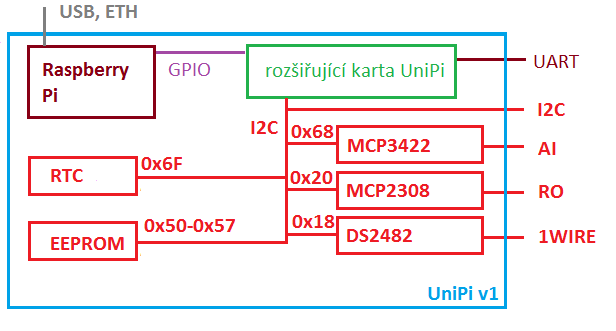
\includegraphics[scale=0.85]{obrazky/unipi_schema1}
  \end{center}
	\vspace{-30pt}
  \caption{Blokové schéma UniPi v1}
	\label{SchemaBlok1}
	
\end{figure}

Napájení desky je řízeno jumperem JP1 a může být řešeno dvěma způsoby:
\begin{itemize}
	\item Adaptérem 5\,V/2\,A do UniPi, s distribucí 5\,V/750\,mA do RaspberryPi.
	\item Samostatným nápajením obou desek.
\end{itemize}

\vspace{10pt}
Pro účely testování a implementace byla zapůjčena deska UniPi s počítačem RaspberryPi 2. Vývoj této desky byl již ukončen a nahrazen druhou verzí, označovanou jako UniPi NEURON.



%%%%%%%%%%%%%%%%%%%%%%%%%%%%%%%%%%%%%%%
%%%%%%%%%%%%%%%%%%%%%%%%%%%%%%%%%%%%%%%
%%%%%%%%%%%%%%%%%%%%%%%%%%%%%%%%%%%%%%%

\section{UniPi v2 - Neuron}
\label{KapitolaUnipi2}

UniPi Neuron představuje modulární PLC (Programmable Logic Controller) pro chytrou domácnost a inteligentní systémy budov, řízení a průmyslovou automatizaci. Díky modulární a kompaktní konstrukci nabízí jedinečnou variabilitu funkcí. UniPi Neuron je univerzální řídící jednotka. Neuron lze použít k řízení chytrého domu nebo jako domácí server. Je vhodný pro monitorování, sběr a ukládání dat na vzdálený server, nebo jako výkonná a plně vybavená brána pro ostatní zařízení \cite{UniPiBoard2}.

 \begin{figure}[!ht]
  \vspace{-30pt}
  \begin{center}
    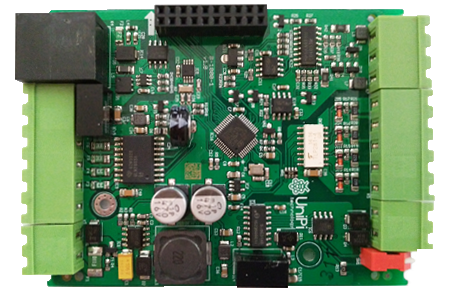
\includegraphics[scale=0.25]{obrazky/unipi_unipi_deska}
  \end{center}
	\vspace{-20pt}
  \caption{UniPi rozšiřující deska}
	\label{UnipiV2DeskaUnipi}
	\vspace{-10pt}
\end{figure}

UniPi Neuron je na rozdíl od první verze, kdy se rozšiřujicí deska RaspberryPi distribuovala zvlášt, již hotové řešení, které se skládá z RaspberryPi, rozšiřující desky UniPi verze 2 (viz Obr.~\ref{UnipiV2DeskaUnipi}), propojovací desky pro komunikační moduly (viz Obr.~\ref{unipi_osazeny}) a diodového panelu. To vše propojené a uzavřené v modrém plechovém pouzdru s možností montáže na DIN lištu. K dostání je tedy pouze jako hotový výrobek.


\subsubsection{Popis desky}
\begin{itemize}
\item Digitalní vstup 4\,-\,24\,V (počet závislý na konkrétním modelu).
\item Tranzistorový výstup 50V/750 mA (počet závislý na konkrétním modelu).
\item Analogový výstup 0\,-\,10\,V.
\item Analogový vstup 0\,-\,10\,V.
\item 1Wire sběrnice.
\item RS-485 .
\item Modul reálného času.
\item Notifikační diody pro zobrazení stavu jednotlivých portů.
\end{itemize}

\vspace{10pt}
UniPi Neuron existuje v několika verzích (viz Obr.~\ref{UnipiNeuronModels}), rozlišených počtem digitálních vstupů a výstupů, parametrů procesoru a velikosti paměti RAM. Do budoucna by měly být také k dostání verze s jedním konkrétním modulem (Wireless M-Bus, ZigBee, GPRS, \ldots) uvnitř.

\begin{figure*}[!ht]
    \centering
			\subfigure[S103]{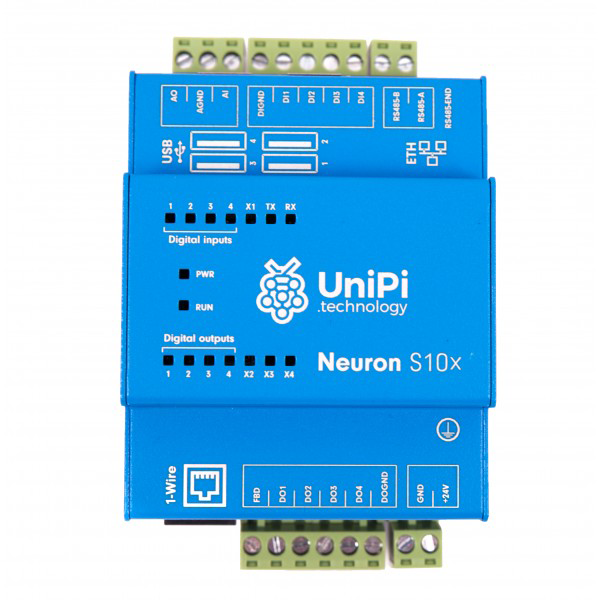
\includegraphics[width=0.3\textwidth]{obrazky/unipi_neuron_s}\label{unipi_neuron_s}}
			\hspace*{5mm}
			\subfigure[M203]{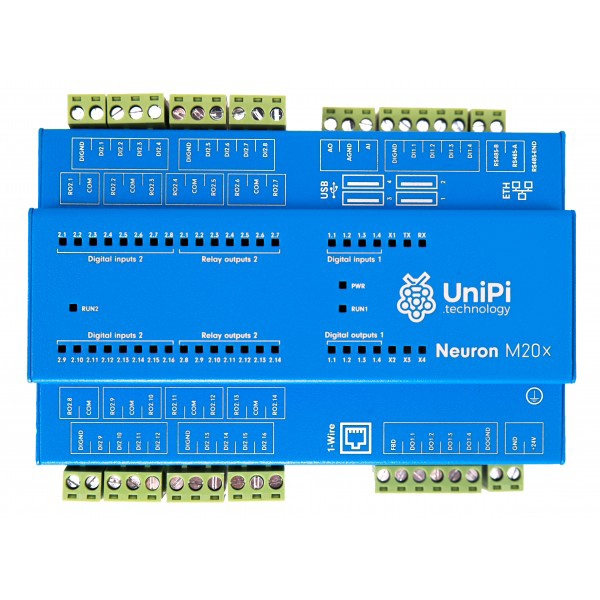
\includegraphics[width=0.3\textwidth]{obrazky/unipi_neuron_m}\label{unipi_neuron_m}}
			\hspace*{5mm}
			\subfigure[L303]{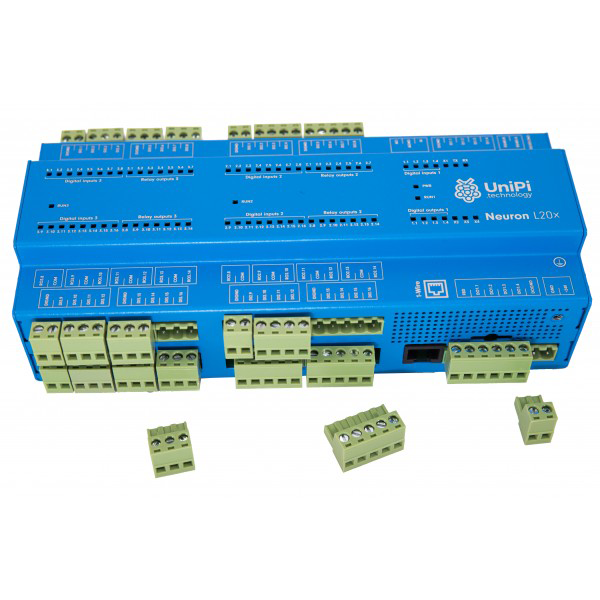
\includegraphics[width=0.3\textwidth]{obrazky/unipi_neuron_l}\label{unipi_neuron_l}}
			\caption{Unipi Neuron~\cite{UniPiBoard2}}
			\label{UnipiNeuronModels}
\end{figure*}

\vspace{10pt}
Standardní modely NEURON mají proměnlivé množství digitálních vstupů a~reléových výstupů. Jejich počet je uveden v Tab.~\ref{TableUnipiIO}.

\begin{table}[!ht]
\caption{Porovnání modelů UniPi NEURON dle I/O \cite{UniPiBoard2}}
\vspace{-20pt}
\label{TableUnipiIO}
	\begin{center}
	\resizebox{\textwidth}{!}{%
	\begin{tabular}{|l|c|c|c|}
		\hline
		\textbf{Model} & \multicolumn{1}{l|}{\textbf{\begin{tabular}[c]{@{}l@{}}Počet digitálních vstupů\end{tabular}}} & \multicolumn{1}{l|}{\textbf{\begin{tabular}[c]{@{}l@{}}Počet digitálních výstupů\end{tabular}}} & \multicolumn{1}{l|}{\textbf{\begin{tabular}[c]{@{}l@{}}Velikost na DIN liště\end{tabular}}} \\ \hline \hline
		\textbf{S10x} & 4 & 0 & 4 moduly \\ \hline
		\textbf{M10x} & 12 & 8 & 8 modulů \\ \hline
		\textbf{M20x} & 20 & 14 & 8 modulů \\ \hline
		\textbf{M30x} & 34 & 0 & 8 modulů \\ \hline
		\textbf{M40x} & 4 & 28 & 8 modulů \\ \hline
		\textbf{L20x} & 36 & 28 & 12 modulů \\ \hline
		\textbf{L30x} & 64 & 0 & 12 modulů \\ \hline
		\textbf{L40x} & 4 & 56 & 12 modulů \\ \hline \hline
	\end{tabular}}
	\end{center}
\end{table}

\newpage
Písmeno x v Tab.~\ref{TableUnipiVar} bývá nahrazeno číslem 1-3 dle osazeného typu RaspberryPi:

\begin{table}[!ht]
\caption{Varianty modelů UniPi NEURON dle CPU a RAM \cite{UniPiBoard2}}
\vspace{-10pt}
\label{TableUnipiVar}
	\begin{center}
\begin{tabular}{|c|c|c|c|c|}
\hline
x & \textbf{Osazená deska} & \textbf{CPU} & \textbf{RAM} & \textbf{Další vlastnosti} \\ \hline \hline
\textbf{1} & RaspberryPi B+ & 700\,MHz & 512\,MB &  \\ \hline
\textbf{2} & RaspberryPi 2 & 4\,x\,900\,MHz & 1\,GB &  \\ \hline
\textbf{3} & RaspberryPi 3 & 4\,x\,1200\,MHz & 1\,GB & BT 4.1, WiFi 802.11n \\ \hline \hline
\end{tabular}
	\end{center}
\end{table}

\newpage

S RaspberryPi je deska UniPi propojena, obdobně jako u první verze, pomocí 26 pinové desky propoující GPIO port na RaspberryPi s konektorem na rozšiřující desce UniPi. Na samotné propojující desce (viz Obr.~\ref{unipi_propojbrain}) je vyvedena UART a~I2C sběrnice. 

\begin{figure*}[!ht]
		\vspace{-10pt}
    \centering
			\subfigure[Propojení desek]{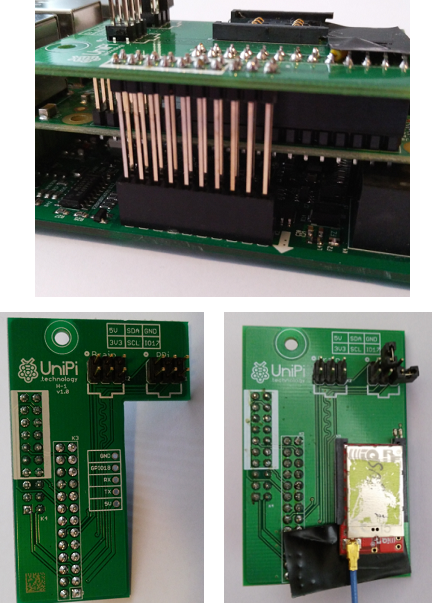
\includegraphics[width=0.45\textwidth]{obrazky/unipi_propojbrain}\label{unipi_propojbrain}}
			\hspace*{5mm}
			\subfigure[UniPi deska osazená WM-Bus modulem]{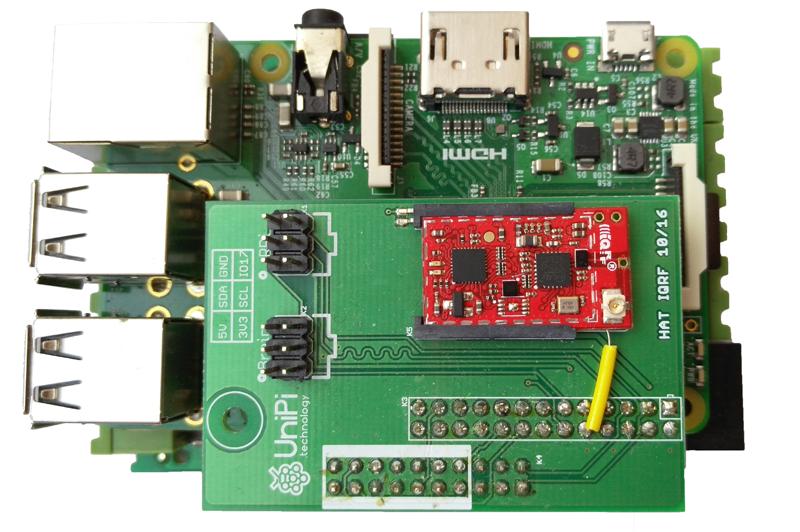
\includegraphics[width=0.45\textwidth]{obrazky/unipi_osazeny}\label{unipi_osazeny}}
			\caption{Detaily UNiPi desky}
			\vspace{-5pt}
\end{figure*}

Na I2C sběrnici je dále připojen panel (viz Obr.~\ref{unipi_propojuvnitr}) se signalizačními diodami. UART sběrnice je zde připravena pro připojenů dalších modulů. Tyto desky jsou k~dostání v několika verzích, přizpůsobené konektorem pro konkrétní komunikační modul. Deska na obrázku~\ref{unipi_osazeny} je osazena WM-Bus modulem.
 
Celá sestava desek je poté uložena v kovové krabičce s označením vstupů a výstupů (viz Obr.~\ref{unipi_unipi_box}).


\begin{figure*}[!ht]
		\centering
			\subfigure[Uložení v krabičce]{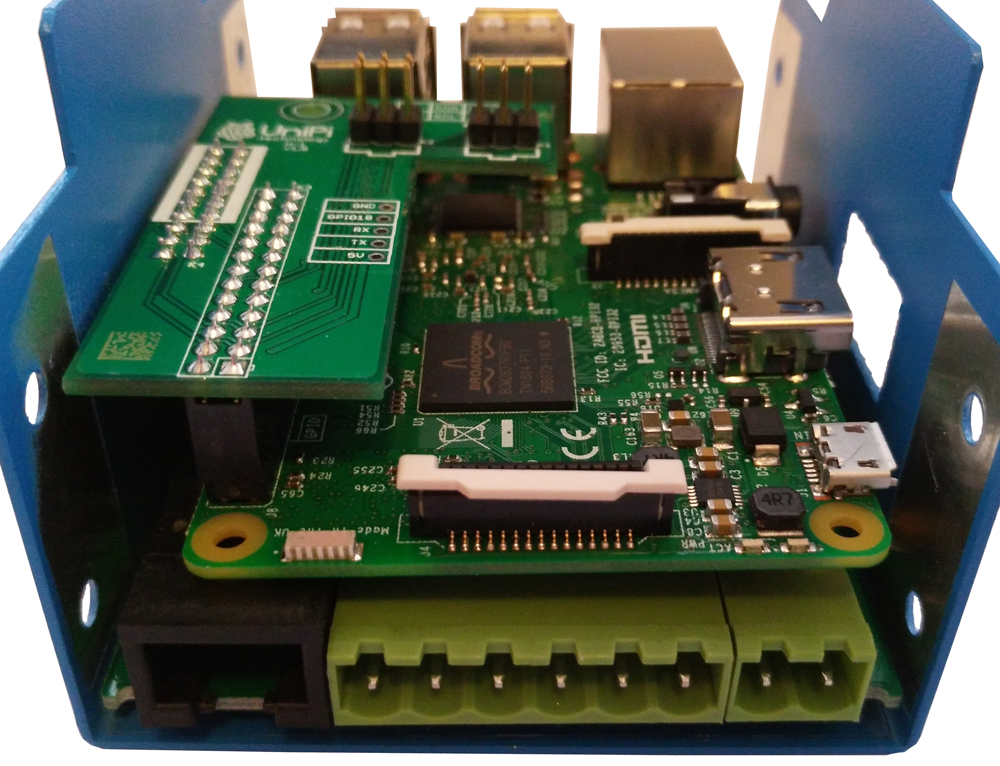
\includegraphics[width=0.45\textwidth]{obrazky/unipi_unipi_box}\label{unipi_unipi_box}}
			\hspace*{5mm}
			\subfigure[Připojení diodového panelu]{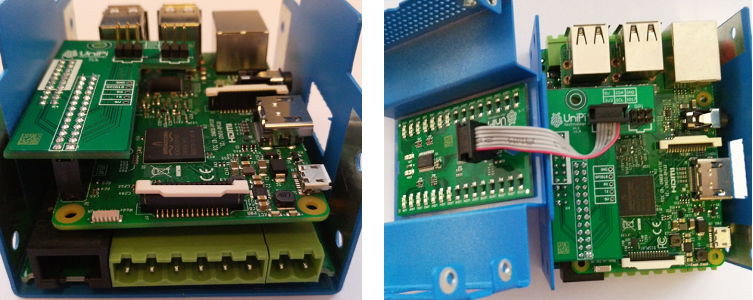
\includegraphics[width=0.45\textwidth]{obrazky/unipi_propojuvnitr}\label{unipi_propojuvnitr}}
			\caption{Detaily vnitřního uspořádání UniPi Neuronu S103}
			\vspace{-5pt}
\end{figure*}

Vnitřní uspořádání desky je řešeno pomocí funkčních celků (viz Obr.~\ref{BlokUniPi2Schema}), které jsou propojeny pomocí I2C sběrnice. Výstupy jednotlivých celků jsou poté vyvedeny na konektory desky.
 \begin{figure}[!ht]
	\vspace{-10pt}
  \begin{center}
    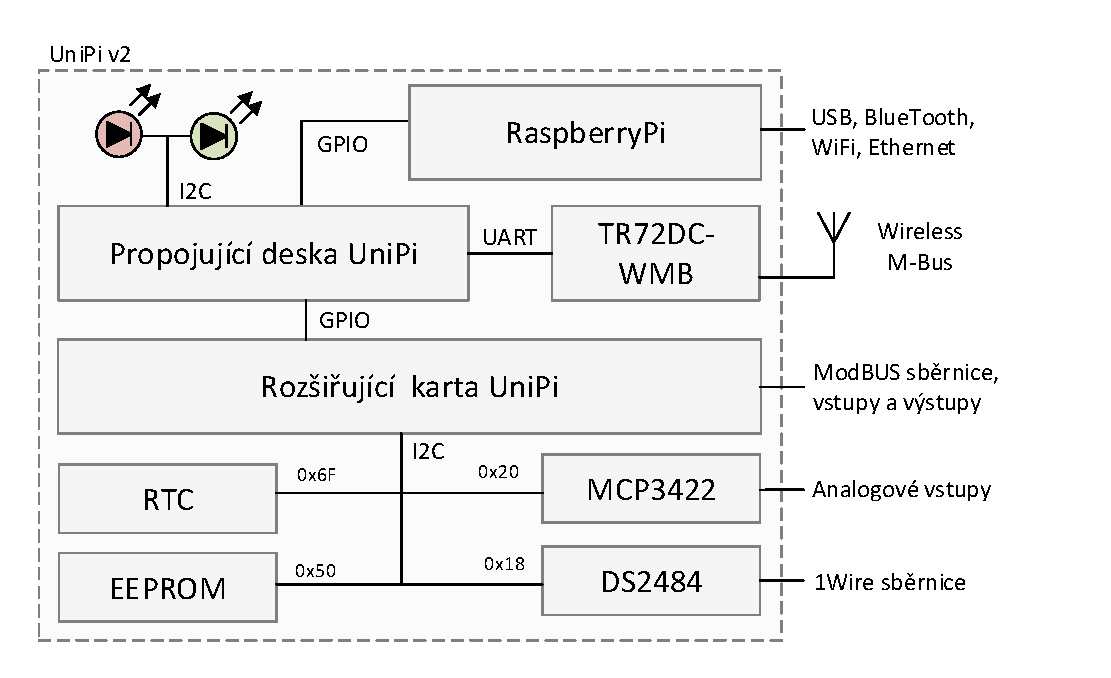
\includegraphics[scale=0.75]{obrazky/unipi_schema2}
  \end{center}
	\vspace{-30pt}
	\caption{Blokové schéma UniPi v2}
	\label{BlokUniPi2Schema}
	\vspace{-10pt}
\end{figure}

Napájení desky je pomocí 24\,V/1,5\,A adaptéru přímo na rozšiřující desku UniPi. Pro účely testování a implementace byla zapůjčena deska UniPi Neuron S103 vybavená počítačem RaspberryPi 3.

 %\begin{figure}[!h]
 % \begin{center}
 %   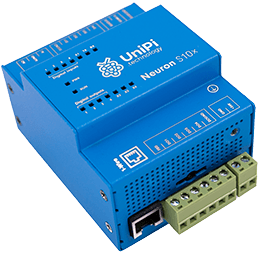
\includegraphics[scale=1.0]{obrazky/unipi_v2}
 % \end{center}
 % \caption{UniPi Neuron S10x (v2) [docasne prevzeti]}
%\end{figure}

%%%%%%%%%%%%%%%%%%%%%%%%%%%%%%%%%%%%%%%
%%%%%%%%%%%%%%%%%%%%%%%%%%%%%%%%%%%%%%%
%%%%%%%%%%%%%%%%%%%%%%%%%%%%%%%%%%%%%%%

\section{Srovnání obou verzí}

Jak bylo popsáno v předchozím textu (Kap.~\ref{KapitolaUnipi1}~a~\ref{KapitolaUnipi2}), obě verze UniPi se liší svými parametry a využitím. I když vývoj UniPi byl nahrazen vývojem UniPi NEURONu, stále se najdou aplikace vhodné pouze pro původní desku:


\begin{itemize}
	\item Deska UniPi má reléově spínané výstupy, lze pomocí ní spínat i silové výstupy do 250\,V. Zatímco UniPi NEURON má spínané tranzistorové výstupy pouze do 50\,V, pro spínání vyšších napětí je nutné připojit reléový modul.
	\item Deska UniPi má zpřístupněnou I2C a UART sběrnici, zatímco na UniPi Neuronu je I2C využita pouze pro adresování vnitřních bloků a UART sběrnice je~alokována pro rozšiřující komunikační moduly.
	\item Software EVOK a software postavené na něm jsou v tomto okamžiku plně funkční pouze na desce první verze.	
\end{itemize}

\vspace{10pt}
Na některé aplikace však již tato deska vhodná není a je lepší využít UniPi NEURON:

\begin{itemize}
	\item I když UniPi první verze má sběrnici UART a teoretecky do ní lze připojit stejné rozšiřující komunikační moduly jako do UniPi Neuronu, součástí vývoje budou jen rozšiřující desky pro UniPi NEURON, jejichž nabídka má obsahovat spoustu dostupných technologií.
	\item Vzhledem k rozsáhlé nabídce modelů UniPi NEURON lze zvolit řešení na míru, včetně další konektivity.
	\item UniPi NEURON disponuje sběrnici RS-485 s protokolem ModBUS.
	\item UniPi NEURON má na kontaktech vysouvací svorky a celý modul zabírá méně místa.	
\end{itemize}

\vspace{10pt}
Vzhledem k tomu, že UniPi NEURON je v době vypracování práce jediná vývojem podporovaná verze, bude implementaci WM-Bus protokolu provedena na této verzi, avšak lze bez jakýchkoliv softwarových modifikací a pouze s jednou hardwarovou modifikací implementovat WM-Bus protokol i na UniPi první verze. Stačí pouze propojit příslušné piny IQRF modulu s piny modulárního konektoru UART sběrnice.


%%%%%%%%%%%%%%%%%%%%%%%%%%%%%%%%%%%%%%%
%%%%%%%%%%%%%%%%%%%%%%%%%%%%%%%%%%%%%%%
%%%%%%%%%%%%%%%%%%%%%%%%%%%%%%%%%%%%%%%

\section{Sběrnice na UniPi}
Jak je patrné z předchozích kapitol, jednodeskové počítače i rozšiřující moduly disponují množstvím komunikačních sběrnic. V této kapitole budou stručně představeny všechny výše zmíněné a pozornost bude zaměřena na~sběrnici UART, která bude sloužit pro~komunikaci mezi RaspberryPi a~WM-Bus modulem.

\subsection{UART}
UART je synchronní a asynchronní sériové rozhraní pro přenos dat mezi zařízeními v obou směrech. Používá se pro komunikaci mezi mikrokontroléry, počítači a dalšími zařízeními podporující tento standard. Využívá dvouvodičovou sběrnici, vysílá data na pinu označovaném obvykle jako TX, přijímá na pinu RX.

 \begin{figure}[!ht]
	\vspace{-10pt}
  \begin{center}
    \includegraphics[scale=1.0]{obrazky/sbernice_uart}
  \end{center}
	\vspace{-30pt}
  \caption{UART rámec}
	\vspace{-5pt}
\end{figure}
Pro přenos se používají rámce, které mohou mít 5 až 9 bitů a jsou od sebe odděleny jedním start bitem a jedním nebo dvěma stop bity. Každý rámec může obsahovat ještě paritní bit pro kontrolu rámce. 

Dále je možné nastavit rychlost přenosu dat od 1~200\,bps až do 250\,kbps. Lze nastavit buď pro asynchronní režim, označovaný jako SCI, například pro RS-232 či RS-485, anebo pro synchronní režim, běžně označovaný jako SPI. Tato sběrnice je~ve~verzi 1 vyvedená do modulárního konektoru na desce, ve verzi 2 již není vyvedená na kontakty, ale je součástí desky plošného spoje, na kterém se přímo nachází slot pro komunikační modul.


\subsection{SPI}
SPI je sériové periferní rozhraní. Používá se pro komunikaci mezi řídícími mikroprocesory a ostatními integrovanými obvody. Jednotlivé obvody jsou propojeny čtyřmi vodiči:
\begin{itemize}
	\item Datový výstup MOSI (Master Out, Slave In) obvodu Master je připojen na vstupy MOSI všech obvodů Slave.
	\item Datový vstup MISO (Master In, Slave Out) obvodu Master je propojen s~výstupy MISO všech obvodů Slave.
	\item Výstup hodinového signálu SCK je připojen na vstupy SCK všech obvodů Slave.
	\item Každý obvod Slave má vstup SS (Slave Select) pro výběr obvodu.
\end{itemize}
Komunikace je realizována pomocí společné sběrnice, je typu master-slave. Adresace se provádí pomocí zvláštních vodičů, které při logické nule aktivují příjem a vysílání zvoleného zařízení. Tato sběrnice se ani v jedné z desek UniPi nepoužívá ani není vyvedena ven.

\subsection{RS-485}
RS-485 se používá především v průmyslovém prostředí. Vyznačuje se dvouvodičovým propojením jednotek. Tyto vodiče se označují písmeny A a B. Přenos je poloduplexní, a proto se vyžaduje řízení přenosu dat. Pomocí dvouvodičové linky je možné připojit až 32 zařízení. Tato sběrnice není součástí první verze desky, v druhé verzi je vyvedena na kontakty.

\subsection{I2C}
I2C je interní datová sběrnice sloužící pro komunikaci a přenos dat mezi jednotlivými integrovanými obvody většinou v rámci jednoho zařízení. Sběrnice je duplexní a dvoudrátová. Na jednu sběrnici může být připojeno více obvodů, v základní sedmibitové verzi až 128 obvodů.
Vodiče jsou označeny jako serial data (SDA) a serial clock (SCL). Sběrnice je typu master-slave. Master při přenosu generuje hodinový signál na vodiči SCL. Když jeden obvod vysílá, všechny ostatní poslouchají a pouze podle adresy určují, zda jsou data určena jim. Obvod, který chce vyslat/přijmout data musí nejprve definovat adresu čipu, s kterým chce komunikovat a zda půjde o příjem nebo vysílání - tedy o čtení nebo zápis. To určuje bit, který je součástí adresy. 

Tato sběrnice je součástí obou verzí desky, využívá se pro propojení vnitřních funkčních bloků (EEPROM, RTC modul, AD převodník, 1Wire master, ...), v první verzi je také vyvedená do modulárního konektoru na desce, v druhé verzi již ne.

\subsection{1Wire}
Sběrnice 1Wire, navržená firmou Dallas Semiconductor, umožňuje připojit několik zařízení k řídící jednotce prostřednictvím pouhých dvou vodičů: data a zem. Sběrnice má jeden řídící obvod (master) a jeden či více ovládaných zařízení (slave). Všechny obvody jsou zapojeny jednak na společnou zem, a jednak paralelně na společný datový vodič. Tato sběrnice je součástí obou verzí desky, slouží pro připojení externích čidel (nejčastěji teplotní čidla) a u obou verzí desky je vyvedena do modulárního konektoru.

\subsection{GPIO}
\label{KapGPIO}
GPIO jsou piny, které lze programovat pomocí softwaru. Do těchto pinů lze posílat elektrický signál nebo jej z nich naopak přijímat. Na RaspberryPi 1 je takových vývodů celkem 26, na RaspberryPi 2 a RaspberryPi 3 je vývodů 40. GPIO vývodů je~zde standardně 8, krom nich se zde nachází i dva piny pro UART, 2 pro I2C a~6 pro SPI, ty však jdou také přenastavit pro GPIO využití. Nelze opomenout ani dva výstupy s napětím (3,3\,V a 5\,V) a zem.
Obrázek \ref{ObrazekGPIO} demonstruje rozložení GPIO konektoru napříč verzemi RaspberryPi.

\begin{figure}[!ht]
\vspace{-20pt}
  \begin{center}
    \includegraphics[scale=1.0]{obrazky/unipi_gpio}
  \end{center}
	\vspace{-20pt}
  \caption{Zpětná kompatibilita GPIO konektoru}
	\label{ObrazekGPIO}
	\vspace{-10pt}
\end{figure}

Jak již bylo popsáno v předchozích kapitolách, GPIO konektor není ve všech verzích RaspberryPi shodný. Model RaspberryPi B má 26 pinový konektor, zatímco verze B+, 2 a 3 mají konektor 40 pinový. Rozdíl je v tom, že u 40 pinového konektoru je prvních 26 pinů shodných a konektor je na zbývajících 14 pinech rozšířen o další vstupy a výstupy. Je tedy zpětně kompatibilní.


%%%%%%%%%%%%%%%%%%%%%%%%%%%%%%%%%%%%%%%
%%%%%%%%%%%%%%%%%%%%%%%%%%%%%%%%%%%%%%%
%%%%%%%%%%%%%%%%%%%%%%%%%%%%%%%%%%%%%%%


\section{Software pro UniPi}

Hlavní výhodou otevřené platformy RaspberryPi je možnost použít zákazníkem zvolený libovolný software. Neexistují omezení ze strany výrobce, proto si může každý svoje řešení postavit na míru.

Výrobce poskytuje vlastní software EVOK, který se stará o komunikaci desky UniPi přes virtuální server či API (Application Programming Interface) s uživatelem. Většina dalších open-source programů využívá toto API pro svůj provoz. Výrobcem je taktéž podporován software Mervis \cite{MervisWeb}, který z UniPi dělá plnohodnotné PLC (Programmable Logic Controller). Dále je k dipozici několik open-source programů:
\begin{itemize}
\item EVOK - oficiální Python API s websocket a REST podporou.
\item PiDome - platforma pro domácí automatizaci.
\item pimmatic - platforma pro domácí automatizaci založená na node.js.
\item Node-RED - platforma založená na node.js s integrací do společnosti IBM Cloud Bluemix.
\item Wyliodrin - programování automatizace na bázi prohlížeče.
\item FHEM.de - domácí automatizační projekt napsaný v jazyce Perl.
\item JEEDOM - automatizační projekt napsaný v jazyce PHP.
\end{itemize}

\vspace{10pt}
A tři komerční:
\begin{itemize}
\item Mervis - profesionální domácí automatizační řešení s on-line SCADA.
\item REX - profesionální PLC s podporou mnoha průmyslových protokolů.
\item HomeSeer - odhlehčená platforma pro automatizaci domácnosti.
\end{itemize}

\vspace{10pt}
V době psaní této práce byl EVOK k dispozici i pro druhou verzi desky, avšak bez podpory komunikačních modulů. \textbf{Implementace protokolu tedy bude prováděna jako samostatná aplikace s vlastní formou vizualizace naměřených dat.}





 

%% Vložení kapitoly o MODULu
\chapter{Komunikační modul Wireless M-Bus}

Spolu se zařízením UniPi Neuron S103 byl zapůjčen i modul IQRF TR-72DC-WMB, který do budoucna bude součástí tohoto produktu a bude rozšiřovat konektivitu zařízení o protokol Wireless M-Bus. 

\section{Obecný popis modulu TR-72D-WMB}

Modul IQRF TR-72DA-WMB je bezdrátový komunikační modul velikosti SIM karty z výroby české firmy \href{http://microrisc.com/cs/}{MICRORISC s.r.o.}. Vychází z řady produktů technologie IQRF, s tím rozdílem, že místo IQRF softwaru má přímo implementovaný Wireless M-Bus protokol \cite{ModulIQRF}. 

 \begin{figure}[!ht]
  \begin{center}
    \includegraphics[scale=0.6]{obrazky/modul_modul}
  \end{center}
  \caption{Modul IQRF TR-72DA-WMB \cite{ModulIQRF}}
\end{figure}

Na malém prostoru se nachází vše potřebné pro uskutečnění bezdrátového přenosu: mikrokontrolér, externí EEPROM, teplotní senzor, kontrolní LED , 6 pinů a anténa dle typu komunikačního modulu (Obr.~\ref{BlokovkaIQRF}).



Modul podporuje módy přenosu S1, S2, T1 a T2. Napájecí napětí modulu je v rozsahu 3.1 až 5.3\,V se spotřebou 1\,$\mu$A v režimu spánku a 8-22\,mA ve vysílacím režimu, dle nastavení výstupního výkonu, jehož maximální hodnota je 12.5\,W.
V České republice je využíván pro přenos v bezlicenčním pásmu 868\,MHz, případně 433\,MHz a je možno jej přizpůsobit na vysílání v pásmu 916\,MHz, určené pro okolní státy.\newline

\newpage

 \begin{figure}[!ht]
  \begin{center}
    \includegraphics[scale=0.6]{obrazky/modul_block}
  \end{center}
  \caption{Blokové schéma modulu TR-72D-WMB \cite{ModulIQRF}}
	\label{BlokovkaIQRF}
\end{figure}

Modul je vyráběn ve třech verzích (viz Obr.~\ref{ObrazekAnteny}) dle připojení antény:
\begin{itemize}
		\item TR-72D-WMB má zdířku pro připájení antény.
		\item TR-72DC-WMB	má vyveden koaxiální anténí konektor U.FL. 
		\item TR-72DA-WMB má integrovanou anténu přímo na desce modulu. Dosah signálu toto typu je až 320\,m v módu T a 365\,m v módu S.
\end{itemize}

\begin{figure*}[!ht]
    \centering
			\subfigure[TR-72D-WMB]{\includegraphics[width=0.28\textwidth]{obrazky/modul_antenaa}\label{modul_antenaa}}
			\hspace*{5mm}
			\subfigure[TR-72DC-WMB]{\includegraphics[width=0.28\textwidth]{obrazky/modul_antenab}\label{modul_antenab}}
			\hspace*{5mm}
			\subfigure[TR-72DA-WMB]{\includegraphics[width=0.28\textwidth]{obrazky/modul_antenac}\label{modul_antenac}}
		\caption{Přehled typu modulu dle antény \cite{ModulIQRF}}
		\label{ObrazekAnteny}
\end{figure*}

\section{Komunikační módy}

Modul může být v závislosti na použité topologii nastaven do jednoho ze tří provozních módů: měřič, koncentrátor, skener \cite{ModulIQRF}. 

V módu měřiče může být modul přes UART sběrnici zapojen k mikrokontroléru, který zajistí zpracování dat od senzorů. Může tedy sloužit k sestavení vlastních měřicích zařízení postavených na protokolu Wireless M-Bus.

V módu koncentrátoru slouží modul jako komunikační zařízení pro sběr dat z meřičů. Aktuální firmware podporuje pouze obousměrnou komunikaci s měřiči v režimu S a T a je zatím ve fázi vývoje a do produkce nasazena jako experimentální. Z tohoto důvodu bude při implementaci samotné aplikace modul nasazen v režimu skeneru.

V módu skeneru modul zachytává veškerou dostupnou komunikaci daného módu přenosu. Díky vnitřní implementaci Wireless M-Bus protokolu je modul schopen zachytávat a dešifrovat šifrovanou komunikaci, je však nutné počítat s tím, že současný firmware není stavěný na vyžití modulu pro příjem šifrované komunikace v módu skeneru od více zařízení zároveň. Modul totiž automaticky veškeré zachycené šifrované telegramy automaticky rozšifruje pomocí jediného interního AES klíče. Jedná se však o klíč daného modulu, nikoliv vyčítaného zařízení. Při vyčítání šifrovaných dat je tedy nutné postupovat složitěji a provést nejdříve zpětné zašifrování daných dat tímto klíčem a až poté provést rozšifrování dat dle normy.

Praktické využíti jednotlivých módu zobrazuje Obr.~\ref{TopologieIQRF}.

 \begin{figure}[!ht]
  \begin{center}
    \includegraphics[scale=0.65]{obrazky/modul_topologie}
  \end{center}
  \caption{Různé módy dle použité topologie \cite{ModulIQRF}}
	\label{TopologieIQRF}
\end{figure}

\section{Komunikační protokol}

S řídícím mikrokontrolérem modul komunikuje pomocí rozhraní UART, jehož parametry jsou 19200\,Bd, 8\,bitů, žádná parita a 1 stop bit.
		
Modul podporuje jednoduchý formát příkazů sloužící k nastavení konfiguračních parametrů modulu i ke samotné komunikaci s modulem. Každý příkaz začíná znakem \textgreater. Každá zpráva odpověďi začíná znakem \textless. Každému příkazu musí předcházet budící znak NULL (0x00) následovaný 2\,ms pauzou a každý paket příkazů je ukončen znakem CR (0x0D). 

Obecná struktura~\cite{ModulIQRF}~paketu příkazu je 

\begin{eqnarray}
			>[CC][RW][DATA][CR]
\end{eqnarray}

kde CC je jednobajtový kód daného příkazu, RW je jednobajtový příznak zápisu (\textbf{:}) či čtení dat (\textbf{?}) dat, DATA jsou zapisovaná data, pokud se jedná o zápis a CR je znak ukončení.

Obecná skruktura odpovědi je následující

\begin{eqnarray}
	<[DATA][CR]
\end{eqnarray}

kde DATA obsahuje přenášená data či návratové kódy (OK pro správné dokončení příkazu, ERR1 pro chybu syntaxe a ERR2 pro neplatnou vstupní hodnotu). Některé bajty jsou kódovány v šestnáckové soustavě či využívají uložení BigEndian.

Například dotaz a odpověd pro aktuální AES klíč je:

\begin{eqnarray}
	>03?[CR]
	<010203040506070809a0b0c0d0e0f[CR]
\end{eqnarray}

a pro případnou změnu AES klíče:

\begin{eqnarray}
>03:112233445566778899aabbccddeeff[CR]\\
>OK[CR]
\end{eqnarray}

Při přenosu datové jednotky uvedené v Tab.~\ref{PaketWm3} modulem dochází k jejímu rozšíření o položky uvedené v Tab.~\ref{PaketWm4}.

\begin{table}[!h]
\centering
\begin{tabular}{ccccccc}
1 Bajt & 1 Bajt & 12\,-\,n Bajtu & 1 Bajt & 1 Bajt & 1 Bajt & 1 Bajt\\ \hline
\multicolumn{1}{|c|}{Length} & \multicolumn{1}{c|}{Status} & \multicolumn{1}{c|}{...} & \multicolumn{1}{c|}{CRC} & \multicolumn{1}{c|}{RSSI} & \multicolumn{1}{c|}{CR} & \multicolumn{1}{c|}{0A}\\ \hline
\end{tabular}
\caption{Formát datové jednotky po přijetí modulem IQRF}
\label{PaketWm4}
\end{table}







%% Vložení kapitoly o WM-BUS protokolu
\chapter{Wireless M-Bus protokol}
Wireless M-Bus je v Evropě perspektivní otevřený standard pro automatické měření, který pracuje v subgi-gaherzovém bezlicenčním pásmu v okolí 868 MHz. Wireless M-Bus se primárně zaměřuje na použití v SRD (Short Range Device) zařízeních pro bezdrátovou komunikaci s měřiči energií, jako jsou: voda, plyn, teplo, elektřina, atd. Měřiče energií, vybavené bezdrátovým rozhraním Wireless M-Bus jsou schopny komunikovat jak se stacionárními, tak i s mobilními čtecími zařízeními. Předpokládá se, že rádiová část měřiče je napájena z baterie a je schopna provozu po dlouhou dobu bez zásahu, tj. bez výměny baterie. Na čtecích zařízeních, ať už stacionární nebo mobilní, není takový požadavek na dobu provozu na baterie a čtecí zařízení mohou být napájena i z externího zdroje.

Wireless M-Bus má svůj původ v rámci norem Meter-Bus. Wireless Meter Bus je bezdrátovou variantou drátového Meter-Bus. To je standard zaměřený na aplikace pro sběr dat měřiče plynu, elektřiny a vody. Sběrnice je specifikována v evropské normě EN 13757~\cite{Norma1}. Tato specifikace je rozdělena do pěti částí (viz Tab.~\ref{TableNorma}), z nichž jedna se zaměřuje na Wireless M-Bus.

\begin{table}[!ht]
\centering
\caption{Popis standardu EN-13757~\cite{WmbusTables}}
\label{TableNorma}
\resizebox{\textwidth}{!}{%
\begin{tabular}{|l|l|}
\hline
{\textbf{Standard}} & \multicolumn{1}{c|}{\textbf{Podrobnosti}} \\ \hline
EN 13757-1 & \begin{tabular}[c]{@{}l@{}}Část 1 standardu definuje výměnu dat, která podrobně popisuje základní \\ komunikaci mezi vodoměry a centrálním sběračem dat. Poskytuje přehled \\ komunikačního systému.\end{tabular}\\ \hline
EN 13757-2 & \begin{tabular}[c]{@{}l@{}}Tato část normy Meter Bus řeší fyzickou a spojovou vrstvu pro fyzický přenos \\ dat pomocí kabelových spojů. Také popisuje protokol používaný pro přenos dat\end{tabular} \\ \hline
EN 13757-3 & \begin{tabular}[c]{@{}l@{}}Část 3  se týká speciální aplikační vrstvy. Ta popisuje standardní aplikační\\  protokol používaný k tomu, aby se zachovala kompatibilita výrobců, což \\ umožňuje zařízení od několika různých dodavatelů působit v jednom systému.\end{tabular} \\ \hline
EN 13757-4 & \begin{tabular}[c]{@{}l@{}}Oddíl 4 popisuje bezdrátový systém. Jedná se o radiový odečet pro provoz v pásmu \\ 868 MHz až 870 MHz . Tato část normy se zabývá fyzickou a linkovou vrstvou pro\\  bezdrátová zařízení.\end{tabular} \\ \hline
EN 13757-5 & \begin{tabular}[c]{@{}l@{}}Tato část adresy předávání. To zahrnuje celou řadu návrhů na předávání datových \\ rámců jako prostředek k překonání problémů souvisejících se pohybují mezi \\ měřičem a sběru dat bodů.\end{tabular} \\ \hline
\end{tabular}}
\end{table}

%%%%%%%%%%%%%%%%%%%%%%%%%%%%%%%%%%%%%%%%%%%%%%%%%=
%%%%%%%%%%%%%%%%%%%%%%%%%%%%%%%%%%%%%%%%%%%%%%%%%=
%%%%%%%%%%%%%%%%%%%%%%%%%%%%%%%%%%%%%%%%%%%%%%%%%=
%%%%%%%%%%%%%%%%%%%%%%%%%%%%%%%%%%%%%%%%%%%%%%%%%=

\section{Princip komunikace}

Bezdrátová komunikace Wireless M-Bus fyzicky probíhá ve 12 kanálech v bezplatném vysílacím pásmu ISM (industrial, scientific and medical) okolo frekvence 868\,MHz (2~kanály\,868,3 a 868,95\,MHz jsou využívány režimem S a T, 10 uživatelem volitelných kanálů 868.03 + n x 0.06\,MHz v režimu R2), přičemž každý z výše uvedených režimů vyžaduje různé požadavky. Těmi například jsou specifikovaný kanál, přesnost frekvence, toleranci přenosové rychlosti atd. Velmi dobrá je stabilita frekvence až 27 let (dle údaje výrobce). V případě použití čtvrtvlné antény (délky 8,2 cm), tak na přímou viditelnost vysílací a přijímacího modulu je komunikační dosah 500 až 600\,m.

Komunikace má hvězdicovitou strukturu, kdy několik měřících jednotek/snímačů přenáší svá naměřená data jedné centrální jednotce, obvykle tvořené koncentrátorem. Ten tedy obvykle slouží pro příjem a shromaždování dat z několika měřících míst, z dále uvedených důvodů nikdy neinicializuje (nezahajuje) vzájemnou komunikaci. Pracuje tedy jako server (Master), tzn. že stále naslouchá a čeká na navázání komunikace měřící jednotkou a jí inicializovaný přenos dat. Ta tedy pracuje jako klient (Slave). V případě nastavené obousměrné komunikace přechází měřič/snímač do přijímacího režimu pouze po krátký čas jím navázané komunikaci. Pouze v tomto momentu může koncentrátor vyslat nějaké jednotce řídící data. Časování je rozdílné pro různé režimy a je přesně specifikováno ve standardu.

Adresování ve Wireless M-Bus sběrnici je převzato z klasické drátové verze M-BUSu. Zde však pouze klientské jednotky (měřiče/snímače) mají přidělenou adresu a využívají ji jak při příjmu, tak při vysílání. Každý koncentrátor by měl obsahovat tabulku adres, se kterými může komunikovat, resp. od kterých má přijímat data. Tato tabulka se obvykle vytváří automaticky během instalace/registrování nové jednotky do sítě. Samozřejmě je možné se obejít i bez ní, ale pak lze přijímat všechny snímače či měřiče v dosahu. Toho se dá využít jen v malých sítích. 

%%%%%%%%%%%%%%%%%%%%%%%%%%%%%%%%%%%%%%%%%%%%%%%%%=
%%%%%%%%%%%%%%%%%%%%%%%%%%%%%%%%%%%%%%%%%%%%%%%%%=
%%%%%%%%%%%%%%%%%%%%%%%%%%%%%%%%%%%%%%%%%%%%%%%%%=
%%%%%%%%%%%%%%%%%%%%%%%%%%%%%%%%%%%%%%%%%%%%%%%%%=

\section{Režimy přenosu}
Nejdůležitější vlastností technologie WM-Bus je možnost bateriového napájení měřicích zařízení. V případě bezdrátové komunikace je výhodné například měřiče tepla nebo vodoměry napájet jen bateriově a tím eliminovat jakoukoliv nutnost pokládání kabelů. To ale znamená velmi omezenou spotřebu elektrické energie, aby baterie vydržely co nejdéle, alespoň několik let. V současné době v případě napájení modulu lze dosáhnout životnost na jednu baterii až 12~let~\cite{CidloBonega,CidloWeptech}. Aby to však bylo možné, řízení přenosu dat musí co nejčastěji přecházet do nízkopříkonového stavu (sleep mode) a vysílat data jen v nutných případech v co nejkratších časových slotech. Proto také centrální zařízení (koncentrátor), který obvykle slouží pro příjem a shromaždování dat z několika měřících míst, nikdy nesmí inicializovat vzájemnou komunikaci.

Protokol podporuje několik režimů přenosu, lišících se dle požadavků na konkretní aplikaci. Je definováno několik režimů označených jako S, T a R představující 3 různé různé přenosové rychlosti, které se dále dělí na režim 1 a 2, což značí jednosměrný či obousměrný přenos dat. U některých zařízení mohou být doplněny o režimy N, C a F. Tyto režimy jsou shrnuty v Tab.~\ref{TableRezimy}.

\begin{table}[!ht]
\centering
\caption{Režimy přenosu WM-Bus protokolu~\cite{WmbusTables}}
\label{TableRezimy}
\resizebox{\textwidth}{!}{%
\begin{tabular}{|c|l|l|l|l|l|}
\hline
\textbf{Mód} & \multicolumn{1}{c|}{\textbf{Mód přenosu}} & \multicolumn{1}{c|}{\textbf{Směr}} & \multicolumn{1}{c|}{\textbf{Frekvence}} & \multicolumn{1}{c|}{\textbf{Kódování}} & \multicolumn{1}{c|}{\textbf{Rychlost}} \\ \hline
S & Stacionární & \begin{tabular}[c]{@{}l@{}}Jednosměrný,\\ i obousměrný\end{tabular} & 868\,MHz & Manchester & 32768\,kbps \\ \hline
T & Častý vysílací & \begin{tabular}[c]{@{}l@{}}Jednosměrný,\\ i obousměrný\end{tabular} & 868\,MHz & \begin{tabular}[c]{@{}l@{}}Manchester \\  a 3 z 6\end{tabular} & 100\,kbps \\ \hline
R & Častý přijímací & \begin{tabular}[c]{@{}l@{}}Jednosměrný,\\ i obousměrný\end{tabular} & 868\,MHz & Manchester & 4.8\,kbps \\ \hline
N & Úzkopásmový & \begin{tabular}[c]{@{}l@{}}Jednosměrný,\\ i obousměrný\end{tabular} & 169\,MHz & NRZ &  \\ \hline
C & Kompaktní & \begin{tabular}[c]{@{}l@{}}Jednosměrný,\\ i obousměrný\end{tabular} & 868\,MHz & Manchester & 50\,kbps \\ \hline
F & \begin{tabular}[c]{@{}l@{}}Častý vysílací \\ i přijímací mód\end{tabular} & Obousměrný & 433\,MHz & NRZ &  \\ \hline
\end{tabular}}
\end{table}


V	módu T měřič samostatně odesílá data, buď periodicky nebo aperiodicky (když jsou k dispozici). Pro přenos rámce z měřiče k dalším zařízením je použita přenosová rychlost 100 kbps s kódováním 3 z 6, zatímco komunikace v opačném směru má přenosovou rychlost 32768 kbps a kódování je použito Manchester. Submód T1 je definován jako jednosměrná komunikace, při které měřič nevyžaduje potvrzení od příjemce o přijatém rámci. Měřič odešle data a přepne se do úsporného režimu. Zatímco submód T2 je definován jako obousměrná komunikace. Měřič po odeslání rámce krátkou dobu vyčkává na potvrzení od příjemce. Pokud měřič neobdrží odpověď přepne se do úsporného režimu. Pokud ve stanoveném čase příjemce odpoví, naváže se obousměrná komunikace mezi měřičem a koncentrátorem.


V	módu R měřič samostatně neodesílá změřená data, ale vyčkává na výzvu od koncentrátoru. Měřič je v úsporném režimu a pravidelných úsecích se periodicky probouzí do režimu přijmu a očekává rámec. Když není přijat žádný validní wake-up rámec, měřič se přepne zpět do úsporného režimu. V	opačném případě se naváže obousměrná komunikace mezi měřičem a koncentrátorem.


Mód S je určen pro jednosměrnou nebo obousměrnou komunikaci mezi pevnými nebo mobilními zařízeními. Centrální frekvence tohoto módu je 868,3\, MHz s dobou provozu 0,02\,\% za hodinu. Přenosová rychlost je pro tento mód 32,768\,kbps. Pro operační mód S jsou definovány tři submódy: S1, S1-m a S2. Submód S1 lze použít pro jednosměrnou komunikaci nevyžadující potvrzení o přijetí rámce a je určen pro aplikace, kdy se vysílá několikrát za den ke statickému přijímači. Pro kódování používají všechny submódy módu S kódování Manchester.  
Submód S1-m je modifikací submódu S1 pro komunikaci mezi čidlem a koncentrátorem, zasílaný rámec obsahuje zkrácenou hlavičku.
Submód S2M podporuje oboustranou komunikaci v kontinuálních cyklech bez nutnosti probouzet zařízení.

V režimech S, T a R je každý bajt vysílán s nejvíce důležitým bitem na prvním místě.

%%%%%%%%%%%%%%%%%%%%%%%%%%%%%%%%%%%%%%%%%%%%%%%%%=
%%%%%%%%%%%%%%%%%%%%%%%%%%%%%%%%%%%%%%%%%%%%%%%%%=
%%%%%%%%%%%%%%%%%%%%%%%%%%%%%%%%%%%%%%%%%%%%%%%%%=
%%%%%%%%%%%%%%%%%%%%%%%%%%%%%%%%%%%%%%%%%%%%%%%%%=


\section{Struktura zasílaných dat}
Komunikace probíjá následovně: nadřazené aplikace realizující aplikační vrstvu standardu M-Bus vyšlou svá data do RF modemu v podobě datové jednotky, která je zobrazena v Tab.~\ref{PaketWm1}:

\begin{table}[!ht]
\centering
\begin{tabular}{ccc}
1 Bajt & 1 Bajt & n Bajtů \\ \hline
\multicolumn{1}{|c|}{Length} & \multicolumn{1}{c|}{CI} & \multicolumn{1}{c|}{AppLayer} \\ \hline
\end{tabular}
\caption{Formát datové jednotky~\cite{FormatDatoveJednotky}}
\label{PaketWm1}
\end{table}

Komunikační modul pracující jako modem dle požadavků standardu Wireless M-Bus automaticky přidá následující pole:

\begin{itemize}
	\item Řídicí pole.
\item Označení výrobce dle~\cite{WmbusVendors}.
\item Unikátní komunikační adresy založené parametrech uložených v paměti modulu.
\item Případně se ještě na závěr přidá informace o síle přijímaného signálu RSSI.
\end{itemize}



\begin{table}[!ht]
\centering
\begin{tabular}{ccccccc}
1 Bajt & 1 Bajt & 2 Bajty & 6 Bajtů & 1 Bajt & n Bajtů & 1 Bajt \\ \hline
\multicolumn{1}{|c|}{Legth} & \multicolumn{1}{c|}{C} & \multicolumn{1}{c|}{ManID} & \multicolumn{1}{c|}{Address} & \multicolumn{1}{c|}{CI} & \multicolumn{1}{c|}{AppLayer} & \multicolumn{1}{c|}{RSSI} \\ \hline
\end{tabular}
\caption{Formát datové jednotky protokolu Wireless M-Bus~\cite{FormatDatoveJednotky}}
\label{PaketWm2}
\end{table}

Takovýto paket se pak zašifruje (obvykle algoritmem AES-128) a přenáší se vzduchem. V případě, že se realizuje jen bezdrátové tunelování přenosu mezi dvěma Wireless M-Bus modemy, je povolen i režim bez zasílání adresy a jí přidružených informacích o měřící jednotce. Rámec se pak výrazně zjednoduší a jeho struktura je zobrazena v Tab.~\ref{PaketWm3}.

			
			\begin{table}[!ht]
\centering
\begin{tabular}{cccc}
1 Bajt & 1 Bajt & n Bajtů & 1 Bajt \\ \hline
\multicolumn{1}{|c|}{Legth} & \multicolumn{1}{c|}{CI} & \multicolumn{1}{c|}{AppLayer} & \multicolumn{1}{c|}{RSSI} \\ \hline
\end{tabular}
\caption{Zkrácený formát datové jednotky~\cite{FormatDatoveJednotky}}
\label{PaketWm3}
\end{table}
			
Obsah pole AppLayer je již dán aplikační hladinou definovanou ve standardu M-Bus, které se používá jako mechanizmus komunikace z linkové vrstvy do vyšších protokolových vrstev, a je tedy shodný s obsahem pro klasický drátový M-Bus přenos.  Data následující za polem Cl jsou již závislá na aplikační vrstvě M-Bus. Komunikace mezi měřící jednotkou a RF modemem či mezi koncentrátorem a RF modem obvykle probíhá prostřednictvím sériového přenosu UART, například s využitím RS-232, RS-485 či USB.



%%%%%%%%%%%%%%%%%%%%%%%%%%%%%%%%%%%%%%%%%%%%%%%%%=
%%%%%%%%%%%%%%%%%%%%%%%%%%%%%%%%%%%%%%%%%%%%%%%%%=
%%%%%%%%%%%%%%%%%%%%%%%%%%%%%%%%%%%%%%%%%%%%%%%%%=
%%%%%%%%%%%%%%%%%%%%%%%%%%%%%%%%%%%%%%%%%%%%%%%%%=


\section{Popis jednotlivých vrstev}

Norma EN 13757-4 specifikuje fyzickou a linkovou vrstvu. Na ně následně navazuje aplikační vrstva, která je shodná s původním M-Bus protokolem.

\subsection{Fyzická vrstva Wireless M-Bus}
Fyzická vrstva definuje jak mají být bity kódovány a vysílány, tedy radiofrekvenční charakteristiky a radiofrekvenční parametry. Fyzická vrstva je realizována hardwarem, případně v kombinaci s firmwarem daného hardware.

Wireless M-Bus dle normy ČSN~EN~13757-4~\cite{Norma4} využívá tři pásma pro tři různé módy komunikace: 868,3\,MHz pro módy Sx, 868,95\,MHz pro módy Tx a 868,33\,MHz pro mód R2 jsou definovány tři různé operační módy komunikace. Všechny tři módy používají modulaci 2-FSK, tedy dvoustavovou frekvenční modulaci. Pro některé módy jsou některé parametry fyzické vrstvy stejné, proto je fyzické zařízení schopné s nezměněným hardwarem komunikovat v různých operačních módech.


\subsubsection{Kódování používaná ve Wireless M-Bus}
Wireless M-Bus definuje dvojí možné kódování: 
\begin{itemize}
	\item kódování Manchester,
	\item kódování 3 ze 6. 
\end{itemize}

Kódování Manchester (viz Obr. \ref{ObrazekManechester}) slučuje datový a hodinový signál do jediného signálu. Toto kódování se krom bezdrátových přenosů používá i v sítích LAN, konkrétně v síti Ethernet. Výhodou kódu Manchester je konstantní střední hodnota takového signálu, která je 50\,\% z maximální hodnoty. Náběžné hrany ohraničují jeden bit dat a sestupné hrany určují kód Manchester. Logická jednička je reprezentována náběžnou hranou a logická nula hranou sestupnou. 

				\begin{figure}[!ht]
 \begin{center}
    \includegraphics[scale=1.0]{obrazky/wmbus_manchester}
  \end{center}
  \caption{Princip kódování Manchester}
	\label{ObrazekManechester}
\end{figure}

Pokud nejsou vysílána žádná data, výstup kódování Manchester je hodinový signál. Nevýhodou použití Manchester kódování je to, že na přenos jednoho bitu informace je potřeba dvou hodinových taktů.

Princip kódování 3 ze 6 spočívá v tom, že každé 4 bity (nibble) jsou zakódovány jako 6ti bitová data, přičemž zakódované slovo obsahuje stejné množství nul a jedniček. Zároveň v kódu musí být alespoň dvě změny, tzn. není možné použít \uv{000111} nebo \uv{111000}. Takto zakódovaná data jsou přenášené s nejvýznamnějším bitem jako prvním. Toto kódování by mělo být aplikováno při použití módu častého vysílání (módy T1 a T2) a při komunikaci měřiče s koncentrátorem. Koncentrátor může odpovědět měřiči zprávou kódovanou kódováním Manchester.


\begin{table}[!ht]
\centering
\caption{Tabulka kódování 3 ze 6 \cite{WMencodeing}}
\begin{tabular}{|c|c|c|c|c|}
\hline
\textbf{NRZ kód} & \textbf{Desítkově} & \textbf{3 ze 6} & \textbf{Desítkově} & \textbf{Počet změn v kódu} \\ \hline
0                & 0                  & 10110               & 22                 & 4                          \\ \hline
1                & 1                  & 1101                & 13                 & 3                          \\ \hline
10               & 2                  & 1110                & 14                 & 2                          \\ \hline
11               & 3                  & 1011                & 11                 & 3                          \\ \hline
100              & 4                  & 11100               & 28                 & 2                          \\ \hline
101              & 5                  & 11001               & 25                 & 3                          \\ \hline
110              & 6                  & 11010               & 26                 & 4                          \\ \hline
111              & 7                  & 10011               & 19                 & 3                          \\ \hline
1000             & 8                  & 101100              & 44                 & 3                          \\ \hline
1001             & 9                  & 100101              & 37                 & 4                          \\ \hline
1010             & 10                 & 100110              & 38                 & 3                          \\ \hline
1011             & 11                 & 100011              & 35                 & 2                          \\ \hline
1100             & 12                 & 110100              & 52                 & 3                          \\ \hline
1101             & 13                 & 110001              & 49                 & 2                          \\ \hline
1110             & 14                 & 110010              & 50                 & 3                          \\ \hline
1111             & 15                 & 101001              & 41                 & 4                          \\ \hline
\end{tabular}
\end{table}

\subsection{Linková vrstva Wireless M-Bus}

Linková vrstva poskytuje rozhraní mezi fyzickou a aplikační vrstvou. Její hlavní funkce jsou:
\begin{itemize}
	\item Poskytování služeb převádějících data mezi fyzickou a aplikační vrstvou.
	\item Generování CRC pro odchozí zprávy.
	\item Detekování CRC chyb v příchozích zprávách.
	\item Poskytování adresování fyzické vrstvy.
	\item Kontrola ACK u obousměrných přenosů.
	\item Vytváření rámců.
	\item Kontrola chyb rámců v příchozích zprávách.
\end{itemize}

Rámec linkové vrstvy se skládá z bloků dat. Každý blok dat obsahuje 16bitové CRC pole.  První blok má pevnou délku 12 bajtů a obsahuje L, C, M a A pole.

\subsubsection{L-Pole}
\begin{itemize}
	\item Určuje velikost přenášecných dat, ale bez samotného L-pole a kontrolního součtu.	
\end{itemize}

\subsubsection{C-Pole}
\begin{itemize}
	\item Identifikuje typ rámce.
	\item Používá se pro zasílání základních příkazů.
\end{itemize}

\subsubsection{M-Pole}
\begin{itemize}
	\item Obsahuje identifikaci výrobce zařízení.
	\item Je kódováno jako třípísmenný kód.
	\item Znak je kódován jako 5 bitů, které se získávají z ASCII kódu písmena po odečtení 0x40. Nejvý-znamnější bit (MSB) je nula.
\end{itemize}

\subsubsection{A-Pole}
\begin{itemize}
	\item Obsahuje 6 bajtu určující adresu zařízení.
	\item U rámců SEND a REQUEST je zde adresa vysílajícího zařízení, u rámců CONFIRM a RESPONSE je zde adresa zařízení, které je paket určen.
\end{itemize}

\subsubsection{Cl-Pole}
\begin{itemize}
	\item Určuje typ přenášených dat.
\end{itemize}



\subsubsection{CRC}
\begin{itemize}
	\item CRC obsahuje kontrolní součet pro kontrolu správnosti přenosu. 
	\item Jako kontrolní polynom se dle specifikace používá x\textsuperscript{16} + x\textsuperscript{13} + x\textsuperscript{12} + x\textsuperscript{11} + x\textsuperscript{10} + x\textsuperscript{8} +\textsuperscript{6} + x\textsuperscript{5} + x\textsuperscript{2} + 1.
\end{itemize}


%%%%%%%%%%%%%%%%%%%%%%%%%%%%%%%%%%%%%%%%%%%%%%%%%%%%%%%%%%%%%%%%%%%%%%%%%%%%%%%%%%%%%%%%%%
%%%%%%%%%%%%%%%%%%%%%%%%%%%%%%%%%%%%%%%%%%%%%%%%%%%%%%%%%%%%%%%%%%%%%%%%%%%%%%%%%%%%%%%%%%
%%%%%%%%%%%%%%%%%%%%%%%%%%%%%%%%%%%%%%%%%%%%%%%%%%%%%%%%%%%%%%%%%%%%%%%%%%%%%%%%%%%%%%%%%%
%%%%%%%%%%%%%%%%%%%%%%%%%%%%%%%%%%%%%%%%%%%%%%%%%%%%%%%%%%%%%%%%%%%%%%%%%%%%%%%%%%%%%%%%%%

\section{Šifrování dat}

Pro šifrování přenášených dat se v protokolu Wireless M-Bus používají tři šifrovací algoritmy:
\begin{itemize}
	\item DES bez inicializačního vektoru,
	\item DES s inicializačním vektorem a
	\item AES s inicializačním vektorem.
\end{itemize}

Šifrování DES dnes již není moc využiváne, je již nedostačující a zastaralé. Drtivá většina dnešních zařízení umožnujících šifrovaný přenos využívají šifrování AES, konkrétně verzi AES128 CBC.

\subsection{Šifrovací algoritmus DES}
\colorbox[rgb]{1,0,0}{fakt jen strucne}

\subsection{Šifrovací algoritmus AES}
\colorbox[rgb]{1,0,0}{obecny popis sifry, jak to funguje, kde se to vzalo, proc je to tak super}


\subsection{Určení šifrovaných dat}
\colorbox[rgb]{1,0,0}{neco malo jak se poznaji sifrovana data - bude castecne }

\colorbox[rgb]{1,0,0}{duplicitni s popisem pole SignatureField nebo }

\colorbox[rgb]{1,0,0}{ConfigurationWord v obecnem popisu telegramu.}


\subsection{Módy šifrování AES}
\colorbox[rgb]{1,0,0}{rozepsat mody sifrovani EBC, CTR, a hlavne poradne CBC.}

\colorbox[rgb]{1,0,0}{demonstrovat provazanost na specifiakce (mod5)}

\subsection{Šifrovací klíč}
\colorbox[rgb]{1,0,0}{...kecy ke klíčům...}

\subsection{Inicializační vektor}
Inicializační vektor má délku 16 Bajtů (128 bitů, odtud označení AES128) a je tvořený dynamicky z nešifrovaných bajtů způsobem popsaným v Tab.~\ref{TabulkaInicializacniVektor}:

\begin{table}[!ht]
  \caption{Formát inicializačního vektoru}
	\label{TabulkaInicializacniVektor}
	\begin{center}
\resizebox{\textwidth}{!}{%
	\begin{tabular}{|c|c|c|c|c|c|c|c|c|c|c|c|c|c|c|c|}
\hline
LSB & 1 & 2 & 3 & 4 & 5 & 6 & 7 & 8 & 9 &... & 13 & 14 & MSB \\ \hline
\multicolumn{2}{|c|}{M-Pole} & \multicolumn{6}{c|}{A-Pole} & \begin{tabular}[c]{@{}c@{}}Přístupové\\ číslo\end{tabular} &  \begin{tabular}[c]{@{}c@{}}Přístupové\\ číslo\end{tabular} & ... & \begin{tabular}[c]{@{}c@{}}Přístupové\\ číslo\end{tabular} & \begin{tabular}[c]{@{}c@{}}Přístupové\\ číslo\end{tabular} & \begin{tabular}[c]{@{}c@{}}Přístupové\\ číslo\end{tabular} \\ \hline

	\end{tabular}}
\end{center}
\end{table}

První 2 bajty obsahují přidělené identifikační údaje výrobce, další čtyři obsahují sériové číslo daného zařízení, následující dva obsahují verzi zařízení a zbylých osm Bajtů je tvořeno opakováním se přístupového čísla. Vzhledem k faktu, že přístupové číslo se s každým vysláním telegramu změní, je nutné inicializační vektor přepočítat pro každý přijatý paket. Tím je zajištěna dynamičnost šifrování danou metodou.

\subsection{Princip dešifrování}

\colorbox[rgb]{1,0,0}{popsat jak se to desifruje, propojit s ukazkama:}

 \colorbox[rgb]{1,0,0}{desifrovani zminene u knihovny PyCrypto, pripadne pod diagramem s aplikaci}


\subsection{Kontrola rozšifrování dat}
Ke kontrole správnosti dešifrovaných dat slouží definovaná počáteční sekvence dat. U algoritmu DES začínají dešifrovaná data dvěma bajty obsahujícími datum a čas. Pro algoritmus AES jsou první dva bajty šestnáckové a oba obsahují znak 2F.





















%% Vložení kapitoly o vycitanem zarizeni
\chapter{Vyčítaná Wireless M-Bus zařízení}

Pro účely testování komunikace bylo využito několik typů dostupných zařízení:
\begin{itemize}
	\item pokojové čidlo teploty a vlhkosti Weptech OMST-868A~\cite{CidloWeptech},
	\item modul pro vodoměry Bonega~\cite{CidloBonega},
	\item ultrazvukový měřič tepla a chladu Kamstrup Multical 402~\cite{CidloKamstrup},
	\item třífázový elektroměr ZPA ZE302~\cite{CidloZpa}.
\end{itemize}

Všechna tyto zařízení poskytují formát dat dle platné specifikace OMS~(Open Metering Standard)~3.0.1~\cite{NormaOMS}, která vychází z normy EN 13757-4~\cite{Norma4} pro bezdrátový protokol WM-Bus.

Pro základní komunikaci bylo zvoleno čidlo teploty a vlhkosti Weptech OMST-868A, z důvodu volné dostupnosti kompletní dokumentace a možnosto nastavení parametrů vysílání včetně volitelného šifrování přenášených dat. Jako jediné z výše jmenovaných čidel nevyžaduje ke své činnosti žádná doplňující média či přístroje.
	
%%%%%%%%%%%%%%%%%%%%%%%%%%%%%%%%%%%%%%%%%%%%%%%%%%%%%%%%%%%%%%%%%%%%%%%%%%%%%%%%%%%%%%%%%%%%%%%%%%%%%%%%%%%%%%%%%%%%%%%%%%%%%%%%%%%%%%%%%
%%%%%%%%%%%%%%%%%%%%%%%%%%%%%%%%%%%%%%%%%%%%%%%%%%%%%%%%%%%%%%%%%%%%%%%%%%%%%%%%%%%%%%%%%%%%%%%%%%%%%%%%%%%%%%%%%%%%%%%%%%%%%%%%%%%%%%%%%
	
	
	\section{Weptech OMST-868A}
	
	Weptech OMST-868A je teplotní a vlhkostní čidlo podporující protokol Wireless M-Bus. Je určeno pro vnitřní využití a proto je dodáváno v pouzdře určeném pro montáž na zeď.
	
	 \begin{figure}[!ht]
  \begin{center}
    \includegraphics[scale=0.35]{obrazky/zarizeni_weptech}
  \end{center}
  \caption{Čidlo Weptech OMST-868A~\cite{CidloWeptech}}
\end{figure}


\subsubsection{Parametry čidla}
\begin{itemize}
	\item Rozsah měření vlhkosti: 20 až 80\,\%.
	\item Přesnost měření vlhkosti: ± 2\,\%.
	\item Rozsah měření teploty: -10\,°C až 55\,°C.
	\item Přesnost měření teploty: ± 0,3\,°C.
	\item Teplotní hystereze: 0,1\,°C.
	\item Mód přenosu: S nebo T.
	\item Interval přenosu: konfiugurovatelný v rozsahu 5~sekund až 24~hodin.
	\item Šifrování přenosu: volitelný AES-128~mód~5.
	\item Napájení: 2~x~AA baterie.
	\item Výdrž baterie: dle módu a intervalu přenosu až 10~let.
\end{itemize}


\subsubsection{Formát telegramu}

Telegram má specifickou základní strukturu popsanou v Tab.~\ref{TabulkaTelegramWeptech}~\cite{CidloWeptech}:

\begin{table}[!ht]
\centering
\caption{Telegram ze zařízení Weptech 868A~\cite{CidloWeptech}}
\label{TabulkaTelegramWeptech}
\resizebox{\textwidth}{!}{%
\begin{tabular}{|c|l|c|}
\hline
\textbf{POLE}      & \textbf{POPIS}            & \textbf{HODNOTA} \\ \hline
L-Field            & Délka telegramu                                & 1Eh              \\ \hline
C-Field            & Typ telegramu                                  & 44h              \\ \hline
M-Field            & Výrobce zařízení                               & B0h              \\ \hline
M-Field            & Výrobce zařízení                               & 5Ch              \\ \hline
A-Field            & Sériové číslo                                  & 11h              \\ \hline
A-Field            & Sériové číslo                                  & 47h              \\ \hline
A-Field            & Sériové číslo                                  & 15h              \\ \hline
A-Field            & Sériové číslo                                  & 08h              \\ \hline
A-Field            & Verze zařízení                                 & 01h              \\ \hline
A-Field            & Typ zařízení                                   & 1Bh              \\ \hline
Ci-pole            & Odpověd od zařízení                            & 7Ah              \\ \hline
Access Number      & Číslo přístupu                                 & 41h              \\ \hline
Status             & Status zařízení                                & 00h              \\ \hline
Configuration word & Konfigurační řetězec AES                       & 00h              \\ \hline
Configuration word & Konfigurační řetězec AES                       & 00h              \\ \hline
AES verification   & Ověření AES                                  & 2Fh              \\ \hline
AES verification   & Ověření AES                                  & 2Fh              \\ \hline
DR1                & DIF: 4 cifry BCD                               & 0Ah              \\ \hline
DR1                & VIF: teplota ve stupních Celsia na mínus první & 66h              \\ \hline
DR1                & Hodnota teploty                                & 99h              \\ \hline
DR1                & Hodnota teploty                                & 01h              \\ \hline
DR2                & DIF: 4 cifry BCD                               & 0Ah              \\ \hline
DR2                & VIF: První rozšiřovací tabulka                 & FBh              \\ \hline
DR2                & VIFE: vlhkost procentech na mínus první        & 1Ah              \\ \hline
DR2                & Hodnota relativní vlhkosti                               & 93h              \\ \hline
DR2                & Hodnota relativní vlhkosti                               & 02h              \\ \hline
DR3                & DIF: 16bit integer/binary                      & 02h              \\ \hline
DR3                & VIF: Druhá rozšiřovací tabulka                 & FDh              \\ \hline
DR3                & VIFE0: Chybové stavy                           & 97h              \\ \hline
DR3                & VIFE1: Norma 																	& 1Dh              \\ \hline
DR3                & Příznak sabotáže                               & 00h              \\ \hline
DR3                & Příznak vybité baterie                         & 00h              \\ \hline
Fill               & Výplňové byty (13x)                                 & 2Fh              \\ \hline

\end{tabular}}
\end{table}

\newpage{}

Některé z položek je potřeba blíže vysvětlit:

\begin{itemize}
	\item Access number - Toto číslo se s každým požadavkem zvýší o hodnotu 1.
	\item Status - V případě úspěšného přenosu je zde uložena nula, v opačném případě je zde uložena logická jednička a nastal tedy chybový stav 'sabotáž' nebo 'vybitá baterie'.
	\item Configuration word - V případě zapnutého šifrovaní, první bajt obsahuje počet zašifrovaných bloků, obsah telegarmu a inkrement. Druhý bajt obsahuje záznam o obousměrnosti, dostupnosti, synchronizaci a šifrování. Pokud je šifrování zapnuto, je nastaven mód 5, v opačném případě jsou oba bajty nulové.
	\item Příznak sabotáže čidla - Pokud čidlo pomocí integrovaného spínače detekuje uvolnění krytu z montážní desky, pošle výstrahu přes rádio do přijímače, tedy změní pro nejbližší a všechny následující vysílání tamper bit v telegramu. Tento bit slouží jako ochrana před neoprávněnou manipulací s čidlem a může být vymazán pouze restartem zařízení. Tedy vyjmutím starých baterií, ponecháním zařízení několik minut bez napájení, aby došlo k vybití všech kondenzátorů a následným vložením baterií.
\item Příznak vybité baterie - Pokud elektronika v čidlu vyhodnotí úroveň nabití baterie jako nedostatečnou, nastaví bit vybití baterie do sekce chyb v telegramu. Tento bit ošetřuje stavy, kdy nedostatečně nabité baterie způsobí příliš velký rozptyl naměřených hodnot, v krajních případech i mimo měřící rozsah čidla. Tento bit může být vymazán také pouze restartem zařízení, jako v předchozím případě.
\item Položky hodnota teploty, hodnota vlhkosti, výrobce zařízení a sériové číslo jsou uloženy v kódování big-endian, tedy na paměťové místo s nejnižší adresou se uloží nejvíce významný bajt a za něj se ukládají ostatní bajty až po nejméně významný bajt na konci. Uživatelská hodnota se tedy vyčítá pozpátku pod jednotlivých bajtech.
\item Telegram je ukončen 13 výplňovými bajty, které nenesou žádnou informaci.
\end{itemize}


\subsubsection{Nastavení čidla}
Čidlo má k dispozici několik nastavení. Některé z nich lze nastavit pomocí čtyř přepínačů DIP na desce plošných spojů.
První přepínač zapíná AES-128 šifrování, druhý přepínač přepíná mezí módem vysílání S (poloha ON) a módem T (poloha OFF), třetí a čtvrtý přpínač určují interval zasílání telegramu, jejich nastavení shrnuje Tab.~\ref{TablukaDIP}.

\newpage{}

\begin{table}[!ht]
\centering
\caption{Konfigurace intervalu zasílání pomocí DIP přepínače~\cite{CidloWeptech}}
\label{TablukaDIP}
\begin{tabular}{|c|c|c|}
\hline
\textbf{Interval zasílání} & DIP 3 & DIP 4 \\ \hline
1 minuta & ON & ON \\ \hline
5 minut & OFF & ON \\ \hline
10 minut & ON & OFF \\ \hline
15 minut & OFF & OFF \\ \hline
\end{tabular}
\end{table}

Jiné mohou být nastaveny pouze během výroby daného setu, a to do příslušnch továrních nastavení, či uživatelsky vyžádaných nastavení, viz Tab.~\ref{TablukaSETUP}.

\begin{table}[!ht]
\centering
\caption{Přehled nastavení čidla \cite{CidloWeptech}}
\label{TablukaSETUP}
\begin{tabular}{|c|l|c|}
\hline
\textbf{Parametr} & \multicolumn{1}{c|}{\textbf{Popis}} & \textbf{\begin{tabular}[c]{@{}c@{}}DIP \\ přepínač\end{tabular}} \\ \hline
AES enable & \begin{tabular}[c]{@{}l@{}}Možnost zapnutí či vypnutí šifrování \\ přenášených dat.\end{tabular} & 1 \\ \hline
%AES key & \begin{tabular}[c]{@{}l@{}}AES klíč je zapsán při výrobě zařízení, \\ nelze ho uživatelsky měnit. Hodnota \\ klíče je 00 01 02 03 04 05 06 07 08 \\ 09 0A 0B 0C 0D 0E 0F.\end{tabular} &  \\ \hline
wM-Bus mode & \begin{tabular}[c]{@{}l@{}}Implementovány jsou módy S1-m \\ a T1. Ostatní módy lze nastavit\\ pouze při tovární výrobě.\end{tabular} & 2 \\ \hline
Transmission interval & \begin{tabular}[c]{@{}l@{}}Interval je výrobcem konfigurovatelný \\ v intervalu 2 až 65534 sekund. \\ Předvolby (60s, 300s, 600s, 900s) \\ jsou uživatelsky nastavitelné pomocí \\ DIP přepínače.\end{tabular} & 3 a 4 \\ \hline
%Address & \begin{tabular}[c]{@{}l@{}}Adresa zařízení je výrobcem udaná \\ hodnota, obsahující identifikaci \\ výrobce „WEP“, sériového číslo čidla, \\ verzi zařízení (1) a typ \\ zařízení (1Bh - pokojové čidlo)\end{tabular} &  \\ \hline
%Tamper & \begin{tabular}[c]{@{}l@{}}Odezva od čidla pro otevření \\ boxu může být povolena či \\ zakázána, samotné zařízení \\ existuje i ve verzích bez \\ tohoto čidla.\end{tabular} & \multicolumn{1}{l|}{} \\ \hline
%Config & \begin{tabular}[c]{@{}l@{}}Změna nastavení pomocí DIP \\ přepínače může být povolena \\ či zakázána, samotné zařízení \\ existuje i ve verzích bez\\  tohoto přepínače.\end{tabular} & \multicolumn{1}{l|}{} \\ \hline
\end{tabular}
\end{table}


%%%%%%%%%%%%%%%%%%%%%%%%%%%%%%%%%%%%%%%%%%%%%%%%%%%%%%%%%%%%%%%%%%%%%%%%%%%%%%%%%%%%%%%%%%%%%%%%%%%%%%%%%%%%%%%%%%%%%%%%%%%%%%%%%%%%%%%%%
%%%%%%%%%%%%%%%%%%%%%%%%%%%%%%%%%%%%%%%%%%%%%%%%%%%%%%%%%%%%%%%%%%%%%%%%%%%%%%%%%%%%%%%%%%%%%%%%%%%%%%%%%%%%%%%%%%%%%%%%%%%%%%%%%%%%%%%%%
	

	\section{Bonega}

Modul Bonega je bezdrátové čidlo podporující protokol Wireless M-Bus. Jedná se o samostatné zařízení, které je určené pro montáž na vodoměry Bonega. Na řadu vodoměrů podporujících tento modul je možná i dodatečná montáž. Elektronická část modulu slouží současně pro vyčítání dvou vodoměrů, na teplou i studenou vodu.
	
	 \begin{figure}[!ht]
  \begin{center}
    \includegraphics[scale=0.70]{obrazky/zarizeni_bonega}
  \end{center}
  \caption{Bezdrátový modul Bonega~\cite{CidloBonega}}
\end{figure}


\subsubsection{Parametry modulu}
\begin{itemize}
	\item Rozsah měření: 0 až 65536 m\textsuperscript{2}.
	\item Přesnost měření: ± 1\,litr.
	\item Maximální detekovatelný průtok: 6\,m\textsuperscript{3}/hod.
	\item Mód přenosu: T1.
	\item Stupeň krytí: IP64.
	\item Interval přenosu: 20-24\,sekund v odpočtovém období (od 1.11. do 15.1.)
	\item Interval přenosu: 4\,minuty mimo odpočtové období.
	\item Šifrování přenosu: AES-128~mód~5.
	\item Napájení: integrovaná baterie.
	\item Výdrž baterie: až 12~let.
\end{itemize}


\subsubsection{Formát telegramu}
Zařízení vysílá postupně dva telegramy, s rozlišením šestým bajtem adresy zařízení, jeden pro vodoměr teplé vody a druhý pro vodoměr studené vody.
Telegram má specifickou základní strukturu popsanou v Tab. \ref{TabulkaTelegram2}~\cite{CidloBonega}:

\begin{table}[!ht]
\centering
\caption{Telegram z modulu Bonega~\cite{CidloBonega}}
\resizebox{\textwidth}{!}{%
\label{TabulkaTelegram2}
\begin{tabular}{|c|l|c|}
\hline
\textbf{POLE}      & \textbf{POPIS}            & \textbf{HODNOTA} \\ \hline
L-Field            & Délka telegramu                                & 1Eh              \\ \hline
C-Field            & Typ telegramu                                  & 44h              \\ \hline
M-Field            & Výrobce zařízení                               & B0h              \\ \hline
M-Field            & Výrobce zařízení                               & 5Ch              \\ \hline
A-Field            & Sériové číslo                                  & 11h              \\ \hline
A-Field            & Sériové číslo                                  & 47h              \\ \hline
A-Field            & Sériové číslo                                  & 15h              \\ \hline
A-Field            & Sériové číslo                                  & 08h              \\ \hline
A-Field            & Verze zařízení                                 & 01h              \\ \hline
A-Field            & Typ zařízení                                   & 1Bh              \\ \hline
Ci-pole            & Odpověd od zařízení                            & 7Ah              \\ \hline
Access Number      & Číslo přístupu                                 & 41h              \\ \hline
Status             & Status zařízení                                & 00h              \\ \hline
Signature field 	 & Konfigurační řetězec AES                       & 00h              \\ \hline
Signature field    & Konfigurační řetězec AES                       & 00h              \\ \hline
Data						   & Ověření AES                                    & 2Fh              \\ \hline
Data						   & Ověření AES                                    & 2Fh              \\ \hline
Data               & DIF: 2 cifry BCD (určení formátu průtoku)      & 04h              \\ \hline
Data               & VIF: Objemový průtok v m krychlových na mínus první & 13h         \\ \hline
Data               & Hodnota průtoku                               & 99h               \\ \hline
Data               & Hodnota průtoku                               & 99h               \\ \hline
Data               & Hodnota průtoku                               & 99h               \\ \hline
Data               & Hodnota průtoku                               & 99h               \\ \hline
Data               & DIF: 2 cifry BCD (určení formátu času)         & 6Dh              \\ \hline
Data               & DIF: 2 cifry BCD                               & 6Dh              \\ \hline
Data               & Čas odeslání měření                           & 99h               \\ \hline
Data               & Čas odeslání měření                           & 99h               \\ \hline
Data               & Čas odeslání měření                           & 99h               \\ \hline
Data               & Čas odeslání měření                           & 99h               \\ \hline	
Data						   & Ověření AES                                    & 2Fh              \\ \hline
Data						   & Ověření AES                                    & 2Fh              \\ \hline

\end{tabular}}
\end{table}

\newpage{}

Modul Bonega pracuje pouze v režimu šifrování přenášenných dat pomocí AES128 mód 5. Při přenosu je tedy celá sekce data šifrována, telegram popsaný v Tab. \ref{TabulkaTelegram2} je popisován po dešifrování.

Některé z položek je potřeba blíže vysvětlit:

\begin{itemize}
	\item Access number - Toto číslo se s každým požadavkem zvýší o hodnotu 1.
	\item Status - V případě úspěšného přenosu je zde uložena nula, v opačném případě je zde uložena logická jednička a nastal tedy chybový stav 'únik vody' nebo 'vybitá baterie'.
	\item Signature field - V případě zapnutého šifrovaní, první bajt obsahuje počet zašifrovaných bloků, obsah telegarmu a inkrement. Druhý bajt obsahuje záznam o obousměrnosti, dostupnosti, synchronizaci a šifrování. Pokud je šifrování zapnuto, je nastaven mód 5, v opačném případě jsou oba bajty nulové.
	\item Hodnota průtoku - aktuální hodnota průtoku je zde vyjádřena čtyři hexadecimálními bajty v LSB pořadí.
	\item Čas odeslání měření - Datum a čas provedení posledního měření. Nejedná se očas posledního odečtu či odeslání posledního telegramu.
\end{itemize}



%%%%%%%%%%%%%%%%%%%%%%%%%%%%%%%%%%%%%%%%%%%%%%%%%%%%%%%%%%%%%%%%%%%%%%%%%%%%%%%%%%%%%%%%%%%%%%%%%%%%%%%%%%%%%%%%%%%%%%%%%%%%%%%%%%%%%%%%%
%%%%%%%%%%%%%%%%%%%%%%%%%%%%%%%%%%%%%%%%%%%%%%%%%%%%%%%%%%%%%%%%%%%%%%%%%%%%%%%%%%%%%%%%%%%%%%%%%%%%%%%%%%%%%%%%%%%%%%%%%%%%%%%%%%%%%%%%%
	
	\section{Kamstrup}
	
	Kamstrup Multical 402 je kompatkní ultrazvukový měřič tepla a chladu, tedy kombinace kalorimetru a ultrazvukového průtokoměru. Je určen k měření tepla, chladu a kombinovanemu měření tepla a chladu ve všech systémech na bázi vody s rozmetím teplot 2\,$^{\circ}$C az 130\,$^{\circ}$C. Skládá se z kalkulátoru, průtokoměru a dvou teplotních snímačů. 
	
 \begin{figure}[!ht]
  \begin{center}
    \includegraphics[scale=0.7]{obrazky/zarizeni_kamstrup}
  \end{center}
  \caption{Kamstrup Multical 402~\cite{CidloKamstrup}}
\end{figure}
	
		
\subsubsection{Parametry zařízení}
\begin{itemize}
	\item Rozsah měření průtoku: 0,6 až 15 m\textsuperscript{3/hod}.
	\item Rozsah měření teploty vody: 2 až 180 $^{\circ}$C.
	\item Rozsah teploty vody kalkulátorem: 2 až 130 $^{\circ}$C.
	\item Mód přenosu: T1 nebo C1.
	\item Interval přenosu: 15\,minut 
	\item Šifrování přenosu: AES-128~mód~5.
	\item Napájení: integrovaná baterie.
	\item Výdrž baterie: až 16~let.
\end{itemize}

\vspace{+10pt}	
	
Měřič pracuje v režimech T1 a C1  povinným šifrováním přenášených dat pomocí AES128 v módu CBC. Při každém přenosu poskytuje 9 aktuálních hodnot a 2 souhrné hodnoty za poslední rok:

\begin{itemize}
	\item Tepelná energie (přívodní nebo vratné potrubí)
	\item Enegie chladu (přívodní nebo vratné potrubí))
	\item Energie vratného potrubí
	\item Energie přívodního potrubí
	\item Měření průtoku
	\item Měření výkonu
	\item Minimální a maximální průtok a výkon
	\item Měření teploty
\end{itemize}

\vspace{+10pt}	

Souhrné hodnoty jsou ve výchozím stavu zasílány jako roční přehled, ale lze je překonfigurováním WM-Bus modulu v měřiči změnit na měsíční interval.

\subsubsection{Formát telegramu}
Telegram je ve výchozím stavu vysílán každých 15 minut pro aktuální hodnoty a má specifickou základní strukturu popsanou v Tab. \ref{TabulkaTelegram2}~\cite{CidloBonega}:

\begin{table}[!ht]
\centering
\caption{Telegram ze zařízení Kamstrup Multical 402~\cite{CidloKamstrup}}
\label{TabulkaTelegramKamstrup}
%\resizebox{\textwidth}{!}{%
\begin{tabular}{|c|l|c|}
\hline
\textbf{POLE}      & \textbf{POPIS}            & \textbf{HODNOTA} \\ \hline
A-Field            & Sériové číslo         & 11h \\ \hline
A-Field            & Sériové číslo         & 37h \\ \hline
A-Field            & Sériové číslo         & 35h \\ \hline
A-Field            & Verze zařízení        & 11h \\ \hline
A-Field            & Typ zařízení          & 04h \\ \hline
Ci-pole            & Odpověd od zařízení   & 72h \\ \hline
AccNo              & Číslo přístupu        & CAh \\ \hline
Status             & Status zařízení       & 10h \\ \hline
Configuration word & Položky šifrovaní AES & 50h \\ \hline
Configuration word & Položky šifrovaní AES & 05h \\ \hline
AES encryption     & Položky šifrovaní AES & 2Fh \\ \hline
AES encryption     & Položky šifrovaní AES & 2Fh \\ \hline
DR1                & DIF: 4 binarni byty   & 04h \\ \hline
DR1                & VIF: energie v kWh    & 0Fh \\ \hline
DR1                & hodnota energie       & 99h \\ \hline
DR1                & hodnota energie       & 99h \\ \hline
DR1                & hodnota energie       & 99h \\ \hline
DR1                & hodnota energie       & 99h \\ \hline
…                  & …                     & ..  \\ \hline
DR12               & DIF: 4 binarni byty   & 04h \\ \hline
DR12               & VIF: průtok v m3      & 14h \\ \hline
DR12               & hodnota průtoku       & 99h \\ \hline
DR12               & hodnota průtoku       & 99h \\ \hline
DR12               & hodnota průtoku       & 99h \\ \hline
DR12               & hodnota průtoku       & 99h \\ \hline
Fill               & Výplňové byty         & 2Fh \\ \hline
Fill               & Výplňové byty         & 2Fh \\ \hline
Fill               & Výplňové byty         & 2Fh \\ \hline
Fill               & Výplňové byty         & 2Fh \\ \hline
Fill               & Výplňové byty         & 2Fh \\ \hline
Fill               & Výplňové byty         & 2Fh \\ \hline
Fill               & Výplňové byty         & 2Fh \\ \hline
\end{tabular}%}
\end{table}


\newpage
	
	%%%%%%%%%%%%%%%%%%%%%%%%%%%%%%%%%%%%%%%%%%%%%%%%%%%%%%%%%%%%%%%%%%%%%%%%%%%%%%%%%%%%%%%%%%%%%%%%%%%%%%%%%%%%%%%%%%%%%%%%%%%%%%%%%%%%%%%%%
%%%%%%%%%%%%%%%%%%%%%%%%%%%%%%%%%%%%%%%%%%%%%%%%%%%%%%%%%%%%%%%%%%%%%%%%%%%%%%%%%%%%%%%%%%%%%%%%%%%%%%%%%%%%%%%%%%%%%%%%%%%%%%%%%%%%%%%%%
	
	\section{ZPA}

ZPA ZE310 je třífázový elektronický dvoutarifní elektroměr pro měření činné energie, určený pro přímé i nepřímé připojení. Daný model vysílá v módu T2 s intervalem vysílání jedna minuta, vysílány jsou hodnoty spotřeby v obou tarfiech.

	 \begin{figure}[!h]
  \begin{center}
    \includegraphics[scale=0.35]{obrazky/zarizeni_zpa}
  \end{center}
  \caption{ZPA ZE.310~\cite{CidloZpa}}
\end{figure}


\subsubsection{Parametry zařízení}
\begin{itemize}
	\item Počet měřených fází: 3 (daný subtyp)
	\item Počet tarifů: 2 (daný subtyp)
	\item Režim krytí: IP54
	\item Mód přenosu: T1.
	\item Interval přenosu: 1\,minuta 
\end{itemize}

\begin{table}[!ht]
\centering
\caption{Telegram ze zařízení ZPA ZE.302~\cite{CidloZpa}}
\label{TabulkaTelegramKZPA}
%\resizebox{\textwidth}{!}{%
\begin{tabular}{|c|l|c|}
\hline
\textbf{POLE}      & \textbf{POPIS}            & \textbf{HODNOTA} \\ \hline
L-Field & Délka telegramu & 2Ah \\ \hline
C-Field & Typ telegramu & 44h \\ \hline
M-Field & Výrobce zařízení & 01h \\ \hline
M-Field & Výrobce zařízení & 6Ah \\ \hline

\end{tabular}
\end{table}



\begin{table}[!ht]
\centering
%\resizebox{\textwidth}{!}{%
\begin{tabular}{|c|l|c|}
\hline
\textbf{POLE}      & \textbf{POPIS}            & \textbf{HODNOTA} \\ \hline
A-Field & Sériové číslo & 44h \\ \hline
A-Field & Sériové číslo & 93h \\ \hline
A-Field & Sériové číslo & 67h \\ \hline
A-Field & Sériové číslo & 12h \\ \hline
A-Field & Verze zařízení & 01h \\ \hline
A-Field & Typ zařízení & 02h \\ \hline
CRC & Kontrolní součet & 22h \\ \hline
CRC & Kontrolní součet & 80h \\ \hline
Ci-pole & Odpověd od zařízení & 72h \\ \hline
Identification Number & Sériové číslo & 44h \\ \hline
Identification Number & Sériové číslo & 93h \\ \hline
Identification Number & Sériové číslo & 67h \\ \hline
Identification Number & Sériové číslo & 12h \\ \hline
Manifacturer ID & Výrobce zařízení & 01h \\ \hline
Manifacturer ID & Výrobce zařízení & 6Ah \\ \hline
Version & Verze zařízení & 01h \\ \hline
Device type & Typ zařízení & 02h \\ \hline
AccNo & Číslo přístupu & CAh \\ \hline
Status & Status zařízení & 10h \\ \hline
Configuration word & Položky šifrovaní AES & 50h \\ \hline
Configuration word & Položky šifrovaní AES & 05h \\ \hline
DIF & DIF & 86h \\ \hline
DIFE & DIFE & 20h \\ \hline
VIF & VIF & 83h \\ \hline
CRC & Kontrolní součet & C8h \\ \hline
CRC & Kontrolní součet & 97h \\ \hline
VIFE & VIFE & 00h \\ \hline
DATA1 & Hodnota spotřeby tafifu 1 & 76h \\ \hline
DATA1 & Hodnota spotřeby tafifu 1 & 23h \\ \hline
DATA1 & Hodnota spotřeby tafifu 1 & 85h \\ \hline
DATA1 & Hodnota spotřeby tafifu 1 & 01h \\ \hline
DATA1 & Hodnota spotřeby tafifu 1 & 00h \\ \hline
DATA1 & Hodnota spotřeby tafifu 1 & 00h \\ \hline
DIF & DIF & 86h \\ \hline
DIFE & DIFE & 20h \\ \hline
\end{tabular}
\end{table}

\begin{table}[!ht]
\centering
%\resizebox{\textwidth}{!}{%
\begin{tabular}{|c|l|c|}
\hline
\textbf{POLE}      & \textbf{POPIS}            & \textbf{HODNOTA} \\ \hline
VIF & VIF & 83h \\ \hline
VIFE & VIFE & 00h \\ \hline
DATA2 & Hodnota spotřeby tafifu 2 & 97h \\ \hline
DATA2 & Hodnota spotřeby tafifu 2 & 31h \\ \hline
DATA2 & Hodnota spotřeby tafifu 2 & 92h \\ \hline
DATA2 & Hodnota spotřeby tafifu 2 & 00h \\ \hline
DATA2 & Hodnota spotřeby tafifu 2 & 00h \\ \hline
CRC & Kontrolní součet & C8h \\ \hline
CRC & Kontrolní součet & 97h \\ \hline
Data & Kontrolní data & 00h \\ \hline
CRC & Kontrolní součet & C8h \\ \hline
CRC & Kontrolní součet & 97h \\ \hline
\end{tabular}
\end{table}




%% Vložení kapitoly o navrhu implementace
\chapter{Návrh implementace}
Jak již bylo zmíněno na začátku práce, samotná implementace je rozdělena do dvou částí: \colorbox[rgb]{0,1,0}{nezapomenout zpetne upravit bod dva}
\begin{enumerate}
	\item Komunikace RaspberryPi přes rozšiřující desku UniPi s bezdrátovým modulem a pomocí něj s poskytnutými WM-Bus zařízeními.
	\item Implementace této komunikace do nezávislé knihovny funkcí jako rozšiřující modul pro software Mervis, případně tvorba vlatní vizualizace zachytávaných dat. 
\end{enumerate}

Jelikož žádný z dostupných softwarů pro UniPi nepodporuje daný bezdrátový modul, ani UART zařízení obecně, je nutné tuto komunikaci implementovat již na úrovni operačního systému.

%%%%%%%%%%%%%%%%%%%%%%%%%%%%%%%%%%%%%%%%%%%%%%%%%%%%%%%%%%%
%%%%%%%%%%%%%%%%%%%%%%%%%%%%%%%%%%%%%%%%%%%%%%%%%%%%%%%%%%%
%%%%%%%%%%%%%%%%%%%%%%%%%%%%%%%%%%%%%%%%%%%%%%%%%%%%%%%%%%%
%%%%%%%%%%%%%%%%%%%%%%%%%%%%%%%%%%%%%%%%%%%%%%%%%%%%%%%%%%%

\section{Výběr OS}
Jako operační sytém je využita aktuální verze Raspbianu Jessie s datem vydání 2017-01-11. UART rozhraní se na RaspberryPi verze 1 a 2 nachází v /dev/ttyAMA0. To se ale v případě RaspberryPi 3 odkazuje na integrovaný BT modul a původní sériový port je zde v /dev/ttyS0. Samotné UART rozhraní je ale ve výchozím nastavení Raspbianu zakázáno.

Pro zpřístupnění UART rozhraní je nutné provést drobné úpravy jeho konfigurace:


\begin{enumerate}
	\item Nejdříve je nutné provést kompletní aktualizaci Raspbianu, tedy v konzoli spustit posloupnost příkazů:
	
	\begin{lstlisting}[style=MyCodeBash]
		sudo apt-get update
		sudo apt-get upgrade
		sudo apt-get dist-upgrade
		sudo apt-get rpi-upgrade	
	\end{lstlisting}
					
	\item Poté je potřeba v /boot/config.txt změnit položku ENABLE\_UART na hodnotu 1. Tím dojde k zpřístupnení sběrnice UART. Tato položka může být v budoucnu při aktualizaci Raspbianu přepsána, proto při prvním náznaku nefunkčnosti, je potřeba tuto položku zkontrolovat jako první.
	\item V souboru /boot/cmdline.txt je potřeba odebrat úsek textu \textit{console=ttyAMA0, 115200}, aby při startování systému nedocházelo k výpisu do seríové linky. 
	\item V případě, že se jedná o RaspberryPi verze 3, je potřeba do /boot/config.txt dopsat položku \textit{dtoverlay=pi3-miniuart-bt}, která zakáže BT na mini-UART a provede přemapování zpět na /dev/ttyAMA0. Tento krok je takto řešený z důvodu kompatibility, kdy je sériová komunikace směrována přes /dev/ttyAMAO nezávisle na použité verzi RaspberryPi.
\end{enumerate}

Po každém z těchto kroků je doporučován restart zařízení. Kroky byly otestovány pouze na výše zmíněné verzi Raspbianu a v jiných distribucích se monou mírně lišit. Úspěšnost provedení těchto kroků lze zkontrolovat pomocí zadání příkazu konzole 
	\begin{lstlisting}[style=MyCodeBash]
			sudo dmesg | grep tty
	\end{lstlisting}

jehož výstup by měl být následující:
					
	\begin{lstlisting}[style=MyCodeBash]
[    0.000974] console [tty1] enabled
[    0.130442] 20201000.uart: ttyAMA0 at MMIO 0x20201000 (irq = 81, base_baud = 0) is a PL011 rev2
	\end{lstlisting}


%%%%%%%%%%%%%%%%%%%%%%%%%%%%%%%%%%%%%%%%%%%%%%%%%%%%%%%%%%%
%%%%%%%%%%%%%%%%%%%%%%%%%%%%%%%%%%%%%%%%%%%%%%%%%%%%%%%%%%%
%%%%%%%%%%%%%%%%%%%%%%%%%%%%%%%%%%%%%%%%%%%%%%%%%%%%%%%%%%%
%%%%%%%%%%%%%%%%%%%%%%%%%%%%%%%%%%%%%%%%%%%%%%%%%%%%%%%%%%%

\section{Výběr programovacího jazyka}
Jelikož primárním jazykem využívaným na platformě RaspberryPi je Python, který již obsahuje knihovny pro sériovou komunikaci, je současný kód napsán v jazyce Python 3.

%%%%%%%%%%%%%%%%%%%%%%%%%%%%%%%%%%%%%%%%%%%%%%%%%%%%%%%%%%%
%%%%%%%%%%%%%%%%%%%%%%%%%%%%%%%%%%%%%%%%%%%%%%%%%%%%%%%%%%%
%%%%%%%%%%%%%%%%%%%%%%%%%%%%%%%%%%%%%%%%%%%%%%%%%%%%%%%%%%%
%%%%%%%%%%%%%%%%%%%%%%%%%%%%%%%%%%%%%%%%%%%%%%%%%%%%%%%%%%%

\section{Nastavení komunikačního modulu a čidla}

Před samotným vyčítáním dat bylo potřeba zjistit či nastavit přenosové parametry všech použitých zařízení:

\begin{itemize}
	\item Komunikační modul IQRF nastaven do módu T ve funkci skeneru.
	\item Čidlo Weptech je nastaveno do módu T1 s intervalem zasílání 1 minuta. 
	\item Modul Bonega je nastaven do módu T1 se zapnutým šifrováním AES128 v módu 5 a s intervalem zasílání 20-24 sekund v odpočtovém období a 4 intervalem minuty mimo odpočtové období.
	\item \colorbox[rgb]{0,1,0}{bude tu neco dal? ZPA, Pikkerton, Kamstrup?}
\end{itemize}

%%%%%%%%%%%%%%%%%%%%%%%%%%%%%%%%%%%%%%%%%%%%%%%%%%%%%%%%%%%
%%%%%%%%%%%%%%%%%%%%%%%%%%%%%%%%%%%%%%%%%%%%%%%%%%%%%%%%%%%
%%%%%%%%%%%%%%%%%%%%%%%%%%%%%%%%%%%%%%%%%%%%%%%%%%%%%%%%%%%
%%%%%%%%%%%%%%%%%%%%%%%%%%%%%%%%%%%%%%%%%%%%%%%%%%%%%%%%%%%

\section{Zajištění dedikovaného běhu}
Pro zajištění běhu aplikace nezávisle na typu provozu RaspberryPi bude daný program spouštěn ihned po startu operačního systému pomocí příkazu screen. Je tedy nutné ho doinstalovat:
 
\begin{lstlisting}[style=MyCodeBash]
		sudo apt-get update
		sudo install screen		
	\end{lstlisting}


%%%%%%%%%%%%%%%%%%%%%%%%%%%%%%%%%%%%%%%%%%%%%%%%%%%%%%%%%%%
%%%%%%%%%%%%%%%%%%%%%%%%%%%%%%%%%%%%%%%%%%%%%%%%%%%%%%%%%%%
%%%%%%%%%%%%%%%%%%%%%%%%%%%%%%%%%%%%%%%%%%%%%%%%%%%%%%%%%%%
%%%%%%%%%%%%%%%%%%%%%%%%%%%%%%%%%%%%%%%%%%%%%%%%%%%%%%%%%%%

\section{Zajištění podpory šifrování}
Některá ze zařízení používají pro přenos dat šifrování AES. Pro zajištění podpory šifrování byla zvolena knihovna PyCrypto, která podporuje jak šifrování DES tak i AES. 
Umoňuje pohodlnou implementaci AES128 pomocí jazyku Python3. Na rozdíl od ostatních knihoven není závislá na balíčku OpenSSL a je součástí repozitářů Raspbianu. 

Je nutné doinstalovat nezbytné balíčky:	
 
\begin{lstlisting}[style=MyCodeBash]
		sudo apt-get update
		sudo install python-crypto
		sudo install python-dev
	\end{lstlisting}

%%%%%%%%%%%%%%%%%%%%%%%%%%%%%%%%%%%%%%%%%%%%%%%%%%%%%%%%%%%
%%%%%%%%%%%%%%%%%%%%%%%%%%%%%%%%%%%%%%%%%%%%%%%%%%%%%%%%%%%
%%%%%%%%%%%%%%%%%%%%%%%%%%%%%%%%%%%%%%%%%%%%%%%%%%%%%%%%%%%
%%%%%%%%%%%%%%%%%%%%%%%%%%%%%%%%%%%%%%%%%%%%%%%%%%%%%%%%%%%

\section{Zpracování dat}

\subsection{Nešifrovaný přenos}

Jednoduchým spuštěním komunikačního modulu v módu snifferu, byl zachycen telegram

\begin{verbatim}
	32002E44B05C10000000021B7A620800002F2F0A6699010AFB1
	A930202FD971D01002F2F2F2F2F2F2F2F2F2F2F2F2F879e0D0A
\end{verbatim}

který byl pomoci datasheetu použitého komunikačního modulu \cite{iqrfmodul} a čidla \cite{WeptechCidlo} analyzován, a přehledně zobrazen do tabulky \ref{PacketTableAnalysis}.

\subsection{Šifrovaný přenos}

V okamžiku kdy bylo zařízení přepnuto do šifrovaného módu dle tabulky \ref{TablukaSETUP} byl zachycen šifrovaný telegram

\begin{verbatim}
	32002e44b05c10000000021b7ac40820053ed44a38a9c3c86f5
	8210f9b979353c39dc1d5e0c873eb81994d28c099ef1d55b008
\end{verbatim}

který byl pomoci datasheetů použitého komunikačního modulu \cite{iqrfmodul} a čidla \cite{WeptechCidlo} analyzován a byly vyparsovány položky nezbytné pro dešifrování dat:
\begin{itemize}
	\item 30-33 pro informaci použitém šifrování,
	\item 8-25 pro sestavení inicializačního vektoru a
	\item 38-93 pro šifrovanou část dat.
\end{itemize}

Poté byla daná data v souladu s normou \colorbox[rgb]{0,1,0}{REF-KODA} dešifrována:


..\colorbox[rgb]{0,1,0}{popsat prakticky jak se to dešifrovalo}..


 a byl získán dešifrovaný telegram:

\begin{verbatim}
	32002e44b05c10000000021b7ac40820052F2F0A6699010AFB1
	A930202FD971D01002F2F2F2F2F2F2F2F2F2F2F2F2F879e0D0A
\end{verbatim}

Poté lze dešifrovaná data vyparsovat jako při nešifrovaném přenosu popsaném v předchozí kapitole.

\begin{table}[]
\centering
\caption{Rozklíčovaný zachycený paket}
\resizebox{\textwidth}{!}{%
\label{PacketTableAnalysis}
\begin{tabular}{|c|c|c|l|l|c|c|l|}
\hline
\textbf{Pozice} & \textbf{\begin{tabular}[c]{@{}c@{}}Tele-\\ gram\end{tabular}} & \textbf{Vrstva} & \multicolumn{1}{c|}{\textbf{Pole}} & \multicolumn{1}{c|}{\textbf{Popis}} & \textbf{Hodnota} & \textbf{\begin{tabular}[c]{@{}c@{}}Číselné\\ vyjádření\end{tabular}} & \multicolumn{1}{c|}{\textbf{Význam pro uživatele}} \\ \hline
0 & 32 & \begin{tabular}[c]{@{}c@{}}IQRF\\ obálka\end{tabular} &  &  &  &  &  \\ \hline
2 & 0 & \begin{tabular}[c]{@{}c@{}}IQRF\\ obálka\end{tabular} &  &  &  &  &  \\ \hline
4 & 2E & \begin{tabular}[c]{@{}c@{}}Linková\\ vrstva\end{tabular} & L-Pole & Délka telegramu & 1Eh & 46 & Paket má 46 bytů \\ \hline
6 & 44 & \begin{tabular}[c]{@{}c@{}}Linková\\ vrstva\end{tabular} & C-Pole & Typ telegramu & 44h & 44 & \begin{tabular}[c]{@{}l@{}}Paket je typu \\ SND-NR\end{tabular} \\ \hline
8 & B0 & \begin{tabular}[c]{@{}c@{}}Linková\\ vrstva\end{tabular} & M-Pole & Výrobce zařízení & B0h & 5CB0 & \begin{tabular}[c]{@{}l@{}}Výrobcem \\ je WEPtech\end{tabular} \\ \hline
10 & 5C & \begin{tabular}[c]{@{}c@{}}Linková \\ vrstva\end{tabular} & M-Pole & Výrobce zařízení & 5Ch &  &  \\ \hline
12 & 10 & \begin{tabular}[c]{@{}c@{}}Linková\\ vrstva\end{tabular} & A-Pole & Sériové číslo & 11h & 10 & SN je 00000010 \\ \hline
14 & 00 & \begin{tabular}[c]{@{}c@{}}Linková\\ vrstva\end{tabular} & A-Pole & Sériové číslo & 47h &  &  \\ \hline
16 & 00 & \begin{tabular}[c]{@{}c@{}}Linková\\ vrstva\end{tabular} & A-Pole & Sériové číslo & 15h &  &  \\ \hline
18 & 00 & \begin{tabular}[c]{@{}c@{}}Linková \\ vrstva\end{tabular} & A-Pole & Sériové číslo & 08h &  &  \\ \hline
20 & 02 & \begin{tabular}[c]{@{}c@{}}Linková\\ vrstva\end{tabular} & A-Pole & Verze zařízení & 01h & 2 & \begin{tabular}[c]{@{}l@{}}Druhá verze \\ zařízení\end{tabular} \\ \hline
22 & 1B & \begin{tabular}[c]{@{}c@{}}Linková\\ vrstva\end{tabular} & A-Pole & Typ zařízení & 1Bh & 1B & \begin{tabular}[c]{@{}l@{}}Zařízení je \\ pokojové čidlo\end{tabular} \\ \hline
24 & 7A & \begin{tabular}[c]{@{}c@{}}Aplikační\\ vrstva\end{tabular} & Ci-Pole & Odpověd od zařízení & 7Ah & 7A & jedná se o M-Bus \\ \hline
26 & 62 & \begin{tabular}[c]{@{}c@{}}Aplikační\\ vrstva\end{tabular} & AccNo & Číslo přístupu & 41h & 214 & 214. přístup \\ \hline
28 & 08 & \begin{tabular}[c]{@{}c@{}}Aplikační\\ vrstva\end{tabular} & Status & Status zařízení & 00h & 8 &  \\ \hline
30 & 00 & \begin{tabular}[c]{@{}c@{}}Aplikační\\ vrstva\end{tabular} & \begin{tabular}[c]{@{}l@{}}Config.\\ word\end{tabular} & Šifrování AES & 00h &  &  \\ \hline
32 & 00 & \begin{tabular}[c]{@{}c@{}}Aplikační\\ vrstva\end{tabular} & \begin{tabular}[c]{@{}l@{}}Config.\\ word\end{tabular} & Šifrování AES & 00h &  &  \\ \hline
34 & 2F & Data & \begin{tabular}[c]{@{}l@{}}AES \\ encryption\end{tabular} & Šifrování AES & 2Fh &  &  \\ \hline
36 & 2F & Data & \begin{tabular}[c]{@{}l@{}}AES \\ encryption\end{tabular} & Šifrování AES & 2Fh &  &  \\ \hline
38 & 0A & Data & DR1 & DIF: 4 cifry BCD & 0Ah &  &  \\ \hline
40 & 66 & Data & DR1 & \begin{tabular}[c]{@{}l@{}}VIF: první \\ měřená veličina\end{tabular} & 66h & 66 & Teplota v \degree\,C\textsuperscript{-1} \\ \hline
42 & 99 & Data & DR1 & hodnota teploty & 99h & 0199 & Teplota je 19.9\degree\,C \\ \hline
44 & 01 & Data & DR1 & hodnota teploty & 01h &  &  \\ \hline
46 & 0A & Data & DR2 & DIF: 4 cifry BCD & 0Ah &  &  \\ \hline
48 & FB & Data & DR2 & \begin{tabular}[c]{@{}l@{}}VIF: První \\ rozšiřovací \\ tabulka\end{tabular} & FBh &  &  \\ \hline
50 & 1A & Data & DR2 & \begin{tabular}[c]{@{}l@{}}VIFE: druhá \\ měřená veličina\end{tabular} & 1Ah & 1A & Relativní vlhkost v \%\textsuperscript{-1} \\ \hline
52 & 93 & Data & DR2 & hodnota vlhkosti & 93h & 0293 & Vlhkost je 29.3\,\% \\ \hline
54 & 02 & Data & DR2 & hodnota vlhkosti & 02h &  &  \\ \hline
\end{tabular}}
\end{table}

\newpage

\begin{table}[t]
\centering
\resizebox{\textwidth}{!}{%
\begin{tabular}{|c|c|c|l|l|c|c|l|}
\hline
\textbf{Pozice} & \textbf{\begin{tabular}[c]{@{}c@{}}Tele-\\ gram\end{tabular}} & \textbf{Vrstva} & \multicolumn{1}{c|}{\textbf{Pole}} & \multicolumn{1}{c|}{\textbf{Popis}} & \textbf{Hodnota} & \textbf{\begin{tabular}[c]{@{}c@{}}Číselné\\ vyjádření\end{tabular}} & \multicolumn{1}{c|}{\textbf{Význam pro uživatele}} \\ \hline
56 & 02 & Data & DR3 & \begin{tabular}[c]{@{}l@{}}DIF: 16bit \\ integer/binary\end{tabular} & 02h &  &  \\ \hline
58 & FD & Data & DR3 & \begin{tabular}[c]{@{}l@{}}VIF: Druhá \\ rozšiřovací \\ tabulka\end{tabular} & FDh &  &  \\ \hline
60 & 97 & Data & DR3 & \begin{tabular}[c]{@{}l@{}}VIFE0: Chybové \\ stavy\end{tabular} & 97h &  &  \\ \hline
62 & 1D & Data & DR3 & VIFE1: Norma & 1Dh &  &  \\ \hline
64 & 01 & Data & DR3 & Příznak sabotáže & 00h & 1 & Čidlo bylo otevřeno \\ \hline
66 & 00 & Data & DR3 & \begin{tabular}[c]{@{}l@{}}Příznak vybité\\  baterie\end{tabular} & 00h & 0 & Baterie je nabitá \\ \hline
68 & 2F & Data & Fill & Výplňové byty & 2Fh &  &  \\ \hline
... & 2F & Data & Fill & \begin{tabular}[c]{@{}l@{}}Výplňové byty \\ (11x)\end{tabular} & 2Fh &  &  \\ \hline
92 & 2F & Data & Fill & Výplňové byty & 2Fh &  &  \\ \hline
94 & 87 & \begin{tabular}[c]{@{}c@{}}IQRF\\  obálka\end{tabular} & CRC & Kontrolní součet & 87h &  &  \\ \hline
96 & 9e & \begin{tabular}[c]{@{}c@{}}IQRF \\ obálka\end{tabular} & RSSI & \begin{tabular}[c]{@{}l@{}}Síla přijímaného \\ signálu\end{tabular} & 9Eh & 158 & \begin{tabular}[c]{@{}l@{}}Síla signálu \\ je -51dBm\end{tabular} \\ \hline
98 & 0D & \begin{tabular}[c]{@{}c@{}}UART \\ obálka\end{tabular} &  & Konec řádku & 0Dh &  & CR znak \\ \hline
100 & 0A & \begin{tabular}[c]{@{}c@{}}UART\\  obálka\end{tabular} &  & \begin{tabular}[c]{@{}l@{}}Příkaz pokračuj \\ dále jako Sniffer\end{tabular} & 0Ah &  &  \\ \hline
\end{tabular}}
\end{table}


Z tabulky je patrné, že nutné vyparsovat položky na následujících pozicích:
\begin{itemize}
	\item 8-23 pro informace o daném čidlu,
	\item 24-25 pro určení pořadí telegramu,
	\item 42-45 pro hodnotu naměřené teploty,
	\item 52-55 pro hodnotu naměřené vlhkosti,
	\item 64-67 pro kontrolu stavu čidla a
	\item 96 pro úroveň signálu.	
\end{itemize}

a jejich následnou správnou interpretací dle specifikace (zohlednění uložení LSB, převod hexadecimálních hodnot na dekadické) předat k dalšímu zpracování či uložení do databáze.


\section{Zajištění uložení dat}
Zachycená a naměřená data se ukládají do databáze k pozdějšímu zpracování. Zvolena byla databáze SqLite3 pro svoji jednoduchost, nenáročnost na sytémové prostředky a možností instalace z repozitáře Raspbianu:
 
\begin{lstlisting}[style=MyCodeBash]
		sudo apt-get update
		sudo apt-get install sqlite3
	\end{lstlisting}

Byla zvolena jedna databáze se třemi tabulkami:
\begin{itemize}
	\item DEVICES - evidence známých zařízení a jejich AES klíčů
	\item VALUES - uložení naměřených hodnot
	\item TELEGRAMS - uložení zachycených dat a AES klíče modulu
\end{itemize}

Struktura tabulek je popsána na obrázku... \colorbox[rgb]{0,1,0}{toto je stale tezce pracovni verze}
	

\section{Struktura aplikace}
Vzhledem k výše uvedeným požadavakům a technologiím byla zvolena struktura aplikace znázorněná na obrázku \ref{AplikaceDiagram}. Diagram je pro přehlednost odlišen barevnými bloky:
\begin{itemize}
	\item modrou barvou je znázorněna kostra programu,
	\item zelenou barvou je nekonečná smyčka naslouchání dat,
	\item růžovou barvou je případné dešifrování přenášených dat,
	\item červenou barvou jsou chyby znemožnující běh programu,
	\item oranžovou barvou jsou chyby znemožňující platnou analýzu či dešifrování daného telegramu a
	\item černou barvu je řízení samotného programu.
\end{itemize}

V následujících podkapitolách budou jednotlivé bloky aplikace představeny podrobněji.

\subsection{Start programu v rámci operačního systému}
Program je nyní spouštěn automaticky po startu operačního systému interpretem jazyka Python v příkazu screen. \colorbox[rgb]{0,1,0}{Zeptat se RŠ jak z toho udělat službu nebo tak něco.} Tím je zajištěna nezávilost na typu nasazení RaspberryPi a případných restartech zařízení. Ukončení programu nastává pouze násilným ukončením aplikace, restartem zařízení nebo závažnou chybou při startu programu. 

 \begin{figure}[!]
  \begin{center}
    \includegraphics[scale=0.6]{obrazky/aplikace_diagram}
  \end{center}
  \caption{Vývojový diagram aplikace pro vyčítání dat}
	\label{AplikaceDiagram}
\end{figure}

\subsection{Start programu z pohledu aplikace}
Program při startu kontroluje, zdali  má k dispozici všechny potřebné komponenty pro svůj běh. Program je závislý na knihovně PyCrypto, Serial nebo SQLite databázi.
Dále program kontroluje přítomnost a možnost otevření sériového portu. V případě úspěšného otevření portu je na něj zaslán příznak pro probuzení komunikačního modulu z úsporného režimu. Po probuzení následujě příkaz, který nastaví modul do režimu skeneru v komunikačním módu T1. Pokud některá z operací selže, je zaznamenán chybový stav a dojde k ukončení programu.

\colorbox[rgb]{0,1,0}{dál je jsou pouze poznámky, zatím ve výstavbě}

\subsection{Základní kontrola a parsování dat}
\begin{itemize}
\item - jak se resi datasheety specifikaci
\item - co se tam kontroluje (signatura, rozsifrovani, delka paketu, statove bajty)
\item - jak se zjisti jestli se ma desifrovat
\end{itemize}

\subsection{Dešifrování dat}
\begin{itemize}
\item - proc se to tak debilne desifruje
\item - kde se berou ty klice
\item - jak se pocita IV
\item - jak se kontroluje desifrovani
\end{itemize}

\subsection{Parsování dat}
\begin{itemize}
\item - co to umí
\item - jaká je aplikační logika pro RSSI a VendorID
\item - jak se to dělá pro jednotlivé výrobce
\item - co se tam kontroluje (signatura, rozsifrovani, delka paketu, statove bajty)
\end{itemize}

\subsection{Uložení dat}
\begin{itemize}
\item - jak se osetri ktere chyby
\item - co davame kam jak na vedomi
\item - co se zapise do logu a co do db
\end{itemize}

\subsection{Ošetření chyb a vyjímek}
\begin{itemize}
\item - jak se ukladaji vysledky
\item - jak to vypada v DB, kolik je tabulek s cim
\item - kdy se kam co uklada a v jakem formatu
\item - co se zapise do logu a co do db
\end{itemize}













%% Vložení souboru 'text/zaver' se závěrem
\chapter{Závěr}

V~této diplomové práci byla popsána problematika M2M (Machine-to-Machine) komunikace pomocí protokolu Wireless M-bus a~její implementace do~produktu UniPi NEURON.


V~první části práce (Kap.~\ref{ChapterInternetVeci}) byla popsána M2M komunikace z pohledu spotřebitelského a průmyslového Internetu věcí.

Druhá část (Kap.~\ref{ChapterEmbeddedZarizeni}) se~zabývá embedded zařízeními pro~IoT (Internet of Things), přináší přehled nejznámějších z~nich, popisuje jejich možnosti, uvádí možnosti připojení senzorů a~zmiňuje nedostatky zařízení. Zařízení RaspberryPi je~následně použité k~samotné implementaci v praktické části. Jsou zde popsány předchozí verze, důvod výběru konkrétního modelu, design i~kroky potřebné k~implementaci.

Třetí část (Kap.~\ref{KapUnipi}) obsahuje popis rozšiřující desky UniPi a~zařízení UniPi NEURON. Popisuje blíže parametry obou zařízení, možnosti jejich konektivity a~softwarového vybavení. Zařízení bylo vyvinuto primárně jako rozhraní pro~příjem vstupních signálů, jejich vyhodnocení a~realizaci výstupní reakce na~základě naprogramovaných algoritmů. Je~vhodné pro~monitorování, sběr a~ukládání dat na~vzdálený server, nebo~jako výkonná a~plně vybavená brána pro~ostatní zařízení.

Čtvtrá část (Kap.~\ref{ChapterKomunikacniModul}) se~zabývá Wireless M-Bus modulem TR-72D-WMB výrobce IQRF, komunikující přes~sběrnici UART, a~popisuje strukturu příkazů a~formát dat pro~komunikaci s~tímto modulem.

Pátá část (Kap.~\ref{ChapterWMBus}) se~zaměřila na~protokol Wireless M-Bus, konkrétně na~princip komunikace, režimy přenosu a~jednotlivé vrstvy. 
Díky nutnosti znalosti fyzické a~linkové vrstvy pro~pozdější analýzu zachytávaných dat byly tyto vrstvy rozebrány podrobněji. 

V šesté části (Kap.~\ref{ChapterZarizeni}) byly popsány vyčítaná zařízení Bonega, Kamstrup, Weptech, ZPA a~struktura dat jejich telegramů.

Závěrečná (Kap.~\ref{ChapterImplementace}) část obsahuje návrh a~samotnou implementaci vzorové aplikace pro~vyčítání a~vizualizaci dat. Jsou popsány jednotlivé kroky nutné ke~zprovoznění komunikace mezi RaspberryPi a~vyčítaným senzorem, provedeno zachycení vzorového telegramu, jeho analýza a~následné předání zvolených informací. Z~výstupu aplikace je patrné, že~pakety obsahují příslušná data, komunikace mezi modulem a~zařízením funguje, data ze~senzoru se~přenášejí, následně vyčítají a~přehledně zobrazují v~implementované vizualiaci pomocí Google Charts API.

Na~zakládě této realizace je~vytvořená aplikace schopna analyzovat jen předem známá zařízení. Pokud by~řešení mělo být plně využitelné pro Internet věcí, bylo by nutné implementovat velké množství parsovacích schémat, nebo vytvořit obecný algoritmus pro~parsování datových jednotek všech výrobců dodržující platnou specifikaci.




%% Vložení souboru 'text/literatura' se seznamem literatury
\begin{literatura}{99}

% uvodni kapitola

\bibitem{uvod_prumysl_4_pdf} Národní iniciativa Průmysl 4.0 \textit{Ministerstvo průmyslu a obchodu}[online]. 2015 [cit. 2016-10-15]. Dostupné z: \url{http://www.spcr.cz/images/priloha001-2.pdf}

\bibitem{uvod_prumysl_4_web} KORBEL, Petr. \textit{Průmyslová revoluce 4.0: Za 10 let se továrny budou řídit samy a produktivita vzroste o třetinu}[online]. 2016 [cit. 2016-10-15]. Dostupné z: \url{http://byznys.ihned.cz/c1-64009970-prumyslova-revoluce-4-0-za-10-let-se-tovarny-budou-ridit-samy-a-produktivita-vzroste-o-tretinu}

\bibitem{uvod_google_charts_api} Google Developers \textit{Google Chart API} [online]. 2015 [cit. 2017-03-29]. Dostupné z: \url{https://developers.google.com/chart/}

% internet veci industrial

\bibitem{iot_svet_hardware_internet_veci} VITEK, Jan. \textit{Internet of Things: propojená budoucnost}[online]. 2016 [cit. 2016-10-15]. Dostupné z: \url{http://www.svethardware.cz/internet-of-things-propojena-budoucnost/39560}

\bibitem{iot_pohanka_internet_veci} POHANKA, Pavel. \textit{Internet věcí}[online]. 2016 [cit. 2016-10-15]. Dostupné z: \url{http://i2ot.eu/internet-of-things/}

% embedded zarizeni

\bibitem{embed_about_wiring_2011} BARRAGAN, Hernando \textit{About Wiring} [online]. 2016 [cit. 2016-10-15]. Dostupné z: \url{http://wiring.org.co/about.html}

\bibitem{embed_about_processing_2015} Processing. \textit{Arduino.cz} [online]. 2016 [cit. 2016-12-14]. Dostupné z: \url{http://arduino.cz/processing/}

\bibitem{ArduinoDuemilanove} ArduinoBoard Duemilanove. \textit{Arduino} [online]. 2016 [cit. 2016-12-14]. Dostupné z: \url{https://www.arduino.cc/en/Main/ArduinoBoardDuemilanove}

\bibitem{ArduinoUno} ArduinoBoard Uno. \textit{Arduino} [online]. 2016 [cit. 2016-12-14]. Dostupné z: \url{https://www.arduino.cc/en/Main/ArduinoBoardUno}

\bibitem{ArduinoLeonardo} ArduinoBoard Leondardo. \textit{Arduino} [online]. 2016 [cit. 2016-12-14].  Dostupné z: \url{https://www.arduino.cc/en/Main/ArduinoBoardLeondardo}

\bibitem{ArduinoMega} ArduinoBoard Mega. \textit{Arduino} [online]. 2016 [cit. 2016-12-14]. Dostupné z: \url{https://www.arduino.cc/en/Main/ArduinoBoardMega}

\bibitem{ArduinoDue} ArduinoBoard Due. \textit{Arduino} [online]. 2016 [cit. 2016-12-14]. Dostupné z: \url{https://www.arduino.cc/en/Main/ArduinoBoardDue}

\bibitem{ArduinoMini} ArduinoBoard Mini. \textit{Arduino} [online]. 2016 [cit. 2016-12-14]. Dostupné z: \url{https://www.arduino.cc/en/Main/ArduinoBoardMini}

\bibitem{ArduinoMicro} ArduinoBoard Micro. \textit{Arduino} [online]. 2016 [cit. 2016-12-14]. Dostupné z: \url{https://www.arduino.cc/en/Main/ArduinoBoardMicro}

\bibitem{ArduinoNano} ArduinoBoard Nano. \textit{Arduino} [online]. 2016 [cit. 2016-12-14]. Dostupné z: \url{https://www.arduino.cc/en/Main/ArduinoBoardNano}

\bibitem{ArduinoFio} ArduinoBoard Fio. \textit{Arduino} [online]. 2016 [cit. 2016-12-14]. Dostupné z: \url{https://www.arduino.cc/en/Main/ArduinoBoardFio}

\bibitem{ArduinoLilipad} ArduinoBoard Lilipad. \textit{Arduino} [online]. 2016 [cit. 2016-12-14]. Dostupné z: \url{https://www.arduino.cc/en/Main/ArduinoBoardLilipad}

\bibitem{ArduinoMKR1000} ArduinoBoard MKR1000. \textit{Arduino} [online]. 2016 [cit. 2016-12-14]. Dostupné z: \url{https://www.arduino.cc/en/Main/ArduinoMKR1000}

\bibitem{ArduinoYun} ArduinoBoard Yun. \textit{Arduino} [online]. 2016 [cit. 2016-12-14]. Dostupné z: \url{https://www.arduino.cc/en/Main/ArduinoBoardYun}

\bibitem{ArduinoClonesWeb} Arduino and Arduino-Compatible Hardware. \textit{Arduino Playground} [online]. 2016 [cit. 2016-12-14]. Dostupné z: \url{http://playground.arduino.cc/main/similarBoards}

\bibitem{ArduinoTeensy} Teensy USB Development Board. \textit{PJRC} [online]. 2016 [cit. 2016-12-14]. Dostupné z: \url{http://www.pjrc.com/teensy/}

\bibitem{Raspi} RaspberryPi products. \textit{Raspberry Pi} [online]. 2016 [cit. 2016-12-14]. Dostupné z: \url{https://www.raspberrypi.org/products/}

\bibitem{GertBoard} Gertboard for Raspberry Pi \textit{ELEMENT14 Community} [online]. 2016 [cit. 2016-12-14]. Dostupné z: \url{https://www.element14.com/community/docs/DOC-69381/l/gertboard-for-raspberry-pi}

\bibitem{RaspiOne} RaspberryPi Model A+. \textit{Raspberry Pi} [online]. 2016 [cit. 2016-12-14]. Dostupné z: \url{https://www.raspberrypi.org/products/model-a-plus/}

\bibitem{RaspiTwo} RaspberryPi 2 model B. \textit{Raspberry Pi} [online]. 2016 [cit. 2016-12-14]. Dostupné z: \url{https://www.raspberrypi.org/products/raspberry-pi-2-model-b/}

\bibitem{RaspiThree} RaspberryPi 3 Model B. \textit{Raspberry Pi} [online]. 2016 [cit. 2016-12-14]. Dostupné z: \url{https://www.raspberrypi.org/products/raspberry-pi-3-model-b/}

\bibitem{RaspiZero} RaspberryPi Zero. \textit{Raspberry Pi} [online]. 2016 [cit. 2016-12-14]. Dostupné z: \url{https://www.raspberrypi.org/products/pi-zero/}

\bibitem{BananaPi} Open Source Hardware Products \textit{Banana Pi Products} [online]. 2016 [cit. 2016-12-14]. Dostupné z: \url{http://www.banana-pi.org/product.html}

\bibitem{OrangePi} What’s Orange Pi Plus? \textit{OrangePi Community} [online]. 2016 [cit. 2016-12-14]. Dostupné z: \url{http://www.orangepi.org/}

\bibitem{CubieBoards} A series of open source hardware \textit{CubieBoard} [online]. 2016 [cit. 2016-12-14]. Dostupné z: \url{http://cubieboard.org/model/}

\bibitem{UpBoard} UpBoard - Specifications \textit{UP - bidge the gap} [online]. 2016 [cit. 2016-12-14]. Dostupné z: \url{http://www.up-board.org/up/specifications/}

\bibitem{Pine64} SoC and Memory Specification \textit{PINE64} [online]. 2016 [cit. 2016-12-14]. Dostupné z: \url{http://wiki.pine64.org/index.php/Main\_Page\#SoC\_and\_Memory\_Specification}

\bibitem{HardKernel} ODROID Platforms\textit{HardKernel - Products} [online]. 2016 [cit. 2016-12-14]. Dostupné z: \url{http://www.hardkernel.com/main/products/prdt\_info.php}

\bibitem{BeagleBone} BeagleBone Black \textit{BeagleBoard.org Foundation} [online]. 2016 [cit. 2016-12-14]. Dostupné z: \url{https://beagleboard.org/black}

\bibitem{IntelGalileo} Intel Galileo. \textit{IoT Hardware Share} [online]. 2016 [cit. 2016-12-14]. Dostupné z: \url{http://www.intel.com/content/www/us/en/embedded/products/galileo/galileo-overview.html}

\bibitem{ArduinoGalileo} Arduino Galileo. \textit{Arduino} [online]. 2016 [cit. 2016-12-14]. Dostupné z: \url{https://www.arduino.cc/en/ArduinoCertified/IntelGalileo}

\bibitem{IntelEdison} Intel Edison. \textit{IoT Hardware Share} [online]. 2016 [cit. 2016-12-14]. Dostupné z: \url{http://www.intel.com/content/www/us/en/do-it-yourself/edison.html}

\bibitem{AmdGizmo1} GIZMO 1 \textit{GizmoSphere - Development unleashed} [online]. 2016 [cit. 2016-12-14]. Dostupné z: \url{http://www.gizmosphere.org/products/gizmo-explorer-kit/}

\bibitem{AmdGizmo2} GIZMO 2 \textit{GizmoSphere - Development unleashed} [online]. 2016 [cit. 2016-12-14]. Dostupné z: \url{http://www.gizmosphere.org/products/gizmo-2/}

% deska unipi

\bibitem{UniPi} UniPi.technology \textit{UniPi.technology} [online]. 2016 [cit. 2016-12-14]. Dostupné z: \url{http://unipi.technology/}

\bibitem{ZelenaData} ZELENÁ DATA - Datacentrum s inteligentní energií společnosti Faster CZ. \textit{ZELENÁ DATA - DATACENTRUM FASTER} [online]. 2016 [cit. 2016-12-14]. Dostupné z: \url{http://zelenadata.cz/cs/}

\bibitem{UniPiBoard1} UniPi board \textit{UniPi.technology} [online]. 2016 [cit. 2016-12-14]. Dostupné z: \url{http://unipi.technology/product/unipi/}
				
\bibitem{UniPiBoard2} UniPi Neuron S103 \textit{UniPi.technology} [online]. 2016 [cit. 2016-12-14]. Dostupné z: \url{http://unipi.technology/product/unipi-neuron-s103/}

\bibitem{SberniceUART} Sběrnice USART \textit{Wikipedie - otevřená encyklopedie} [online]. 2016 [cit. 2016-12-14]. Dostupné z: \url{https://cs.wikipedia.org/wiki/USART}

\bibitem{SberniceGPIO} PiBrella compatibility \textit{ModMyPi} [online]. 2016 [cit. 2016-12-14]. Dostupné z: \url{http://forum.modmypi.com/technical-support/pibrella-compatibility-t181.html}

\bibitem{ModulIQRF} TR-72D-WMB series \textit{IQRF - Technology for Wireless} [online]. 2016 [cit. 2016-12-14]. Dostupné z: \url{http://www.iqrf.org/products/transceivers/tr-72d-wmb}

\bibitem{MervisWeb} MERVIS \textit{UniPi.technology} [online]. 2016 [cit. 2016-12-14]. Dostupné z: \url{http://unipi.cz/software/mervis/}

\bibitem{WmbusTables} Wireless Meter Bus, WM-Bus Technology \textit{Radio-Electronics.com - Adrio Communications Ltd} [online]. 2016 [cit. 2016-12-14]. Dostupné z: \url{http://www.radio-electronics.com/info/wireless/wireless-m-bus/basics-tutorial.php}

\bibitem{Norma1} EN 13757-1. \textit{Communication system for and remote reading of meters - Part 1: Data exchange}. Wien: Austrian Standards Institute. [online] 2016 [cit. 2016-12-14]  Dostupné z: \url{https://shop.austrian-standards.at/Preview.action;jsessionid=4B46107107AC62A5CB24E33F6A51A5E4?preview=\&dokkey=467673\&selectedLocale=en}

\bibitem{WmbusVendors} FLAG - Registered Manufacturers Identification Characters \textit{FLAG Association Limited} [online]. 2008 [cit. 2016-12-14]. Dostupné z: \url{http://www.dlms.com/flag/INDEX.HTM}

\bibitem{FormatDatoveJednotky} Sběrnice Wireless M-BUS - jde to i bezdrátově... Automatizace.hw.cz [online]. 2010 [cit. 2014-10-28]. Dostupné z: \url{http://automatizace.hw.cz/sbernice-wireless-mbus-jde-i-bezdratove}

\bibitem{Norma4} EN 13757-4. C\textit{ommunication systems for meters and remote reading of meters - Part 4: Wireless meter readout (Radio Meter reading for operation in the 868-870 MHz SRD band)}. [online] 2016 [cit. 2016-12-14] Brusel: EUROPEAN COMMITTEE FOR STANDARDIZATION, 2003. Dostupné z: \url{http://oldfjarrvarme.unc.se/download/1309/fj}

\bibitem{Manchester} Fairhurst, Garry. \textit{Manchester Encoding} [online]. 2007 [cit. 2017-03-29]. Dostupné z: \url{http://www.erg.abdn.ac.uk/users/gorry/course/phy-pages/man.html} 

\bibitem{WMencodeing} SILICON LABS. WIRELESS M-BUS SOFTWARE IMPLEMENTATION. 2010, 14 s. Dostupné z: \url{https://www.silabs.com/Support\%20Documents/TechnicalDocs/AN451.pdf}

\bibitem{NormaFIPS46} National Institute of Standards and Technology \textit{DATA ENCRYPTION STANDARD (DES)} [online]. 2001 [cit. 2017-03-29]. Dostupné z: \url{http://csrc.nist.gov/publications/fips/fips46-3/fips46-3.pdf}

\bibitem{NormaFIPS} National Institute of Standards and Technology \textit{ADVANCED ENCRYPTION STANDARD (AES)} [online]. 2001 [cit. 2017-03-29]. Dostupné z: \url{http://nvlpubs.nist.gov/nistpubs/FIPS/NIST.FIPS.197.pdf}

\bibitem{CidloWeptech} Wireless M-Bus / OMS Humidity and temperature sensor WEP-OMSF-868A \textit{WEPTECH elektronik GmbH} [online]. 2016 [cit. 2016-12-14]. Dostupné z: \url{https://www.weptech.de/products/oms-humidity-and-temperature-sensor-wep-omsf-868a.html}

\bibitem{CidloBonega} Ultra-antimagnetické bytové vodoměry s bezdrátovým přenosem dat \textit{Vodoměry BONEGA} [online]. 201 [cit. 2017-2-20]. Dostupné z: \url{http://www.bonega.cz/vodomery/index.htm}

\bibitem{CidloKamstrup} Nejflexibilnejši meric na trhu MULTICAL 403 \textit{Kamstup ČR} [online]. 2016 [cit. 2017-03-11]. Dostupné z: \url{https://www.kamstrup.com/cs-cz/products-and-solutions/thermal-energy-meters/multical-403}

\bibitem{CidloZpa} Trifazovy elektromer ZE310 \textit{ZPA Smart Energy a.s.} [online]. 2016 [cit. 2017-03-11]. Dostupné z: \url{https://www.zpa.cz/produkty-a-reseni/elektromery:c1/ze-310:p4.htm}

\bibitem{NormaOMS} The Open Metering System specification \textit{OMS-Group} [online]. 2016 [cit. 2017-03-11]. Dostupné z: \url{http://oms-group.org/en/oms-group/about-oms-group/}



%%%%%%%%%%%%%%%%%%%%%%%%%

\end{literatura}



%% Vložení souboru 'text/zkratky' se seznam použitých symbolů, veličin a zkratek
\begin{seznamzkratek}{KolikMista}
	\novazkratka{zkxxx}{xxx}{\colorbox[rgb]{1,0,0}{Radit abecedne nebo dle poradi v DP?}}
	\novazkratka{zkIoT}{IoT}{Internet of Things}
	\novazkratka{zkIoS}{IoS}{Internet of Services}
	\novazkratka{zkIoP}{IoP}{Internet of People}
	\novazkratka{zkcIoT}{cIoT}{Customer IoT}
	\novazkratka{zkiIoT}{iIoT}{Industry IoT}
	\novazkratka{zkH2H}{H2H}{Human to Human}						
	\novazkratka{zkM2M}{M2M}{Machine to Machine}	
	\novazkratka{zkH2M}{H2M}{Human to Machine}	
	\novazkratka{zkUART}{UART}{Universal Asynchronous Receiver/Transmitter}
	\novazkratka{zkI2C}{I2C}{Inter-Integrated Circuit}	
	\novazkratka{zkI2S}{I2S}{Inter-Integrated Sound}	
	\novazkratka{zkICSP}{ICSP}{In Circuit Serial Programming}	
	\novazkratka{zkI/O}{I/O}{Input / Output}	
	\novazkratka{zkPWM}{PWM}{Pulse Width Modulation}
	\novazkratka{zkIDE}{IDE}{Integrated Development Enviroment}	
	\novazkratka{zkSRAM}{SRAM}{Static Random Access Memory}	
	\novazkratka{zkEEPROM}{EEPROM}{Electrically Erasable Programmable Read-Only Memory}
	\novazkratka{zkSD}{SD}{Secure Digital}	
	\novazkratka{zkSD}{MicroSD}{Micro Secure Digital}	
	\novazkratka{zkPoE}{PoE}{Power over Ethernet}	
	\novazkratka{zkGPIO}{GPIO}{General Purpose Input Output}	
	\novazkratka{zkLVDS}{LVDS}{Low-Voltage Differential Signaling}	
	\novazkratka{zkCVBS}{CVBS}{Color Video Blank Sync}
	\novazkratka{zkCSI}{CSI}{Camera Serial Interface}
	\novazkratka{zkCSI}{DSI}{Display Serial Interface}
	\novazkratka{zkCSI}{SoC}{System on Chip}
	\novazkratka{zkLRADC}{LRADC}{Low Resolution Analog to Digital Converter}
	\novazkratka{zkPLC}{PLC}{Programmable Logic Controller}
	\novazkratka{zkRTC}{RTC}{Real Time Clock}
	\novazkratka{zkDPA}{DPA}{Direct Peripheral Access}	
	\novazkratka{zkCR}{CR}{Carriage Return}
	\novazkratka{zkTX}{TX}{Transmit}
	\novazkratka{zkRX}{RX}{Receive}
	\novazkratka{zkDIF}{DIF}{Data Information Field}
	\novazkratka{zkVIF}{VIF}{Value Information Field}
	\novazkratka{zkPCI}{PCI}{Peripheral Component Interconnect}
	\novazkratka{zkESD}{ESD}{ElectroStatic Discharge}
	\novazkratka{zkAPI}{API}{Application Programming Interface}
	\novazkratka{zkPoE}{PoE}{Power over Ethernet}	
	\novazkratka{zkUSB}{USB}{Universal Serial Bus}	
	\novazkratka{zkCAN}{CAN}{Controller Area Network}
	\novazkratka{zkPS2}{PS2}{Personal System/2 }
	\novazkratka{zkeMMC}{eMMC}{Embedded MultiMedia Card}
	\novazkratka{zkAES}{AES}{Advanced Encryption Standard}
	\novazkratka{zkSATA}{SATA}{Serial Advanced Technology Attachment}
	\novazkratka{zkWiFi}{Wifi}{Wireless Fidelity}
	\novazkratka{zkHDMI}{HDMI}{High-Definition Multimedia Interface}
	\novazkratka{zkJTAG}{JTAG}{Joint Test Action Group}
	\novazkratka{zkQoE}{QoE}{Quality of Experience}
	\novazkratka{zkNRZ}{RZ}{Return to Zero}
	\novazkratka{zkNRZ}{NRZ}{Non Return to Zero}
	\novazkratka{zkSRD}{SRD}{Short Range Device}
	\novazkratka{zkISM}{ISM}{Industrial, Scientific and Medical}	
	\novazkratka{zkAES}{AES}{Advanced Encryption Standard}
	\novazkratka{zkDES}{DES}{Data Encryption Standard}
	\novazkratka{zkCBC}{CBC}{Cipher Block Chaining}
	\novazkratka{zkPCBC}{PCBC}{Propagating Cipher Block Chaining}
	\novazkratka{zkCFB}{CFB}{Cipher Feedback}
	\novazkratka{zkOFB}{OFB}{Output Feedback}
	\novazkratka{zkCTR}{CTR}{Counter}
	\novazkratka{zkAMR}{AMR}{Automated Meter Reading}
	\novazkratka{zkCRC}{CRC}{Cyclic Redundancy Check}
	\novazkratka{zkDES}{DES}{Data Encryption Standard}
	\novazkratka{zkDIB}{DIB}{Data Information Block}
	\novazkratka{zkDIF}{DIF}{Data Information Field}
	\novazkratka{zkDIFE}{DIFE}{Data Information Field Extended}
	\novazkratka{zkVIB}{VIB}{Value Information Block}
	\novazkratka{zkVIF}{VIF}{Value Information Field}
	\novazkratka{zkVIFE}{VIFE}{Value Information Field Extended}
	\novazkratka{zkMTCD}{MTC}{Machine Type Communication}
	\novazkratka{zkMTCD}{MTCD}{Machine Type Communication Device}
	\novazkratka{zkMTCG}{MTCG}{Machine Type Communication Gateway}
	\novazkratka{zkAVR}{AVR}{Alf \& Vegard Risc procesor}
	\novazkratka{zkAPI}{API}{Application Programming Interface}
	\novazkratka{zkARM}{ARM}{Advanced (Acorn) RISC Machine}
	\novazkratka{zkJTAG}{JTAG}{Joint Test Action Group}
	\novazkratka{zkMOSI}{MOSI}{Master Output Slave Input}
	\novazkratka{zkMISO}{MISO}{Master Input Slave Output}
	\novazkratka{zkSDIO}{SDIO}{Serial Data Input Output}
	\novazkratka{zkMISO}{MISO}{Master Input Slave Output}
	\novazkratka{zkMISO}{MISO}{Master Input Slave Output}
	\novazkratka{zkMISO}{MISO}{Master Input Slave Output}
	\novazkratka{zkSCLK}{SCLK}{Serial Clock}
	\novazkratka{zkSS}{SS}{Slave Select}
	\novazkratka{zkACK}{ACK}{Acknowledgement}
	\novazkratka{zkREQ}{REQ}{Request}
	\novazkratka{zkCPU}{CPU}{Central Processing Unit}
	\novazkratka{zkAPU}{APU}{Accelerated Processing Unit}
	\novazkratka{zkGPU}{GPU}{Graphical Processing Unit}
	\novazkratka{zkFPU}{FPU}{Floating-Point Unit}
	\novazkratka{zkMCU}{MCU}{Micro-Controller Unit}
	\novazkratka{zkOMS}{OMS}{Open Metering Standard}
	\novazkratka{zkLSB}{LSB}{Least Significant Bit}
	\novazkratka{zkMSB}{MSB}{Most Significant Bit}
	\novazkratka{zkESD}{ESD}{ElectroStatic Discharge}
	\novazkratka{zkRSSI}{RSSI}{Received Signal Strength Indication}	
\end{seznamzkratek}



%% Začátek příloh
\prilohy

%% Vysázení seznamu příloh
\seznampriloh

%% Vložení souboru 'text/prilohy' s přílohami
%%%%%%%%%%%%%%%%%%%%%%%%%%%%%%%%%%%%%%%%%%%%%%%%%%%%%%%%%%%%%%%%%%%%%%%%%%%%%%%%%%%%%%%%%%%%%%%%%%%%%%%%%%%%%%%
\chapter{Přehled parametrů jednotlivých jednodeskových počítačů}
\label{PrilohaTabulka}
	\colorbox[rgb]{1,0,0}{bude A3 tabulka}

%%%%%%%%%%%%%%%%%%%%%%%%%%%%%%%%%%%%%%%%%%%%%%%%%%%%%%%%%%%%%%%%%%%%%%%%%%%%%%%%%%%%%%%%%%%%%%%%%%%%%%%%%%%%%%%
\chapter{Ukázka zachycených dat}
\label{PrilohaVystup}
	\colorbox[rgb]{1,0,0}{bude update}
	\begin{lstlisting}[style=MyCodeBash]
		Device is on AMA0: True
		Device is waked up: True
		Device is set as Sniffer T: <OK
		Sniffing now:

		05:32:43 10/12/2016    Senzor: WEP.1b.00000010.02    Teplota: 44.8C    Vlhkost:  7.9%      RSSI:  -73dBm      Mereni: 56
		05:33:42 10/12/2016    Senzor: WEP.1b.00000010.02    Teplota: 44.7C    Vlhkost:  7.3%      RSSI:  -65dBm      Mereni: 57
		05:34:40 10/12/2016    Senzor: WEP.1b.00000010.02    Teplota: 44.8C    Vlhkost:  6.2%      RSSI:  -81dBm      Mereni: 58
		...
		20:32:43 11/12/2016    Senzor: WEP.1b.00000010.02    Teplota: 19.8C    Vlhkost: 34.9%      RSSI:  -70dBm      Mereni: 107
		20:33:42 11/12/2016    Senzor: WEP.1b.00000010.02    Teplota: 19.8C    Vlhkost: 34.3%      RSSI:  -57dBm      Mereni: 108
		20:34:40 11/12/2016    Senzor: WEP.1b.00000010.02    Teplota: 19.8C    Vlhkost: 34.2%      RSSI:  -64dBm      Mereni: 109
		...
		12:22:10 12/12/2016    Senzor: WEP.1b.00000010.02    Teplota: -2.7C    Vlhkost: 61.6%      RSSI: -104dBm      Mereni: 182
		12:23:09 12/12/2016    Senzor: WEP.1b.00000010.02    Teplota: -2.7C    Vlhkost: 61.1%      RSSI: -108dBm      Mereni: 183 
		12:24:08 12/12/2016    Senzor: WEP.1b.00000010.02    Teplota: -2.8C    Vlhkost: 61.4%      RSSI:  -93dBm      Mereni: 184
		...
		09:52:17 13/12/2016    Senzor: WEP.1b.00000010.02    Teplota: 14.3C    Vlhkost: 39.6%      RSSI:  -34dBm      Mereni: 2
		09:53:16 13/12/2016    Senzor: WEP.1b.00000010.02    Teplota: 13.4C    Vlhkost: 38.1%      RSSI:  -28dBm      Mereni: 3 
		09:54:18 13/12/2016    Senzor: WEP.1b.00000010.02    Teplota: 13.8C    Vlhkost: 37.4%      RSSI:  -33dBm      Mereni: 4
		...
		17:45:07 14/12/2016    Senzor: WEP.1b.00000010.02    Teplota: 25.7C    Vlhkost: 30.9%      RSSI:  -91dBm      Mereni: 165
		17:46:07 14/12/2016    Senzor: WEP.1b.00000010.02    Teplota: 25.7C    Vlhkost: 31.2%      RSSI:  -84dBm      Mereni: 166
		17:47:06 14/12/2016    Senzor: WEP.1b.00000010.02    Teplota: 25.8C    Vlhkost: 31.7%      RSSI:  -96dBm      Mereni: 167

	\end{lstlisting}
	
%%%%%%%%%%%%%%%%%%%%%%%%%%%%%%%%%%%%%%%%%%%%%%%%%%%%%%%%%%%%%%%%%%%%%%%%%%%%%%%%%%%%%%%%%%%%%%%%%%%%%%%%%%%%%%%
\chapter{Ukázka vizualizace dat}
\label{PrilohaGrafy}
	\colorbox[rgb]{1,0,0}{tady budou grafy}

%%%%%%%%%%%%%%%%%%%%%%%%%%%%%%%%%%%%%%%%%%%%%%%%%%%%%%%%%%%%%%%%%%%%%%%%%%%%%%%%%%%%%%%%%%%%%%%%%%%%%%%%%%%%%%%
\chapter{Obsah přiloženého DVD}
\label{PrilohaMedium}
K diplomové práci je přiloženo CD, obsahující bitový obraz MicroSD karty se systémem Raspbian, ve kterém je nainstalováno a nastaveno vše potřebné ke spuštění vzorové aplikace a zahájení komunikace s vyčítanými Wireless M-Bus zařízeními. Taktéž jsou zde uloženy zdrojové kódy vyčítačí i visualizační aplikace.

Médium obsahuje následující strukturu: \colorbox[rgb]{1,0,0}{DOPLNIT}



%% Konec dokumentu
\end{document}
